% Options for packages loaded elsewhere
\PassOptionsToPackage{unicode}{hyperref}
\PassOptionsToPackage{hyphens}{url}
%
\documentclass[
  11pt,
  msmallroyalvopaper
]{memoir}
\usepackage{lmodern}
\usepackage{amssymb,amsmath}
\usepackage{ifxetex,ifluatex}
\ifnum 0\ifxetex 1\fi\ifluatex 1\fi=0 % if pdftex
  \usepackage[T1]{fontenc}
  \usepackage[utf8]{inputenc}
  \usepackage{textcomp} % provide euro and other symbols
\else % if luatex or xetex
  \usepackage{unicode-math}
  \defaultfontfeatures{Scale=MatchLowercase}
  \defaultfontfeatures[\rmfamily]{Ligatures=TeX,Scale=1}
  \setmainfont[]{Adobe Garamond Pro}
\fi
% Use upquote if available, for straight quotes in verbatim environments
\IfFileExists{upquote.sty}{\usepackage{upquote}}{}
\IfFileExists{microtype.sty}{% use microtype if available
  \usepackage[]{microtype}
  \UseMicrotypeSet[protrusion]{basicmath} % disable protrusion for tt fonts
}{}
\makeatletter
\@ifundefined{KOMAClassName}{% if non-KOMA class
  \IfFileExists{parskip.sty}{%
    \usepackage{parskip}
  }{% else
    \setlength{\parindent}{0pt}
    \setlength{\parskip}{6pt plus 2pt minus 1pt}}
}{% if KOMA class
  \KOMAoptions{parskip=half}}
\makeatother
\usepackage{xcolor}
\IfFileExists{xurl.sty}{\usepackage{xurl}}{} % add URL line breaks if available
\IfFileExists{bookmark.sty}{\usepackage{bookmark}}{\usepackage{hyperref}}
\hypersetup{
  pdftitle={A Veteran},
  pdfauthor={J. B. Horwood},
  hidelinks,
  pdfcreator={LaTeX via pandoc}}
\urlstyle{same} % disable monospaced font for URLs
\usepackage{graphicx}
\makeatletter
\def\maxwidth{\ifdim\Gin@nat@width>\linewidth\linewidth\else\Gin@nat@width\fi}
\def\maxheight{\ifdim\Gin@nat@height>\textheight\textheight\else\Gin@nat@height\fi}
\makeatother
% Scale images if necessary, so that they will not overflow the page
% margins by default, and it is still possible to overwrite the defaults
% using explicit options in \includegraphics[width, height, ...]{}
\setkeys{Gin}{width=\maxwidth,height=\maxheight,keepaspectratio}
% Set default figure placement to htbp
\makeatletter
\def\fps@figure{htbp}
\makeatother
\setlength{\emergencystretch}{3em} % prevent overfull lines
\providecommand{\tightlist}{%
  \setlength{\itemsep}{0pt}\setlength{\parskip}{0pt}}
\setcounter{secnumdepth}{-\maxdimen} % remove section numbering

\title{A Veteran}
\usepackage{etoolbox}
\makeatletter
\providecommand{\subtitle}[1]{% add subtitle to \maketitle
  \apptocmd{\@title}{\par {\large #1 \par}}{}{}
}
\makeatother
\subtitle{The last grain race of the windjammers aboard the Archibald
Russell. \vskip 2em 121 days from Port Germein, South Australia to
Falmouth, UK}
\author{J. B. Horwood}
\date{1939}

\usepackage{capt-of}
\usepackage{scrextend}

\setsecnumdepth{chapter}

\setstocksize{240mm}{162mm}
\settrimmedsize{234mm}{156mm}{*}
\settrims{3mm}{3mm}
\checkandfixthelayout


\begin{document}
\frontmatter
\maketitle

\hypertarget{note}{%
\chapter{Note:}\label{note}}

This Diary has been written in an endeavour to give you people home a
rather detailed account of the life I lived whilst on board the
``Archibald Russell''

Actually many of the scenes and happenings described are commonplace on
board any sailing vessel but I think they will all make interesting
reading.

J.B.H.

\clearpage\mbox{}\vfill
\thispagestyle{empty}

\begin{quote}
``A sailor's life is at best but a mixture of a little good with much
evil and a little pleasure with much pain. The beautiful is backed with
the revolting, the sublime with the commonplace, the solemn with the
ridiculous.'' \par \sourceatright{T.Y.B.M. /37}
\end{quote}

%\null\hfill T.Y.B.M. /37

\vskip 5em

\setlength{\leftskip}{3cm}
\noindent J. B. Horwood\\
24 Wattle Ave\\
Brighton\\
S.A.
\setlength{\leftskip}{0pt}

\par\vfill

\clearpage

\tableofcontents

\mainmatter

\pagestyle{ruled}

\hypertarget{port-germein-preparing-to-leave}{%
\chapter{Port Germein: Preparing to
Leave}\label{port-germein-preparing-to-leave}}

\hypertarget{sunday-26-march-1939}{%
\section{Sunday 26 March 1939:}\label{sunday-26-march-1939}}

Visions of a never ending jetty, three shops (all sadly needing paint)
and stacks of wheat and a tiny railway engine.

That was my impression of Port Germein and there, lying alongside at the
end of the jetty -- my ship!

She looked very smart as we approached her; newly painted black with
white waterline, great masts and yards and a maze of rigging --
halyards, sheets, tacks, traces, bunt-lines and countless others.

Step by step we reduced that two mile to one , those masts growing
higher at each step until finally we were alongside -- I still
``admiring'' the masts.

A few of the crew were swimming from the half deck -- others lounging
about smoking and others ``wandering'' apparently aimlessly about. We
are introduced to another apprentice -- Ian McRae and shown over the
ship. ``Mac'' has served nearly two years in these ships I learn over
dinner and this is to be his last voyage in sail, from which he goes to
steamers and a career at sea.

His home is in Melbourne, Victoria. Quiet modest, efficient he was to
prove to be a great shipmate and we became very close friends during the
voyage ``hitting it off'' from the beginning.

Had final farewell during the afternoon which left me feeling pretty
blue but (doubtless knowing this) the crew came down to the apprentice
fo'castle during the evening and soon we were all -- er ``singing''
hard. Selected an upper bunk with a porthole - ``Mac's advice'' - and
slept soundly my first night in the fo'castle of a wind-jammer. The
apprentice fo'castle -- or rather deck house -- is aft of the amidships
-- having six bunks, four of which are used -- others for storing sea
chests etc.

Thus we are separated from the crew who bunk forward in a large deck
house.

\hypertarget{monday-27th-march}{%
\section{\texorpdfstring{Monday 27\textsuperscript{th}
March:}{Monday 27th March:}}\label{monday-27th-march}}

``Rise oop -- Rise and shine there'', I woke to find myself being shaken
vigorously by the watchmen.

I watched ``Mac'' get a similar dose, but with a curse he crawled back
under his blankets. I look at the watchman but he knew his stuff, did
this chap.

Taking a firm grip of the bedding he pulled it off suddenly -- dashed
outside on deck and laid the bedding on the hatch. ``Mac'' rose up!

We were awakened every morning in Port at 6.30 am -- had a drink of a
potent black liquid misnamed coffee and at 7am turned to. I spent the
day greasing wire rope in the rigging. 8 am till 8.30 am is breakfast
and 12.30 to 1.30 pm - dinner.

I had heard many tales of shocking food and was agreeably surprised at
what we received -- but ``Mac'' warned me ``Wait till we get to sea''.

I spent the evening cultivating the friendship of the crew. They seemed
a very decent type generally: one Irish chap ``Phillips'', an Englishman
named Peter Ayliffe and two Pauls -- the rest Swedes and Finns -- 18 in
all.

\hypertarget{tuesday-28th-march}{%
\section{\texorpdfstring{Tuesday 28\textsuperscript{th}
March:}{Tuesday 28th March:}}\label{tuesday-28th-march}}

brought three more South Australians aboard -- Bob Coventry, Keith
Rutherford -- apprentices - and Norman Hanlon who signed on as ordinary
seaman. Hanlon has done some 3 voyages in sail already on Moshulu,
Herzogin Cecile and Passat besides numerous short trips around Finland
on other vessels. We heard many fascinating tales of the seas from
``Mac'' and Hanlon during the nights and many theories are put forward
as explanations of the disappearance of some of the old wind ships.

``Mac'' who served on ``L'Avenier'' (the ill fated Admiral Karpfanger
which was lost last year with some 50 odd hands) was very interesting.

\hypertarget{wednesday-29th-march}{%
\section{\texorpdfstring{Wednesday 29\textsuperscript{th}
March:}{Wednesday 29th March:}}\label{wednesday-29th-march}}

Bob Coventry and I were told to heave and carry coal -- the dirtiest and
most detested job on the ship.

The coal bunker is down the Fore Peak from where buckets are pulled up
and thence dragged along deck to the donkey room.

We were soon black with coat dust and aching in every muscle -- the
``wharfies'' sniggered and the crew grinned at our misfortunate.
Fortunately, we both got the giggles -- we were worse than a couple of
schoolgirls. Up and down the deck we went, shrieking with laughter and
joking the whole time. One by one the crew came up, eying us anxiously
and looking puzzled. Bob's trousers kept dropping down and on every
occasion a roar of laughter would come from the wharf. This put us in
good humour and we survived the day - just.

\hypertarget{thurs-30th-march}{%
\section{\texorpdfstring{Thurs 30\textsuperscript{th}
March:}{Thurs 30th March:}}\label{thurs-30th-march}}

The fifth \& last pig came aboard today \& as the loading of wheat seems
nearly completed so we should be ready for sea shortly.

\hypertarget{friday-31st-march-from-original-diary}{%
\section{\texorpdfstring{Friday 31\textsuperscript{st} March (From
original
diary):}{Friday 31st March (From original diary):}}\label{friday-31st-march-from-original-diary}}

Slush of yesterday does not taste so good today -- ate only spuds.
Boiled potato appears to be the main diet.

One passenger arrived -- a medical student and seems a very decent chap
-- but with the traditional English reserve.

Working aloft all day and liked it. Recalling these very dubious and
mixed feelings when I first studied our 160 ft masts and feeling
thankful that heights have no bad affect. I was caught by the Steward
throwing stale bread overboard during afternoon and as we are expected
to eat all bread, stale or not, before obtaining more, he was I suppose
righteously indignant.

``What do you?''

``Throwing old bread overboard''

``What hell, I tink you crazy -- not do, not do'' he exclaimed
excitedly.

``OK Pal -- I'll wait till its dark next time'' I told him. He looked a
little suspicious and wandered off cursing beautifully.

\hypertarget{leaving}{%
\chapter{Port Germein to Cape Horn}\label{leaving}}

\hypertarget{saturday-1st-april}{%
\section{\texorpdfstring{Saturday 1\textsuperscript{st}
April:}{Saturday 1st April:}}\label{saturday-1st-april}}

Worked around deck greasing wire rope and polishing brass until 3.30
from which time we are free. Our tug the ``Uraidla''' arrived at 5 pm
and we make ready to go out to ``the Roads'' -- some eleven miles off. A
little crowd gather at the end of the jetty, we cast off -- give a cheer
-- the crowd respond and out we go -- the tug puffing and wheezing and
making a hard slow tow. We scrape the bottom on a bank as we proceed and
wait anxiously to see if we can get off -- which we do without much
delay. We have to set staysails and spanker to assist the tug, which
Hanlon says ``could not pull the hairs out of my chest''.

\hypertarget{sunday-2nd-april}{%
\section{\texorpdfstring{Sunday 2\textsuperscript{nd}
April:}{Sunday 2nd April:}}\label{sunday-2nd-april}}

Sunday being a free day I fixed up necessary bunk attachments -- lamps
etc. All hands turned out to haul the motor boat aboard -- it astounded
me how long it took to do this. ``Mac'' enlightened me later.

It's just the crews' way of letting the officers know that they do not
like to work in free time he explained. The breeze is set making it
impossible for us to get out of the Gulf -- we are forced to wait for a
favourable wind. Climbed to the very top of the rigging during the
afternoon for the 1\textsuperscript{st} time. The ship's deck seems a
terrible distance away when you are up on the ``Royals'' but no qualms.

\hypertarget{monday-3-april-3.15-am}{%
\section{Monday 3 April -- 3.15 am:}\label{monday-3-april-3.15-am}}

Pitch dark, warm mellow land breeze. Three whistles, ``All Hands on
deck''.

We turned out and start turning halyard winches hoisting the sails -- I
slowly reckon out the wind to be coming from the North. What's this?
Breeze dropped away. We can go below? Goddamn -- what the hell is this
anyway!! Hauled out at 3 am and back at 4 am. The crew curse savagely.

4.15 am. Three blasted whistles and does ``Mac'' curse. ``Can't that
b--------- mate make up his mind'', but again and we set all sail with
exception of gaff topsail and mizzen Royal. Cocoa and cigarettes are
brought to us at regular intervals. I have time for a moments study of
the scene -- orders being shouted -- unintelligible to me -- men dashing
in all directions -- the great billowing sails drawing the ship silently
thro the water and the moon -- a rich orange setting in the West.

What a scene

And so we start.

Free from 8 am to 1 pm -- when I start my 1\textsuperscript{st} week as
``Backstairs'' -- or ``Percy'' -- ie dish-washer, lavatory cleaner etc.
I am given two dirty brown cloths, thick with grease, a kerosene tin and
told to wash up.

I wondered where they keep the soap -- ah here's Ayliffe.

``Ah Peter, where's the wash up soap?''

``What wash up soap?''

``Y'know the wash up soap'' indicating the dish and cloths.

``What wash up soap''

``The b--- wash up soap blast you'' I screamed.

``Well! For Gawd's sake -- you can't use soap like that man''.
``Ekonomise Fi Fahn Ekonomise''

Had 2\textsuperscript{nd} wheel during afternoon watch and so I learned
the terms applying to the compass known as ``Boxing the Compass'' --
took 10 minutes to grasp.

\hypertarget{on-tuesday-4-april}{%
\section{On Tuesday 4 April:}\label{on-tuesday-4-april}}

I had 1\textsuperscript{st} wheel turn, 2\textsuperscript{nd} Police and
3\textsuperscript{rd} Lookout. The hour at wheel was quite pleasant --
she steers nicely when no sea is running. Police hour I spent on our
fo'castle writing diary and 5 minutes before hour is up, went to rise up
the next man to the wheel who invariably is asleep and finally to
Lookout for 1 hour. Much depends on the Policeman -- actually when a
watch is on duty they should stay aft on deck, but as this exposes them
to wind and wave, they are allowed the privilege of remaining in the
fo'castle unless called out by two whistles. Once in the fo'castle,
however, they climb into their bunks and sleep soundly -- and the
responsibility of waking them in the event of being called out by two
whistles is left to the Policeman. This arrangement was very
satisfactory, enabling the chaps to get many extra hours sleep and only
fell thro' when the Policeman himself fell asleep. This was a terrible
offence in the eyes of the crew, as when this happens, the mate often
makes the whole watch stay on deck for the remainder of the voyage. All
this, of course, is only at night --during the day the whole watch is
busy working on deck or aloft.

At night, all hands muster aft at 7pm, midnight and 4am -- when the
watches change. Of our fo'castle ``Mac'' and I were in the starboard
watch and Bob Coventry and Rutherford were on the Port watch.

At the change of watch tonight 4 am, when Phillips (Police) hauled out
Coventry, Bob cursed him like a real seaman and five minutes later
remembered nothing of it.

Still sailing down the Gulf --Spencer's and this morning was taught how
to overhaul buntlines. On reaching deck I saw ``Mac'' grinning.

``Do you know how to overhaul buntlines now do you?'' he inquired. I
nodded. ``They'll be the curse of your life from now on'' he informed me
and departed chuckling.

\hypertarget{wednesday-5-april}{%
\section{Wednesday 5 April:}\label{wednesday-5-april}}

brought a freshening N.W. wind necessitating bracing twice at 2am and 3
am in the morning. Daylight reveals Kangaroo Island away to Port some
7-miles away and we make good headway going almost due South 7-knots.

We sighted a steamer coming up aft, which is an excuse for all Hands to
stop work and watch. She passed us 200 yards distant and inquires
``Whither bound''

We run up our signals ``Falmouth for orders''. We could see many cameras
amongst her crew, our ship under all sail must have been a pretty sight.
Wedge, Neptune and Thistle Islands we pass in that order leaving them to
starboard. Coventry was sea-sick last night at wheel and during today on
three more occasions -- he's not feeling too happy.

Timpa -- ship's carpenter - is going around muttering to himself. I used
his bucket for washing dishes and its covered with slime and grease. We
use salt water for washing dishes now -- conserving all fresh water for
drinking and washing.

\hypertarget{thursday-6-april-39}{%
\section{Thursday 6 April 39:}\label{thursday-6-april-39}}

Feeling terrible myself now -- the ship is rolling slowly in the swell
and its having a disastrous effect on my stomach. I was feeling splendid
until I went to clean and wash up in the ``big'' fo'castle. (We know the
crews quarters as the ``big fo'castle''). The stale tobacco, food refuse
-- on table and floor, thick smoke haze, spit and every other form of
filth imaginable -- coupled with the odours peculiar to any quarters
where men eat and sleep and dress -- Lord what a stench and I beat a
hasty retreat to the scuppers, where I am nearly sick -- but not quite.
God I feel ghastly. But there is no relaxation from duties.

2\textsuperscript{nd} mate, evidently wanting a little amusement, sent
me to overhaul the buntlines on the Royal.

I was furious; he could see how I was feeling -- everyone told me to lay
up until I was better, but I stubbornly refused to do so. Just
ridiculous pride and so up I went -- too far gone to care whether I was
16 ft or 160 ft above the deck -- made fast and came down. The rolling
of the ship sends the mast tops thro' an arc of some 50 -- 80 ft every
few seconds and this movement finished me.

I just managed to reach deck and was violently sick.

``Who will sell their farm and come to sea?'' Watch on deck was a bit
hazy during the night but apparently I got thro' it ok.

\hypertarget{friday-7-april-good-friday-aw-yeah}{%
\section{Friday 7 April -- “Good Friday” -- “Aw
Yeah!”:}\label{friday-7-april-good-friday-aw-yeah}}

Cook turns on special breakfast -- eggs and bacon -- I see it from bunk
and heave again.

Today is holiday, except for us mug apprentices. I pump and carry water
for all purposes until I nearly drop -- I can only just lift a bucket of
water. At each bucket I think ``Well! This is the last one -- I simply
can't carry any more -- surely they can see I can't -- I won't anyway''.

The mate appears -- you carry water. It is now 48 hrs since a thing
passed my lips -- on the way in -- I mean. Coventry, who was
considerably worse than I has laid up for two nights and is beginning
now to take notice again. The crew all offer advice -- all different --
but to eat plenty seems the main idea. Huh! They almost make me laugh!
However tonight I try a little bread soaked in hot water and marmite and
manage to hold it down. Very much better immediately and having this
regularly.

No smoking for last 2 ½ days -- saving one way anyhow!

Hauled out 3 am to brace -- at the slightest change of wind this is
necessary -- but it seems a hell of a waste of sleep. Raining tonight
but feel better on

\hypertarget{saturday-8439}{%
\section{Saturday 8/4/39}\label{saturday-8439}}

Spent morning washing white paint on the fo'castle with strong caustic
soda. My hands already blistered and raw, suffered greatly but nothing
seems to matter. Coventry had a relapse and is ill again. The Cook is
helping me wash up, something which no-one else has ever offered to do
and I am accordingly grateful and will reward him suitably when an
opportunity comes. We are running down the Easting -- that is going
South to reduce the distance we have to go East. (Yes -- that's right!)
The wind is very light from abeam and we roll heavily in the swell
making barely 2 knots. Sea birds are plentiful and I see my first
albatross -- later a number of them. The skipper is shooting at
everything he sees, but so far has failed to score a bull. Opened
private supplies and had preserved peaches for tea -- first solid food
for 60 hrs. Am very weak.

The fo'castle next door, which accommodates the Donkeyman, Bosun and
Sailmaker, has a gramophone and we listen toKarlek's Barometer{[}Love's
Barometer), Fireman's Waltz (also Swedish song) and Gracie Field's
singing ``He's dead but he won't lie down'', besides many others. Quite
an interesting story in the song ``Fireman's Walz''.

It tells of a young man going to sea and who goes to chip rust in the
Donkey Boilers. The fireman comes along to use the boiler, closes it up
and begins to stoke up the furnace. The young seaman is trapped inside
and it unable to make himself heard thro' the double plates of the
boiler. However, there is a Scottish engineer, whose chipping hammer the
young seaman had borrowed and he misses the hammer. Of course he
searches and the young seaman is rescued in the nick of time. This song
appeals to the Finns greatly. We are getting further South fairly
rapidly now and the weather is becoming much cooler. I am feeling much
improved and stay tonight on lookout to the accompaniment of five
grunting Pigs. No longer ``Backsturn'' my washing up duties are over for
2 weeks.

What Ho!

The crowd in next fo'castle with a few additions, ``Mac'' amongst them,
are celebrating Easter on Rum \& Gin. I noticed they are did not ask for
any tea. As the night progressed they got really drunk and when ``called
oop'' at midnight, ``Mac'' pushed Steffan all around the fo'castle and
then went to sleep on our 4′ x 3′ table. Freddie Johansson went looking
for new places to be sick and Hanlon passed out. Somewhat as expected
,4am muster on

\hypertarget{sunday-9-april}{%
\section{Sunday 9 April:}\label{sunday-9-april}}

Was ten minutes late and Coventry came down from the wheel and inquired
ominously of our fo'castle who was late, as Rutherford was usually the
guilty part -- but this time had a good alibi.

Hanlon arrived at muster with the remark ``Well -- I'm walking by myself
by Crooks'' and staggered away again.

He is irrepressible, a gem and a tonic when things are not too bright.
He has a host of experiences which he relates to us frequently, causing
much amusement. We were discussing the frequent differences between the
chaps on board and temper generally and his advice was to go and give
the pigs a beating with a broom.

``I always do'' he said ``it helps no end -- you try it; don't let the
mate see you of course''.

I am completely recovered from sea sickness and feeling great.

Cool sunny weather but almost no breeze. The Captain issued rum to
celebrate Easter and each man received a terrific piece of cake -- an
unexpected luxury. Later in the day some of us amused ourselves doing
gymnastics on the life line and I had time to study the bodies of the
Finns. They all have beautifully developed torsos and shapely arms but
their legs spoil them. Thick and without shape, they are obviously badly
developed which leads me to believe that life on board ships does not
exercise the legs sufficiently or correctly.

\hypertarget{easter-monday-10439}{%
\section{Easter Monday 10/4/39:}\label{easter-monday-10439}}

Becalmed during the morning, but a gentle N.W. breeze sprang up later in
the day.

When Coventry was at wheel, we wandered right off the course, and the
1\textsuperscript{st} mate roared out that if the ship got any further
off the course the jib boom would hit him in the back of the neck.
Rutherford also object of the mate's wrath when he wandered from the
course. The first mate is quite a wit. Ayliffe, who was suffering from
badly blistered hands, asked his advice on treatment for them.

``Sir what do you think is best for my Hands?''

``H'm! Well you can -- yes -- you shall go and put them in warm water''

``Thank you Sir'' replied Ayliffe and made to go.

``Er Iliffe'' (never Ayliffe) ``I theenk you shall overhaul mizzen Royal
buntlines''

``Royal Buntlines?'' Oh Hell -- er yes sir!

Overhauling Royal buntlines necessitates going the last 12 ft of the
distance to the Royal yard hand over hand (with no foothold) over a
rusty chain.

\hypertarget{tuesday-11439}{%
\section{Tuesday 11/4/39:}\label{tuesday-11439}}

Back to work. Last two nights I have been free from wheel etc, have only
been called out twice to brace during watch on deck. God! How I hate the
sound of those two whistles calling us out at night. Brisk N.W. wind
blowing -- steadily freshening and we drive along amid clouds of spray
at 10 knots; carrying every stick of sail. The sky is clear, the sun
out, really delightful weather.

Before dawn this morning I was aloft on buntlines on T'Gallants and
Topsails. Making chafing gear all day -- this we continue to make right
until Cape Horn -- the whole watch at it. We work under the shelter of
the fo'castle head. It is practically the only work that can be done on
deck -- once we reach 50° South working on deck is almost impossible --
the seas sweep the decks and ships rolls in such a fashion to make
ordinary work about deck dangerous and impracticable.

\hypertarget{wednesday-12439.}{%
\section{Wednesday 12/4/39.:}\label{wednesday-12439.}}

Sky overcast but wind still fresh from N.W., our course being E by S
approx.

I hear many tales of the ship which is reputed to be haunted.

When she was a British owned ship fifteen men were swept to their deaths
from the fo'castle head by a terrific sea. Among Erickson's men she is
known as a death ship as more lives have been lost from her than any
other sailing vessel in service today.

Many years ago a nigger member of the crew knifed a white man and that
night he was lynched on the fore-yard buntlines. The crew were arrested
on reaching Port and duly imprisoned but the native's ghost still walks
the fo'castle head. (I'm told). This tale was told to a superstitious
Irish lad who jumped ship (deserted) in Port Germein during the journey
to Australia and apparently he was a little worried when he went to
relieve Lookout. By a co-incidence the lookout who he was to relieve had
fallen asleep under the staysail and he found no-one at the Post.

This worried him a little more and after ten minutes along in the inky
blackness of the fo'castle head he was feeling horribly jittery.

Then the sleeping Lookout awoke and stood up dressed in big black great
coast and seaboots.

The nervous boy emitted a shriek and dashed aft screaming out in terror.

It was some time before he was induced to return to his post for'ard.
Made splendid progress today and now we are almost due South of
Tasmania.

\hypertarget{thursday-13439.}{%
\section{Thursday 13/4/39.:}\label{thursday-13439.}}

Wind strengthening but we are still under all canvas. Roof of our
quarters leaking badly now but ``it is neffer mind''.

Drizzling rain -- visibility 150 yds -- a heavy fog. I was first to use
the foghorn which is antiquated box like contraption and I should think
wholly inadequate for the purpose intended. Keeping dinner bully beef
for now as it is rumoured we are to get Ling fish, which is about worst
food on board. Have not had a square meal for days. Cannot reconcile
myself to the stinking food -- salt beef, salt port; and am very tired
of potato diet.

Existing on bread and margarine with raisins, nuts and honey on it but
these supplies won't last long.

Everything -- clothes and bunks damp.

Afternoon watch and 1\textsuperscript{st} wheel -- 24 knots in 2 hrs. ½
a gale blowing with rain and sleet. Seas much bigger and rising rapidly
and solid water tumbling over deck. Fore Royal started to blow out --
Steffan and I told to make fast.

With the ship heeling right over, climbing the ratlines much easier,
wind almost holds you flat against the ropes. Half way up when ominous
cracking and shaking above; we glance up and see the Royal splitting to
blazes. Up and up -- now faster under the mates shrieked order ``save
the bloody sail there!'' We make fast what is left of the sail and then
I noticed the mizzen Royal coming in also to balance the sail spread. I
shout to Steffan and point aft. He looks and yells ``Hoory like Heel
Mister!''

We redouble our efforts and then Steffan whipped off his beret, wrapped
it around the back stay and with a grinning challenge slid 160 ft to the
deck. I followed suit but a little more sedately.

We bend on new Fore Royal -- I was left to overhaul buntlines when the
yard was hauled up.

It was a nasty experience with the Royal cracking and jumping around
like a young colt. The T'Gallant mast was behind and shaking and the
Royal Yard jumping in all directions so that many times my feet were
thrown off the foot rope and I was suspended 160 ft up by one arm. When
clad in seaboots and full oilskins one weighs damn heavy too!

Suddenly this evening the wind dropped off as quickly as it came and fog
crept over the sea once more.

All sail set again.

Poor old Freddie (Johansson) has a spot of bad luck with the cat which
is not yet accustomed to the ship. Hearing it ``mee-owing'' about the
decks last night, he brought it in and put it in his bunk today, but the
ungrateful beast repaid his kindness by doing what cats will do and so
Freddie spent his Free-watch washing his blankets.

``By Crooks -- if I catch dat Goddamn cat''! he moaned.

\begin{figure}
\centering
\includegraphics{./images/image003.jpg}
\caption{``The beginning of a Beard. I carry food for Port Watch.''}
\end{figure}

\hypertarget{friday-14439}{%
\section{Friday 14/4/39:}\label{friday-14439}}

Wind still light and fog during the morning.

Wind freshening -- Tonight as hard as ever and fog cleared off.

11pm - Two whistles? Yes. ``Those damned Royals again'' cursed Mac. He's
right. ``Horwood -- Steffan - take in der bloody Mizzen Royal''.

By God I cursed. ``What the Hell is this anyway? Does he think we are a
bloody two man chain gang?''

``Fi -- Fahr'' muttered Steffan.

But it's ``up and make fast''.

In the inky blackness the ratlines to which we cling are not even
visible \& you feel your way up comparatively slowly I could not see
Steffan but could hear his curses .

We reach the bucking yard and lay out along it, one each side.

Knowing Steffan to be a fast worker I went at the sail madly and lost a
couple of finger nails for my trouble. Twice I was thrown off the
footrope but clawed back frantically on to the jackstay and yard.

When a man is aloft and unable to make an impressions on the sail,
despite all his efforts, a strength beyond that of his normal self seems
to come to him. He becomes almost super human.

So it was with me on this occasion for I made record time.

I discussed this with Hanlon some time later and he said the best thing
is ``to do what the Finns do - `do your block' and go at it crazily --
you do things which later you realize were madness -- but 99 out of 100
times you get away with it.''

This just about sums it up!

When the sail was fast, I found my eyes had become accustomed more or
less to the darkness. I stepped aloft for a moment to study the scene
below.

For'ward the ship is churning great masses of spray and water and
throwing it far into the air and away to the side -- the fo'castle head
is rarely visible -- being covered by the seas \& plunging jibboom

The outline of the ship can be seen by the phosphorous on the foam along
the bulwarks and very faintly the fo'castle lights glimmer thro' the
Portholes on the reflecting wet decks.

And aloft the sails and rigging straining and groaning and two puny
figures vaguely visible on the main Royal yard fighting to make fast the
sail. It was a magnificently exhilarating scene.

\hypertarget{saturday-15-april.}{%
\section{Saturday 15 April.:}\label{saturday-15-april.}}

``Rise oop -- Rise oop''.

5.30 am. A drink of potent black coffee.

6 am. ``Two Whistles'' - turn out on deck for morning duties.

I notice the wind had dropped away considerably and fore Mizzen Royals
set once more. (Main Royal blown out apparently).

It is quite dark. ``Horwood?'' The 2\textsuperscript{nd} mate looks for
me. ``Yessir'' (what is it this time?).

``You shall go oop overhaul Fore \& Mizzen buntlines and clean oop der
Godddamn gaskets''

``O.K. sir''.

I waste ten minutes obtaining stopping twine and my knife (This was
always worth at least 10 minutes) and start climbing.

It's freezing cold -- everything is wet and my hands and arms soon are
numb. I heat my hands against the rigging and blow on them and climb the
last 12 feet to the Royal hand over hand on chain. I took two hours for
this job and by working hard at unnecessary things managed to get
comparatively warm.

8 am and 8 bells -- watch below.

Rutherford was the object of the 1\textsuperscript{st} mate's wrath last
night. He was asleep in his bunk during watch on deck and when the
Policeman called him out at 2 whistles turned over and went to sleep
again.

Down came the mate and dragged him out and proceeded to knock him from
one end of the ship to the other. However the incident closed without
any really bad feeling -- it was generally accepted - Rutherford himself
acknowledged that he had asked for it and got it! I am feeling pretty
tired and knocked up after the work of the last 48 hrs and all done on
an empty stomach. The wheel turn was terribly hard, the wind aft and
seas sending her all off the course.

Hanlon came down to our fo'castle tonight looking for reading matter.
After making a few caustic remarks about our ``Wests'' and other cowboy
novels, magazines to told us some of his experiences on ``Moshulu''.

\begin{figure}
\centering
\includegraphics{./images/image005.jpg}
\caption{Hanlon}
\end{figure}

``I was the only English speaking chap on board'' he told us ``but
finally found a ``Womens Mirror''''. ``It was the only English book on board
and I read every word of it, advertisements to ``pearl one -- plain
two'' or something''. ``These cowboy yarns are all the same'' he
complained. ``A stranger comes to town with a cloud over his name, out
shoots all the local gun men, makes good and marries the sheriff's
daughter, Ah they give me a pain in the neck.''

And further --

``Yeah, Moshulu was the ship -- we had a mate there we used to call
`Rosie', one of these pansy little guys y'know, when we used to brace he
would stand by the ratlines watching to see when a wave came over the
side.'' ``When a wave did come over he'd shim up the rigging while we
got thoroughly soaked and then, when the water have subsided, come down
and inquires `Vy you run eh, Vy you run?' ''

``He used to blush easily too,'' continued Hanlon, ``hence his name
Rosie.''

``Whenever we wanted a laugh I would go and get my camera and ask him to
pose for a photograph. He used to love it.''

``He'd stand there trying to look unconcerned. I'd say `Just a little
this way, no not so far, that's better,' hold it and click and a
beautiful blush.'' ``How I wonder what he would have said had he known
that there was never a film in the camera!''

We have now got hardened to Cape weather and there is little we can do
but steer the ship and stand and work during our watch on deck. Most of
our clothes are wet thro' and the only change is from wet to more wet.
It is in vain that we try to read or work in the fo'castle; we are far
too tired and uncomfortable and cold. We come in from watch, climb into
bunks and sleep until the watch is called out again. A sailor can sleep
anywhere -- no sound of wind, water, sail, wood or iron can keep him
awake, and although never did we gain more than 2 hours sleep during a
watch below, it was a heavy and fairly refreshing sleep. It simply had
to be!

\hypertarget{sunday-16-april.}{%
\section{Sunday 16 April.:}\label{sunday-16-april.}}

Rain and drizzle all day and very heavy fog. Very cold. Food tonight
edible -- fried bully beef and potatoes best we get. Wind veered to
South but very light. Big swell.

\hypertarget{monday-17-april.}{%
\section{Monday 17 April.:}\label{monday-17-april.}}

Breeze freshening a little, now due South and much colder. The Yards
braced up and we stand fairly close to the wind -- are now almost due
South of N. Zealand but too far away to sight land. Rained all day.

\hypertarget{tuesday-18-april}{%
\section{Tuesday 18 April:}\label{tuesday-18-april}}

During the morning the wind swung to S.E. and is blowing very hard and
hellish cold. We are now close-hauled going ten knots. I tried for a cup
of coffee during morning watch on deck but caught by
2\textsuperscript{nd} mate who inquired ``Wat hell -- you think this is
der bloody coffee time?'' I tried being polite and explained that I was
very cold but beyond advising me to climb up to the Royals to get warm
he relented not at all.

So I did not get me coffee..!

Spent day chipping rust for'ard -- quite a tolerable job.

I am the only apprentice allowed to take the helm now. Rutherford,
Coventry have been taken off wheel turn, being unable to keep the ship
on the course. They have to stand two hours at Lookout instead of trick
at wheel of 1 hr and 1 hr at Lookout. Tonight whilst we are watch below
the wind has increased to ½ gale force and at the last of Port watch do
some work. They take in all Royals and T'gallants and Gaff topsail. The
wind no longer howls in the rigging -- it roars, a dull monotonous note
that sounds deadly. Freezing cold.

\hypertarget{wednesday-18-april}{%
\section{Wednesday 18 April:}\label{wednesday-18-april}}

Terrific seas -- the waves are crashing over the ship and the ``Old
Man'' was drenched on the Poopdeck. It's a real gale and we take in
staysails. When helping Ayliffe with Fore T'Gallant Staysail my hands
turned quite blue and I suffered acutely from ``hot burn''. ``All
Hands'' called out and we wear ship at midday -- it is blowing too hard
to tack ship. Wind swinging ahead but still blowing like hell. Wheel
very hard to manage. Crew sleeping every minute of free time as the work
during watch on deck is exhausting. Nobody washing. Coventry complaining
about the conditions and moaning generally. Rained and hailed all day.

Sure enough the swinging of the wind drops out tonight and we wear ship
once more -- now going about S.E.\\
``Mac's'' birthday today and we celebrate on a bottle of whisky and we
all have a nip and although ``Mac'' has some rum, no one touches it
after the dire consequences of the last orgy.

\hypertarget{thursday-19-april}{%
\section{Thursday 19 April:}\label{thursday-19-april}}

Gale blown itself out and again we set all ``Rags''. Very nearly on 180°
Longitude . Being International time we were wondering if we shall get
two Sundays -- something unknown on Sailing ships -- Sunday being a free
day. When we cross the line the clock goes back 24 hours.

During our watch below we lie in our bunks and listen to the wheezy old
gramophone. Gracie Fields does a fair job in ``He's dead but he won't
line down'', but the effect is rather spoilt by the fact that owing to a
crack or blemish in the record one line is often repeated 10 -- 20
times. The Captain shot an albatross this morning and within ½ an hour
we are completely becalmed. Now laugh at the superstitious sailor! The
Steward has been the object of the crew's sporty inclinations during the
last few days.

Great fat bloated piece of humanity thought he is, he always manages to
escape getting wet when ``en route'' to the galley or returning.

They have strung a rope across the deck to trip him up. But 14 years a
Steward has developed an uncanny cleverness in this chappie and so far
the rope has been quite ineffective -- beyond tripping a few of the
forgetful members of the crew.

The Steward is always able to produce some unsuspected agility and never
fails to negotiate the trap successfully.

\hypertarget{friday-20th-april}{%
\section{\texorpdfstring{Friday 20\textsuperscript{th}
April:}{Friday 20th April:}}\label{friday-20th-april}}

Red letter day! We have smoked herring for breakfast, Pancakes for
dinner and fried Potatoes, and Onions for tea. During the day a breeze
arrived from the quarter and we square up doing a steady 6 knots.
Tonight when we were all yarning in the fo'castle I told the story of
the two drunken skippers, who meeting the local inn discussed uncharted
Islands. One, in a moment of alcoholic enthusiasm marked up a mythical
Island in the Pacific on his colleagues chart. Some years later the
other skipper was in the vicinity of this ``Island'' marked on his chart
and although dubious as to its reality, he altered course just in case.
He was just in time to effect a rescue of some score of lives from a
sinking vessel. This story opened ``Mac'' up and he related to the
gathering some very fascinating stories of the sea.

\begin{figure}
\centering
\includegraphics{./images/image007.jpg}
\caption{``Bracing in the West winds'' (The watch may be seen aft at the
Brace winch)}
\end{figure}

\hypertarget{saturday-21-april}{%
\section{Saturday 21 April:}\label{saturday-21-april}}

Crossed 180° Longitude 11 am this morning. Captain issued rum to all
Hands. By bribing the Cook with 6 Capstan cigarettes -- to him a luxury
-- I gained access to the galley and cooked a good meal of Potatoes and
onions. The wind abeam and we log 8 knots but after the calms we have
had,it begins to look like a long slow passage to Cape Horn.

When returning from Lookout last night an amusing incident occurred.
Immediately you are relieved at Lookout, it is your duty to report to
the mate aft advising that the lamps are burning and the horizon is
clear. This you did by shouting up to the Poopdeck ``All's well!'' The
mate would then reply ``Allright'' and that finished your lookout
duties.

Last night I was gingerly making my way aft to report ``All's well''
when I tripped and fell over the cross jack sheet. I cursed loudly and
soundly; then ,in the silence as I regained my feet the mate's voice
came out of the blackness ``Allright!''.

Saturday again;

Seas rising from the quarter, breeze is aft and we do steady 7-8 knots
but with the ship rolling heavily a lot of water is coming over. Still
as cold as ever and have not seen the sun for days except perhaps for
two or three minutes.

\hypertarget{sunday-23439}{%
\section{Sunday 23/4/39:}\label{sunday-23439}}

Supposedly a free day but we are hauled out at 8 bells (noon) to tighten
up everything. It strikes me the Starboard watch sail this ship. We
spend most of the day yarning on the fo'castle
\ldots\ldots\ldots\ldots\ldots\ldots\ldots\ldots\ldots.

Hanlon told us of the occasion when he saw St Elm's Fire. It was when he
was on ``Herzogin Cecelie'' in 1935 in the tropics. He was at Lookout
for'ard when suddenly saw 3 balls of fire glowing red at the peak of the
Foremast and at each end of the Royal Yard.

The big seas which are running give evidence of much wind in fairly
close proximity but our wind is only light Westerly. Celebrated
``Mac's'' birthday of a few days ago tonight. Menu was --

Soup: vegetable and tomato (all in together)

Baked beans on toast and fried bully beef

Sweets: Plum pudding and cream, black chocolate , dried fruit and nuts
and ginger.

Finale: Tailor made cigarettes

Boy! What a feast! Afterwards we leaned back with ponderous satisfaction
and discussed what Theatre we would attend. What we do to amuse
ourselves!

\hypertarget{monday-24-april}{%
\section{Monday 24 April:}\label{monday-24-april}}

The clouds drift away slowly and we have 6 hours sunshine. The crew wash
clothes during free watch. At midday today the entire personnel of the
``big'' fo'castle went off and demanded more food and better food from
the steward. The Stewart prevaricated but finally allowed them about a
half of their demands. I have been carefully cultivating the friendship
of the Cook and have been getting plenty of the better food: a few
cigarettes judiciously handled brings amazing results.

Flat calm tonight but the waves coming from aft, enable us to keep
steerage way.

\hypertarget{tuesday-25-april}{%
\section{Tuesday 25 April:}\label{tuesday-25-april}}

Breeze sprang up about Midday and we lower the courses which had been
clewed up to avoid wear.

\hypertarget{wednesday-26-april}{%
\section{Wednesday 26 April:}\label{wednesday-26-april}}

Practically no progress during the past 48 hours but we manage 3-4 knots
this afternoon amid steady rain.

The Cook having burnt his hands, I am instructed to wash his dishes for
him, and thus avoid heaving and carrying coal except for 1 hr at the
close of the day. Everyone dreaming at night when sleeping. ``Mac'' and
Coventry in particular. Considering the food this is not surprising.

\hypertarget{thursday-27-april}{%
\section{Thursday 27 April:}\label{thursday-27-april}}

With so much calm the voyage is beginning to look like a long one.

Our allowance of sugar was stolen this morning by someone from the big
fo'castle but after a devil of a fuss we got more from the Steward.

Have noticed how anti British the Finns are lately -- they go out of
their way to decry anything British and of course everything Finnish is
best. All this has been the subject of many passionate arguments between
the crew for'ard and the Britishers aft and has led to bit of bad
feeling amongst a few of the Finns. Hanlon who is quartered with them
and can speak their language gives them a lot of abuse and apparently
gets away with it.

\hypertarget{friday-28439}{%
\section{Friday 28/4/39:}\label{friday-28439}}

Good breeze and intermittent rain squalls. Heaving coal for 3/4 hr
tonight but only managed 4 buckets. As Paul said ``Plenty time till
Christmas Mister Yack!''

Hanlon came down for a yarn tonight and became involved in a furious
argument. I have noticed of late a tendency for everyone to snap at one
another for the most trivial little cause -- we are all jittery and bad
tempered and tonight's argument is as good an example as any.

Coventry suggested -- as only Coventry can suggest -- that the
Oldsmobile car was the best and prettiest in S.A. specifying a certain
model.

Hanlon, whose family runs a similar model, came back at him, asserted
that Oldsmobile cars were no good, never were any good and probably
never would be any good and that Coventry's car in particular was work
out and ugly.

And so they raged on, the rest of us laughing, but it almost came to
blows.

\hypertarget{saturday-29439}{%
\section{Saturday 29/4/39:}\label{saturday-29439}}

Breeze moderate light - steady 6 knots. Occasional drizzle. Cook very
drunk tonight and I have to wash his dishes.

I reflected ``It's no good washing his dishes unless he appreciates who
did them'' and so proceeded to rouse him from the floor of the galley.
``Cookie Fi Fahn, the ship is sinking -- rise up you damm drunken sot''
but finally I had to throw water over him.

He cocked a bleary eye at me. ``I wash your dishes Cookie eh? I wash
your dirty shiny greasy filthy rotten stinking dishes eh!'' He finally
understood, nodded and subsided to the floor again where I left him.

Weather improved and is now tolerable during the hours of daylight but
at night it's as cold as ever. Had an unpleasant experience with the
wheel today and bruised and cut my hands badly.

The swell was swinging or trying to swing the wheel first one way and
then the other. I let the wheel come up by letting go to the correct
course but it spun back immediately with terrific speed.

I jumped at it and tried to stop it -- like a fool -- and thus damaged
my hands.

The 2\textsuperscript{nd} mate hearing the thud-thud as the wheel hit my
hands dashed up and cursed ``don't let der wheel go''. I was blowing on
my frozen hands and muttered ``No, by Crooks I won't!'' We are now about
½ way to Cape Horn.

``Mac'' has resurrected his ``Primus'' stove and we have cocoa at change
of watch at midnight. There is only one drawback to this arrangement --
it smokes out the upper bunks. But it is worth while breathing smoke for
½ an hour to have a cup of hot cocoa and ``Mac'' says that we'll be used
to the smoke within a week.

Yeah!!!

And as it is Saturday afternoon when we are free after 3.30 until 7 pm
we all climb into our bunks and read. Even at midday to read you need a
lamp -- sun rises at 9 am and sets again at 4 pm. It began to rain
steadily at midnight and on \ldots\ldots.

\hypertarget{sunday-30439}{%
\section{Sunday 30/4/39:}\label{sunday-30439}}

We were put to casting rain water at 4 am -- the whole watch at it.

Johansson, Haula and the Donkeymann told the 2\textsuperscript{nd} Mate
that they could not work on the food that they were getting and wandered
for'ard to the galley for warmth.

Strictly speaking this was mutiny but the mate, who was getting the same
tack, with perhaps a few trimmings, sympathized and did not say a word.

This left five of us dragging barrels of water along the deck to the
tanks -- all in teaming rain and a freezing wind. I know of no worse job
than carting water on board the ship. It is a duty hated by the crew and
is if anything worse than heaving coal. If you have to work in rain -
and heavy rain it always if, you can safely depend on it that before you
have finished you are soaked. This is in spite of oilskins and sea
boots. This we did until 6.30 am with 1/2 an hour break for the usual
coffee time 5.30 to 6 am. Then I was detailed off to clean the pigsty.
That was a suitable climax to a foul morning and so I belted hell out of
those dammed pigs.

Just before 8 am - 8 bells and our free watch I stole two loaves of
fresh bread -- an absolute luxury and this put me in slightly better
humour.

And to think this is a Sunday -- a free day.

Since 2 am this morning a steady wind has been blowing a little West of
South and we are making good progress.

At 8 bell -- 12.30 pm ``Rise oop -- Rise oop'' and we turn out to see a
glorious sight.

Fried bully beef, potatoes and -- AND, prunes and custard and with no
delay we set to and eat and eat but are unable to make an impression on
the vast quantity provided. ``Whew'' said Mac ``I'm going to turn in and
sleep this off''. We were all uncomfortably full and I thought incapable
of action.

2 Bells -- change of watch --our watch on deck but it's Sunday and a
free day. ``Three whistles''. We groan and stagger out All Hands.

``Take in T'gallant, Staysails and Royals; it's beginning to blow very
hard from S.W. but the sea has not have time to work up''. We lower away
mizzen Royal Yard. ``Phillips, Ayliffe, make fast''. I breathe a prayer
I won't be sent up -- my dinner is protesting even at this comparatively
light work on deck.

Proceed to Main Mast - ``Karrianann and Steffan'' make fast Main Royal.
Up they go to clew up -- my hopes are raised, we have only the Fore
Royal left now. The Fore Royal Yard comes down. ``Horwood, Haula make
fast there!'' Ten thousand curses!

I jump for the ratlines and just then a big sea comes over. Up I go,
thoroughly soaked, feeling like murder and as Haula set a fast pace, I
was labouring to keep with him.

We lay out along the yards, make fast very smartly although the sail is
very wet. I had time to watch the precision and ease with which Haula
worked -- he's an old hand.

When finished, Haula seemed quite excited and pointed aft where the
other four were still fighting their sails. ``Two, three minutes more
quick I think'' he shouted and started down again grinning.

On reaching deck I was promptly sent aloft again, this time to lash the
main T'Gallant Staysail. This proved much harder than the ``Royal'' and
I was a good 10 minutes struggling with it.

However all this exertion made me quite warm and dinner subsided
comfortably.

During the afternoon the wind almost redoubled in strength and the ship
is plunging crazily along amid clouds of spray and sleet and leaving a
wide white trail of foam in her wake. But this is sailing! Fourteen
knots in a sailor with cargo but it's too good to last. Sure enough the
Port watch take in the upper T'Gallants at six bells.

The sea is white, the foam and crests whipped up and carried hundreds of
yards in the air. Above the sky is as black as ``the Earl of Hells
Riding boots''. These are the real West winds at last. Analysing my
feelings and general contentedness I believe I'm beginning to enjoy the
life. We are all pretty well happy and have become accustomed to ship's
food.

\hypertarget{monday-1-may}{%
\section{Monday 1 May:}\label{monday-1-may}}

May Day and a holiday. The wind has moderated to a really good sailing
breeze but we do a good 11 - 12 knots.

This wind is what we expect and is seasonal for these latitudes 50°
South. All Sail (except Fore, Mizzen Royals) sent up again.

We occasionally see the sun thro' the low scudding clouds and ``Old
Man'' shooting sun to get position. Most ships carry several
Chronometers to avoid error in time but I understand we carry but one.
This has been put forward as one of the possible reasons for the loss of
the ``Admiral Karpfanger'' last year. The theory expounded was that
clouds continually prevented her from gaining a shot of the sun and the
Patent log, a fairly undependable device, recording wrongly thus
confusing her position, causing her to carry on in the prevailing wind
and crash into the rugged rocky coast of South America, where she would
quickly go to pieces. ``Mac'' served on this ship two years ago when she
was known as ``L'Avenir''.

Tonight Karrianann got horribly drunk and turning quarrelsome tackled
Paul in the Galley. Paul held him at arms length and being a big
powerful fellow was not unduly worried whilst Karrianann cursed and
slobbered in a horrible manner -- his bleary baleful eyes spelling
murder. Fortunately he lost consciousness soon after so we were troubled
no further. It is now colder than we have had it so far and with a
freshening wind we tear along at ten knots. The wind has swung a little
North of West and great seas are now crashing over the decks every few
seconds.

By 10 pm it is once more blowing a gale and once again we are sent up to
take in sail Royals Upper T'Gallants and T'Gallant Staysails. On deck it
is dangerous -- the ship heaves and rolls -- tons of water from bulwark
to bulwark and if you are caught you stand every chance of going
straight over the side. We use the life-line to make our way along the
deck. Everyone in full oilskins day and night and it is cold! I am now
wearing 6 pairs of trousers, 2 flannel singlets, 2 sweaters, a coat, an
oilskin short coat, sea boots and this lot is covered by an oilskin
great coast. Then there are woollen mittens, woollen gloves covered with
leather gloves, a Balaklava cap, beret and scarf and Sou' wester. You
eat, work and sleep in most of that lot -- washing being a thing I can
but faintly remember.

Our fo'castle floor and cupboards flooded tonight whilst I was at the
wheel. Rain squalls every 15 minutes, mostly a clear starry sky in
between. A tremendous circle around the moon for ten minutes tonight. I
noticed it whilst refrigerating on Lookout -- it extended half way
across the Heavens.

\hypertarget{tuesday-2nd-may}{%
\section{\texorpdfstring{Tuesday 2\textsuperscript{nd}
May:}{Tuesday 2nd May:}}\label{tuesday-2nd-may}}

Still blowing very hard, but as the Captain evidently does not
anticipate the wind strengthening further we set the upper T'Gallants
once more. The Cook gave to our fo'castle a tin of kippers this morning
-- what with bribes and friendly overtures, we have become his
favourites. ``Who says it does not pay to crawl?'' During afternoon
watch we set the spanker and then returned to make chafing gear.

Two whistles? Yes, By Crooks! And I notice a complete blackout to
weather -- a terrific squall. On way to poop deck and I grab an oilskin
coat -- already clad in other oilskins.

We had just begun to brace when the squall hit us.

Snow, rain and hail came thick and the wind was almost impossible to
stand against.

We completed bracing and by putting heart and soul into the heaving, I
managed to keep warm. Tonight we set Main Royal, the ship is being
driven hard, and when the Port watch come on duty at Midnight, they were
ordered to ``Stand By'' ready for immediate action.

How they cursed!

It snowed and hailed intermittently during the night.

For the past week, Lookout has been posted day and night -- the ``Old
Man'' very worried about ice-bergs -- we have heard rumours that they
are very close.

\hypertarget{wednesday-3rd-may}{%
\section{\texorpdfstring{Wednesday 3\textsuperscript{rd}
May:}{Wednesday 3rd May:}}\label{wednesday-3rd-may}}

The sun shone thro' the clouds for a few moments this morning but it
rises and sinks right away to Port. All sails set again.

Crew reckoning on 15 - 20 days to the Horn.

I had last wheel during our watch on deck and at 6 bells three whistles
were blown and all Hands assembled aft.

We learn that a barrel of Stock fish -- one of our most distasteful
dishes -- has been thrown overboard, and the Skipper inquired
unsuccessfully for the culprit.

Personally I was all for it. In fact the ``bloke wot did it'' deserves
the V.C. It means that for a week at least we won't have Stock fish
thrown at us.

At night when the moon it out it is nearly as bright as day.

From Lookout the scene is very beautiful. The ship rises and falls to
the swell as she forces her way thro' the water at a steady 8 knots.

I never tire of gazing up at the sails at night -- seems so much more --
er more romantic at night with the stars making a softly lighted
background for those massive masts and spars and billowing sails. But my
freezing feet bring me back to earth. The warmer air inside the sea
boots causes moisture to form inside the boots on the rubber and after
ten minutes in the icy air, ones socks are saturated and consequently
painfully cold.

Outside the temperature is just above freezing point.

Note: Our allowance of 1 tin of condensed milk for 3 weeks has lasted 3
days.

\begin{figure}
\centering
\includegraphics{./images/image008.png}
\caption{``Heave ho -- Round the Capstan''}
\end{figure}

\begin{figure}
\centering
\includegraphics{./images/image009.png}
\caption{``Heaving on the Fore-Braces'' (Notice water on deck
amidships)}
\end{figure}

\hypertarget{thursday-4th-may}{%
\section{\texorpdfstring{Thursday 4\textsuperscript{th}
May:}{Thursday 4th May:}}\label{thursday-4th-may}}

Cold clear weather and the sun comes out for a little while. I celebrate
by having a bath. Whilst so engaged, the first mate wandering around
for'ard poked his nose in the wash room, saw me and nearly had a fit.
``You very sick in the head I think'' he exclaimed.

``Nay Nay a wash a day keeps the grime away!'' I told him. ``Ya, Ya, but
I do not think you wash every day'' -- this with a grin.

``Ar -- go jump in the lake -- anyway how long since you had a bath?''

``I haf bath every day'' -- another grin.

``Allright Admiral, have it your own way''

``Admiral? Wat hell is Admiral?''

``You know the British Navy? Well the Admiral is the Captain of all the
navy.''

``Saaten! Saaten! For Helvita!'' and away he went.

A pretty stout chappie, the ``First un''

The ship is bowling along splendidly on a good sailing breeze from the
S.W. Another fortnight and Cape Horn!

We have all given up hope for a fast passage. We have experienced too
many calms in latitudes where good West winds are reputedly consistent
and time lost there is time lost irretrievably. However once past Cape
Horn, conditions will be much better and the life will be very
tolerable. Our progress East has so far been along 50° latitude, and
tonight the sun goes down at 4.30 am. We have a chart in the fo'castle
and each day plot our position and thus follow the days progress.

\hypertarget{friday-5th-may}{%
\section{\texorpdfstring{Friday 5\textsuperscript{th}
May:}{Friday 5th May:}}\label{friday-5th-may}}

Wind still holding -- little North of West now and we are averaging a
good 9 knots -- 12 knots in the squalls which are frequent.

We are now out of cocoa (private supplies) and are onto tinned coffee
(``private supplies'').

Made some coffee bread last night -- a rare delicacy. Stale bread with
coffee milk spread on it and sugar sprinkled over -- ½ hour in the oven
and out it comes -- hard as wood but different from everything else.
Confound the luck! The breeze dropped at Midday and we flounder in the
swell with just steerage way.

Another furious argument tonight -- happily I was not involved!

\hypertarget{saturday-6th-may-39}{%
\section{\texorpdfstring{Saturday 6\textsuperscript{th} May
39:}{Saturday 6th May 39:}}\label{saturday-6th-may-39}}

Still becalmed but at midday breeze came out of the S.E. and we now
stand close hauled on the Starboard tack. ``By the wind''.

The breeze freshens nicely.

Of late I have noted a definite feeling of antipathy to us apprentices
from the crew.

In this respect I am very fortunate in that my fellow members of the
starboard watch now regard me as an equal.

In the Port watch Coventry and Rutherford has fared far worse. This, to
some extend has been brought about by their own indifference and
slackness. They refuse flatly to do any duty or work when requested by a
senior member of the watch and this attitude has been fatal for them, as
now the whole of the Port watch are up against them.

Another reason for this feeling it that neither Coventry or Rutherford
take their wheel time -- thus reducing the number off the watch to six
(who do take wheel). This has the effect of cutting down Free nights
from three or four in a week to one and a half, whereas we of the
Starboard watch have almost every 2\textsuperscript{nd} night free from
wheel and Lookout.

And, day by day their -- the Port Watch's - resentment rises.

Coventry was involved in another argument during our watch below.
Hearing shouts and curses I dashed out and there for'ard saw two men at
Lookout -- one each side -- Mensabe, with his usual vacuous grin and
Coventry very red and angry. As Lookout is kept night and day and is
quite -- or comparatively pleasant duty in daylight as compared with
work on deck under the fo'castle head, it is a break quite looked
forward to. As Coventry and Rutherford have a two hour period at Lookout
during night watches, they maintained that this should apply during
hours on deck during the day. Thus they escape duties about deck, whilst
the other members of the watch, having no Lookout, have to work the full
watch.

Personally I considered Coventry and Rutherford had a good case but
``Mac'' and other members of both watches condemned their attitude.
However Coventry finally won out!

Have been studying the crew of late and learning a little of their
characteristics. The type which predominates on board is the ``Swedish
Finn''. Actually these chaps are of Swedish descent but their part of
the country has come under Finnish rule by conquest and so, racially
inaccurately, they are called Finns. The true Finn is a Mongol and is
very easily distinguished from the decidedly Nordic Swedes etc. He has
slant eyes and higher cheek bones and generally speaking is an
unpleasant, untrustworthy type. When drunk they are really dangerous and
I have been warned to keep clear of them. As Johannsson says ``they use
der knife -- not good -- not good''.

Rain sets in at 2 bells and wind strengthens -- just our luck to get
head wind when about 10 days good sailing distance from the ``Horn''.

At night it is decidedly unpleasant when sailing ``By the Wind'' or
whenever the wind is for'ard of abeam. The rain and sleet comes beating
in your face which must always be upturned to watch the upper sails and
not so slowly and very surely your face and arms lose all feeling and
become absolutely numb with cold. When the wind is aft the wheel house
protects the helmsman but when close hauled it is fairly ``Hells
Delight''. The wind is gaining strength every hour -- I had wheel from 3
am to 4 am on

\hypertarget{sunday-7th-may.-and-at-4-am-8-bells-3-whistles-and-the-port-watch-take-off-the-royals.}{%
\section{\texorpdfstring{Sunday 7\textsuperscript{th} May., and at 4 am
(8 bells) 3 whistles and the Port watch take off the
Royals.:}{Sunday 7th May., and at 4 am (8 bells) 3 whistles and the Port watch take off the Royals.:}}\label{sunday-7th-may.-and-at-4-am-8-bells-3-whistles-and-the-port-watch-take-off-the-royals.}}

I was relieved at wheel at 10 past 4 am and on reaching fo'castle -- our
watch below, noticed Coventry and Rutherfords' oilskins on their chests
in the spare bunk. I learned that they had not expected to be called out
and, being free from duties, had not bothered to get into oilskins.

The three whistles had taken them unprepared and they were up aloft in
the freezing wind and rain in underclothes and jackets. They came below
soon after, wet and dripping and cursing volubly. I was washed from the
fore braces when on deck during the morning and soaked thoroughly.

The wind has grown to full gale force and seas are crashing over --
decks are flooded.

\hypertarget{monday-8-may}{%
\section{Monday 8 May:}\label{monday-8-may}}

Our first real gale from the West and being favourable the ``Old Man''
is driving her hard. The rain has cleared off except for intermittent
squalls, but the seas have risen and the crests are a quarter of a mile
apart -- terrific. Tonight we take in T'Gallant staysails off all masts
-- I was sent to make fast on ``Main''. It was cold and wet -- raining
again -- but exhilarating work.

\hypertarget{tuesday-9-may}{%
\section{Tuesday 9 May:}\label{tuesday-9-may}}

Woke to find the Fo'castle flooded and sea boots and clothing swirling
around on the floor. The seas crashing over the decks are worse than
ever before -- there being several feet of water continuously over the
deck and higher than mans waist in lee scuppers.

One great wave crashing over tore the water tank away from the fastening
at the break of the Poop and smashing it with terrific force against the
lee scuppers, completely wrecked it. It is blowing the hardest I have
ever known it and the seas have risen to unbelievable size. The rolling
and pitching of the ship makes it difficult to sleep as it requires
effort to stay in your bunk.

This is the real Cape Horn life. Eat -- Work and try to sleep.
Conditions are very bad generally -- the food is always cold -- the cook
labours under difficulty when the ship is rolling so. I was very anxious
to know what the wheel turn would be like. Two members of the Port Watch
needed the assistance of a second person last night but being free I did
not know what it would be like. With the ship slithering down the
troughs of the seas amid clouds of spray and half submerged -- swinging
first hard to Port -- then to Starboard I figured I'd be coming in for a
lot of abuse from the mate.

However one incident occurred which may have saved my skin. Paul had
wheel before me -- I was at Police when I heard one whistle -- the
Policeman wanted -- that's me! I snatched oilskin, great coast and
sou'wester and dashed to the Poop. There was the 2\textsuperscript{nd}
mate arguing furiously with the Captain. His voice was trembling and
shaking with rage. Paul stood at the wheel -- fairly fighting it and I
soon guessed what had happened. He had either lost control or got off
the course badly and the mate had lost his head and gone for him. Paul's
hair was awry -- his cap and sou'wester lying on the deck, - collar turn
open -- he stood there very pale and quiet. He had evidently called for
the skipper when the mate had attacked him and now the skipper was
abusing the mate, who had completely lost self control and was shouting
and cursing freely. My arrival caused a lull in the verbal combat, and
the mate motioned me to assist at wheel. I did so, and immediately the
Captain had gone below, the mate turned on Paul, and although the lingo
was Greek to me, the gist was obvious. In a low tone he cursed and
threatened Paul and informed him that he would ``fix him''. Paul was
pale and excited but nothing he could do would help him and he said
nothing.

The mate stood by so that Paul could volunteer no information, even if
he wanted to.

I had next wheel, but managed quite OK.

All the English speaking chaps gathered aft in our fo'castle tonight,
but no-one had a word to say. ``Come on someone -- has not anybody a
yarn to tell''.

Rutherford grinned and started. ``An experience I had in Port Germein''
he said, ``we were knocking about the town one evening about 7 o'clock
-- I was with that chap Joe -- y'know -- the fella who said he was going
to stow away on the ship''.

``Well y'know what sort of a bloke Joe was -- just a loafer on the dole
and I saw a chap -- positively repulsive bloke stagger out of the Pub
quite drunk; dirty unshaven individual. I said to Joe `what a nasty bit
of work.' Joe turned round and looked. `Aw yeah -- that's me
father.'\,''

``Well he didn't seem to mind my remark and about 2 minutes later saw a
nut -- y'know -- quite mad -- tongue hanging out all that sort of thing
and I said to Joe `that sort of bloke should be put in the asylum.'\,''

``Aw yeah'' said Joe ``that's me brother.'' Well I looked everywhere but
at Joe and damn it if we didn't see a girl sitting drunkenly on a
doorstep just past the Pub. ``Look at that Joe -- isn't that
disgusting?''

``Aw yeah --that's my sister''.

``Well, I suddenly remembered an engagement and with `I'll be seeing you
Joe' I bolted.''

\hypertarget{wednesday-10-5}{%
\section{Wednesday 10 / 5:}\label{wednesday-10-5}}

Yesterday being our best days run for the trip so far we all celebrate
by having a wash I began to clean my teeth under the break of the Poop
-- usually the safest place when a big ``Dollop'' came over and washed
me along the deck. Toothbrush and paste disappeared over the side and I
was left sitting on the deck in several feet of icy water -- soaked
thro'. Ten thousand curses!

When I was at wheel we braced and altered course turning more South for
rounding of the Cape. The gale is still increasing -- the wind is
roaring with a deadly note and the sea is covered with madly flying
spume and foam. We take in all Upper T'Gallants and T'Gallant staysails.

The wind is very squally and during one bad puff the record 15 knots.
The skipper watches the masts and shrouds anxiously.

We sit around the fo'castle tonight -- all hands are ready in full
oilskins -- it is not safe to try and get into your bunk as, should 3
whistles go, we must be ready. Sure enough -- 3 whistles!

A mad scramble out, all hands to take in the mainsail. The seas are
breaking completely over the deck houses and poop and galley is swamped
and deck is half submerged. And yet, when sweating at the clewlines and
turnlines everybody happy and chanting. What a sight!

Twenty shining wet faces around the lines -- wet oilskins gleaming in
the pale light of the mates torch -- water and foam swirling around
thigh-deep and spray and water hurling over the bulwarks 30 ft above our
heads.

Truly a picture no artist could paint.!

And then ``Oop and make fast there.'' The Port watch lay out aloft to
Port; the Starboard watch to Starboard and in comes one thousand square
feet of sail. ``Tree Voch'' -- free watch and we return to shelter of
our fo'castle. Wet and dripping -- dirty and heavily bearded we grin at
one another ``Shut the door -- shut the \ldots.'' Crash! Water pours in
above the 2ft break, and we curse, Crash! Another one -- the deck house
shakes and shudders beneath those tons of water and suddenly thro' the
skylight, which is constructed of steel and wood, and battened down with
further lashed canvas cover, comes pouring water -- floods the lamp --
breaks the glass and we are left staggering in darkness. The door opens
suddenly and in comes the 3\textsuperscript{rd} mate with a torch and
bottle of rum. All Hands are served with a tot of rum and as ``Tria'' is
having a glass with each fo'castle, he's in pretty good spirits. ``Dis
is not storm -- ver calm -- perhaps tomorrow wind come'' he tells us.

Having been told it was in order for the Free watch to turn in and get
some sleep we all did so and at 11.40 pm we are awakened by the
Policeman ``five minutes -- 3 whistles''. We learn that two headsails,
Fore and mizzen Lower T'Gallants are to be taken in.

And so we crawl out of our nice warm bunks and climb into those
confounded oilskins and seaboots again. The weather is becoming worse
every minute. We struggle for'ard listening to the 1\textsuperscript{st}
mates undecipherable curses and orders and start sweating on the
buntlines and sheets. One sheet breaks and immediately two buntlines
snap, making it impossible to clew up the sail properly -- 5 men
promptly ordered aloft to take in the sail but too late. The great sail
-- Fore Lower T'Gallant -- threshing and cracking madly lasts about 30
seconds and then is torn to pieces by the wind and disappears to
leeward. The men make fast what is left of the sail.

\begin{figure}
\centering
\includegraphics{./images/image010.png}
\caption{``Taking in a blown Lower T'Gallant'' (Left: Sliding down the
Backstay) (Right: Note four men along the yard on the footrope.)}
\end{figure}

When I had finished aloft taking in sail, I find that I had kept
comparatively dry under the oilskins, and went with Johannson and the
Donkeyman to coil rope ends on the pins.

We gingerly made our way to the lee scuppers, trying to peer thro' the
darkness to see any big waves coming. We just avoid one, and then dashed
to the rail to make a quick job of it.

But the ship rolled quickly and buried her lee rail, and over the rail
and us comes tons and tons of water.

I was washed completely over and along the deck together with Johannson,
who, however, went feet first. The water was icy and I gasped with it's
sudden chill and saw a ropes end -- grabbed frantically -- missed --
grabbed again and heaved upright -- soaked to the skin -- the water
pouring out of my seaboots. I dimly made out Johannson who could be
indentified by one arm protruding thro' the water and clawing around in
circles.

I know now what the knight friend of King Arthur saw when tossing away
the sword ``Excalibur'' but am sure the language which followed was
vastly different on that occasion.

Poor old Freddie. I laughed as he camp up -- gesticulating furiously
(when he was able) and cursing but then he saw me and stopped. Even in
the darkness his face brightened visibly and after inquiring and
learning that I also was really soaked, he staggered away a much more
satisfied man. Sleep quite impossible.

\hypertarget{thursday-11th-may}{%
\section{\texorpdfstring{Thursday 11\textsuperscript{th}
May:}{Thursday 11th May:}}\label{thursday-11th-may}}

Breakfast decorated the floor when the ship rolled and we were caught
off balance. The floor is very shiny with food and it is impossible to
stand without support. The sensation is something like one's first try
on roller skates -- only worse! You fall into black shiny water. The
food consequently did not taste so good; likewise the tea which had a
most unusual flavour. After we had finished, Rutherford confessed that
when he was carrying the tea from the galley, a big wave had come over
and he thought that possibly a little had found it's way into the tea
pot which had no lid.

How we abused him!

No work done on deck today - the watch ``Stands By'' -- the crew are
exhausted. Two men at wheel continuously now. The wind has died a little
as compared with the last 12 hours and at midday we set the mainsail. A
keen lookout for ice is being kept -- the skipper is very worried. The
cook is in a very bad mood -- his galley was flooded and it is now
filled with drying clothes.

\begin{figure}
\centering
\includegraphics{./images/image011.jpg}
\caption{There are six men underneath that}
\end{figure}

\hypertarget{friday-12th-may}{%
\section{\texorpdfstring{Friday 12\textsuperscript{th}
May:}{Friday 12th May:}}\label{friday-12th-may}}

The wind had died to a slight breeze with an overcast sky.

Inside our fo'castle everything is wet and damp. The painted wood
linings of the walls are all sweating and water drips and runs
continually from the roof and walls. Our bunks are all wet.

During early watch 4-8 am this morning all sail set again -- we spend
the morning replacing the blown out T'Gallants etc.

The distance from Cape Horn is only 800 miles, but we are well North of
it. The gale of last 3 days has blown us off the course, as we were
forced to run before it, and thus are back to latitude 500 South. The
crew are cursing the weather, we are all anxious for a good breeze to
put us past Cape Horn and up into warmer weather.

\hypertarget{saturday-13th-may}{%
\section{\texorpdfstring{Saturday 13\textsuperscript{th}
May:}{Saturday 13th May:}}\label{saturday-13th-may}}

Wind swing out of the North at 2 am this morning and inclined to go
East. The wind coming from the North is a Godsend, as we have 80 South
to go and so we set course straight for the Horn. During the latter part
of the morning the freshening wind caused the Royals, upper T'Gallants
and T'Gallants staysails t come in. We were all surprised at the amount
of sail taken in -- the wind is not that strong but the ``glass'' must
be low. The ship is fairly well ``By the Wind'' but as the wind is
directly against the swell brought up by the gale just passed, the sea
is fairly quiet, but working up rapidly. We kill our first pig today and
looking forward to fresh meat tomorrow -- tho' general opinion is that
Cook will ruin the good meat.

We have `Pig' blood Pancakes for tea tonight -- a delicacy to the Finns
but I was unable to eat much of mine. Blood mixed with flour is the
recipe, the greater part is the Pigs blood and they taste pretty
terrible. They are a dark brown colour after frying. Also had another
Finnish dish -- rice boiled with chopped up Pigs innards sprinkled
about. I ate the rice.

Rutherford found all his clothes wet in his tin waterproof trunk. The
moisture in the air condenses on the inside of the trunk in the cold
conditions and his clothes are thoroughly soaked. This was a calamity to
him. This prompted me to examine all my gear but found everything in
good condition.

Lookout tonight was an ordeal. Hail and rain squalls and a strong wind
from fo'ward of abeam throwing up drenching spray makes the job a
miserable one.

This is real Cape Horn weather. The old dogs grin to themselves but are
as miserable as everyone else. Mensabe reported ice tonight but was
evidently a false alarm -- everybody turned out in case of danger and
got nicely wet before the truth was known. Mensabe was suitably dealt
with by the crew. In a particularly hard squall the outer Jib and stay
were blown away -- we are in danger losing our masts with the stay gone
and sail is promptly reduced.

Rain becoming heavier and conditions generally lousy.

\hypertarget{sunday-145}{%
\section{Sunday 14/5:}\label{sunday-145}}

Rain sleet and snow and freezing cold -- bad weather but we draw on to
Cape Horn.

We gather for a short while in the fo'castle and with all pipes going
listen to Hanlon and Ayliffe spin yarns. Ayliffe, who spent some years
in Trawler North of Iceland, has been thro' many interesting
experiences. The two Danes -- Steffan and Bustholm -- are sadly equipped
for such cold weather as we are experiencing and are always wet thro'.
They have one suit of oilskins and sea boots between them. But by God,
they can take it! We work most of the day -- in spite of Sunday
supposedly being a Free day - making repairs to Fore stay etc. Wind has
swung due from the East and we have now almost a head wind -- the crew
are in a savage mood. The shocking condition of the rigging is becoming
apparent as we strike the bad weather. Its dangerous aloft -- no rope --
steel or manilla can be depended on. I had a thrill tonight at 11 pm
when taking in T'Gallant (mizzen) staysail 120ft above deck. The gasket
broke and I just managed to grab the flapping sail by an edge. I was
tossed about but finally managed to make the lee stay and slid down to
the half-moon foretop and safety.

We stand close hauled under shortened sail on the Port tack, but with
the heavy lead seas we make very slow progress. As one racing wireless
announcer has it ``\ldots{} just keep going up and down without getting
any place''.

\hypertarget{monday-15-may}{%
\section{Monday 15 May:}\label{monday-15-may}}

The wind suddenly swung to the South West at 3 am this morning and the
Port watch wear ship. It's a real southerly buster and howling.

During a short lull the Port watch set the Lower T'Gallants and 1/2 an
hour later we are forced to take them in again. Was thoroughly soaked
during the work aloft but too exhausted to change clothes and turned in
and let them dry on me. Anyway it's a waste of time changing. The change
of wind has allowed us to lay the correct course once more and again we
plough thro' the mountainous seas to Cape Horn.

What a life!

Steffan's hands have packed up so I take his wheel for him. Tonight the
wind goes due South and develops into full gale and spent another
exhausting 2 hours aloft taking in sail.

\hypertarget{tuesday-16-may}{%
\section{Tuesday 16 May:}\label{tuesday-16-may}}

The wind is impossible to sail against and is worse than any previous
storm. At Midday -- change of watch -- all Hands called out to take in
Upper Topsails. This is the first time sail has been reduced to Lower
Topsails. We go up up in screaming squall, accompanied by hail sleet and
snow. Fore upper Topsail blown to shreds and does the sailmaker curse.
And so we ``sail'' on under almost bare poles -- going due East 180
miles from Coast of South America. The old ship is trembling and shaking
when the seas tumble and crash over her from stem to stern and the
rigging is straining and groaning above the roar of the wind. Impossible
to keep food on the table so we eat out of our hands. The crew are
praying for a North West wind. Everyone sleeping whole of Free watch as
best they are able.

\begin{figure}
\centering
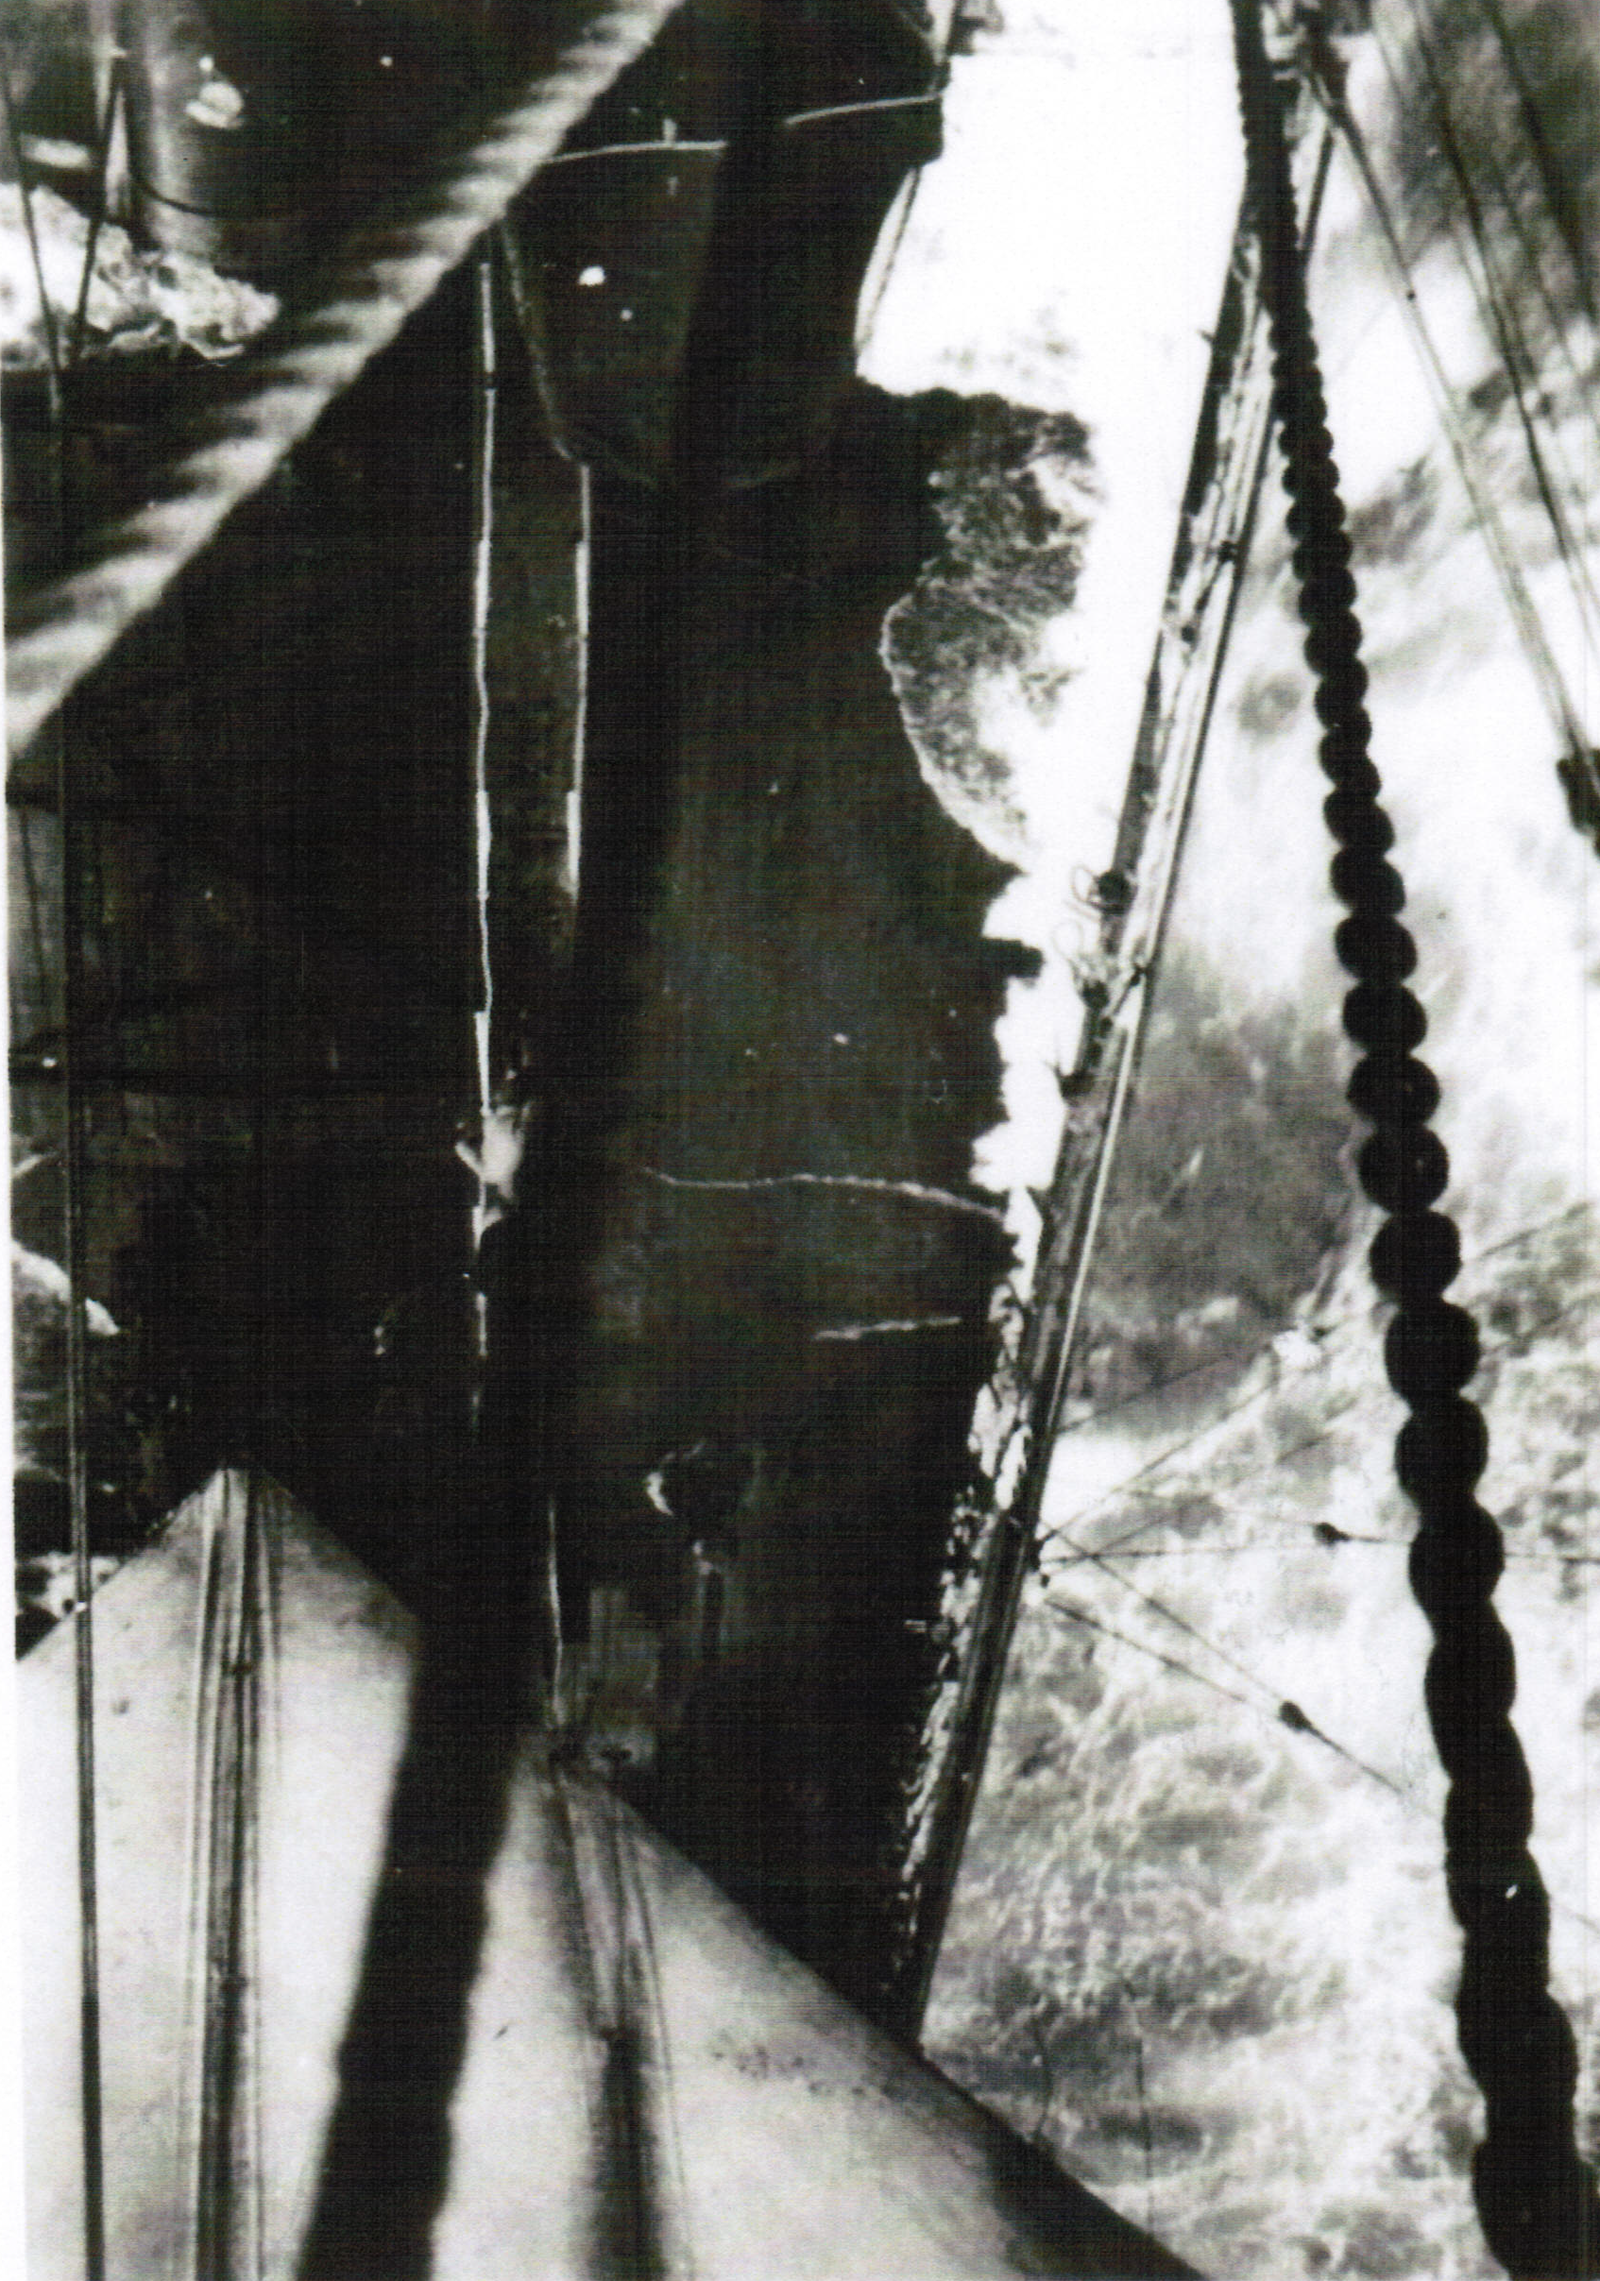
\includegraphics{./images/image012.png}
\caption{Looking down from Main Yard}
\end{figure}

\hypertarget{wednesday-17-may}{%
\section{Wednesday 17 May:}\label{wednesday-17-may}}

Wind dropped to almost flat calm -- ominous.

We spend day bending on new sails and repairing damage done by the gale.
Washing a thing of the past -- the crew are bleary eyed, dirty and
bearded. The strain of the last 10 days is showing itself on their
faces. Its every man for himself now. We are close hauled on the
Starboard tack. Sailing close hauled is very difficult to gauge, and in
any case it veers 2 points with monotonous regularity. My small boat
training is proving invaluable. Tonight we gather in fo'castle with
Coventry playing old songs on the mouthorgan. He starts to play ``Home
Sweet Home'' but is promptly stopped -- it played hell with us all. The
less one dreams on these dammed Hookers, the better!

\hypertarget{thursday-18-may}{%
\section{Thursday 18 May:}\label{thursday-18-may}}

Still messing about and getting no place. We wear ship twice during the
morning -- breeze swinging all the time but still ahead. We are within
80 miles of the South West Coast of S' America -- dangerously close, for
in the event of a S.W. gale we would be caught on a lee shore and the
ship is hardly capable of getting out of any such position. The rugged
barren coast of S. America has been the scene of many untold sea
tragedies.

The Second Mate seems to be heading for trouble.

At change of watch we were just going on deck after 2 bells when he
ordered Mensabe, a member of the other watch, to overhaul buntlines --
aloft. Mensabe replied that he was now free and was going below,
whereupon the second mate leapt at him and knocked him down.

Mensabe jumped to his feet and promptly knocked the mate down. Drawing
his knife like a flash the mate advanced on Mensabe but at this juncture
Norm Hanlon came on the scene. The mate then pocketed his knife and
asked Mensabe whether he was aware of the penalty for striking an
officer. He was invited to go to hell! With Hanlon on the scene, the
mate had not a chance as he would or could have been punished for
drawing his knife and furthermore could lose his `ticket'. The mate is
amazing chap.~Rather quiet unless roused, fine looking with a flawless
complexion - does not drink or smoke but he is a typical Mongol and is
cordially detested by the crew.

\begin{figure}
\centering
\includegraphics{./images/image013.jpg}
\caption{``Fine weather in the West Winds'' (Eight knots) (Note
triangular Cross Jack)}
\end{figure}

\hypertarget{friday-195}{%
\section{Friday 19/5:}\label{friday-195}}

The whole of the Port watch are put to scrubbing teak this morning --
cruel work in such cold weather. The crew must dip cloths in strong
caustic soda sand and chalk and finally wash with the icy salt water.

Everybody's hands are already raw and blistered and the caustic soda
causes much pain -- then to have to plunge them continually in sea water
a few degrees above freezing point -- they curse horribly.

We of the Starboard watch jeer and criticize their efforts enunciating
at great length the far superior quality of workmanship on the starboard
side of the Poop deck. They grin and bear it with frequent curses.

Our turn will come tomorrow morning and so they tell us with relish ``It
is neffer mind -- you shall scrub tomorrow Fi Fahn!''

When at wheel tonight the wind swung suddenly 3 points and as we were By
the Wind, the ship nearly caught a tack, but I had kept sufficient
steerage way so was able to steady her again on course. We are going
almost due South. Broke stem of pipe today -- ``Satan!'' However made
repairs promptly and soon back to ``old reliable''. Verily a pipe is a
great friend when at sea; tobacco seems an absolute necessity to sailors
-- they smoke incessantly. When ``risen oop'' from their bunk they
invariably reach for and light a cigarette before getting out. We have a
new moon tonight and the ``salts'' prophecy a strong wind -- from
somewhere!

At present the sea is fairly calm -- strangely so in fact -- the horizon
no longer has the appearance of the tooth edged blade of a saw but is
leveling out.

We are now almost on a level latitude with the Horn and expect that soon
we shall be squaring up and easing away to the East for the rounding.
Then with the S.W. wind on the quarter we should be around in 24 hours
and heading for those glorious warm Trade winds.

And to think that for a week when we have floundering about but 2 days
of good sailing distance away!

\hypertarget{saturday-20th-may}{%
\section{\texorpdfstring{Saturday 20\textsuperscript{th}
May:}{Saturday 20th May:}}\label{saturday-20th-may}}

Wind swung a little more West 11 am this morning and we steady on the
course South by East. We will be around Cape Horn in 24 hrs if the
existing wind holds -- if!

Just waiting for order to square up. We discuss the passing of stage one
almost incessantly. The weather really remarkable; sun has been out for
a third of the day. A heavy bank of clouds passes over and a thin
drizzle accompanies it -- then out comes the sun again in the clear
frosty air.

Two whistles? Yes. The Port watch turn out and we listen for the orders.
``Square oop'' and we are running to the Horn. The watch brace happily
-- singing and chanting. The wind freshens during the night to a brisk
Westerly.

\hypertarget{rounding-cape-horn}{%
\chapter{Rounding Cape Horn}\label{rounding-cape-horn}}

\hypertarget{sunday-21st-may}{%
\section{\texorpdfstring{Sunday 21\textsuperscript{st}
May:}{Sunday 21st May:}}\label{sunday-21st-may}}

The wind freshened very hard, the sea coming up quickly. We are squared
up and going due East -- expect to pass the Cape about midnight tonight.
Wind still harder during afternoon when Port watch bracing at 4 pm this
afternoon, Coventry and 3 others suffered a thorough wetting. Coventry
came in cursing and moaning and was just ½ way thro' changing into dry
clothes when again 2 whistles go and he is called out once more. He
clambered back into the wet clothes amid a fresh volley of curses and
out he went.

We all shriek with laughter -- it's always a joke to the other chap! Our
coldest day for the trip today -- snow and hail regularly and when these
hailstones hit you -- they hit you!

Wind goes more Southerly -- we make ten knots. As we have only 15 miles
allowed to South of Diego Ramirez, we should pass very close tonight,
allowing the natural drift to leeward.

We all cheer! At midnight -- just before -- we pass Cape Horn doing 12
knots amid snow and rain squalls but the skipper is driving the ship
along beautifully. At 2 am we square up a little and head more North to
pass the Falkland Islands, where, according to tradition, we will go
thro' the customary tortures and rites as approved by Father Neptune.

Three days of this wind and warmer weather is promised by the old hands.

Are we happy!

47 days out from the Roads in Spencer Gulf.

\hypertarget{cape-horn-to-cornwall}{%
\chapter{Cape Horn to Cornwall}\label{cape-horn-to-cornwall}}

\hypertarget{monday-22-may}{%
\section{Monday 22 May:}\label{monday-22-may}}

Bowling along merrily at 10 knots going N.E. Snowing heavily this
morning and we bend our new Upper T'Gallant sail, which blew out in a
squall during the night. Terribly cold aloft -- snow and ice in the
rigging and hands seem useless but all things are possible to God and
Sailors and up she goes.

12 noon. Big swell following almost makes the old Hooker plane along --
visibility quite fair now -- hail and snow let up.

1.30 pm. We sight land 45 miles away on the Port beam. Staten Island, a
rugged barren uninviting coast. The whole crew turn out and everyone in
state of excitement. Our course will take us past the Falklands on the
East side.

We set the main upper T'Gallant and the Spanker and the ship responds
with an added knot.

She is dipping first weather, then lee bulwarks under as she rolls with
the seas, and shoots like an arrow in the next trough.

Today no work done -- we ``Stand By''.

Tonight at 11 pm when I was at Police, sent up to unfurl Main Royal. I
lay aloft and work from lee to weather side of the yard. It was my worst
experience aloft. As soon as I had freed the lee side, the sail began to
shake and flap furiously. Repeatedly my foothold on the rope was lost
and I was left suspended by my left hand frozen on the Jackstay until my
feet had found the shaking footrope again. The yard itself was jerking
thro' the truss on the Parrel 6" each way with terrific force, besides
the bucking and shaking caused by the antics of the sail and there I was
trying to unfasten some damn stupid complicated knots some farmer had
made fast the sail with -- probably a man of the Port watch! I looked
for something to grab hold of in case I lost my grip but being right at
the peak of the mast, there was absolutely nothing.

I shouted, cursed and screamed with rage and pain and threw all caution
to the winds and went at it furiously -- using both hands on the knots.
After what seemed an eternity, probably but 4-5 minutes -- I finished --
shouted to 2\textsuperscript{nd} mate ``all clear'' and waited to
overhaul the buntlines. This done, I descended to the deck to start
bracing. I felt somehow I had achieved something and for an
unexplainable reason was in extraordinary good humour for the rest of
the watch.

\hypertarget{tuesday-23rd-may}{%
\section{\texorpdfstring{Tuesday 23\textsuperscript{rd}
May:}{Tuesday 23rd May:}}\label{tuesday-23rd-may}}

Ship going splendidly with following sea and wind.

We sighted land again today away to Port and 25 miles distant. On our
course we expect to pass within 7-8 miles from the coast. Beauchise
Island -- a French possession just off the South East Coast of the
Falklands.

Tonight when at Police two bells rung and I dash out to see the
2\textsuperscript{nd} mate rushing for'ard along the Flying Bridge.

2 Bells -- a light sighted to Port. There it is -- very dim - the
Lighthouse on the N.E. coast of Falkland Islands (North Island).

We watch the light grow brighter as we draw level, but can see no land
in the darkness.

The Skipper has been lucky with his landfall and consequently has been
able to check his Chronometer. The weather is becoming decidedly warmer
day by day and our progress is most satisfactory.

Suffering with bad feet. The continual wetness of socks has caused skin
to go soft and is peeling off in great blisters, leaving a horrible mess
to walk on.

\hypertarget{wednesday-24th-may}{%
\section{\texorpdfstring{Wednesday 24\textsuperscript{th}
May:}{Wednesday 24th May:}}\label{wednesday-24th-may}}

Scrubbed teak most of the day. Ship doing steady 10 knots going N.E. and
we cross 50° South.

Bend on new big Cro'jack to replace the small tri angular one used in
the West winds. The smaller tri angular sail has a big advantage over a
square sail, in that it can be furled much more quickly and easily in a
crisis.

Carrying every stitch of canvas

\begin{figure}
\centering
\includegraphics{./images/image014.png}
\caption{Solid water coming over. (I was taken about 30 ft along the
deck by this one)}
\end{figure}

\begin{figure}
\centering
\includegraphics{./images/cape-horn.png}
\caption{Cape Horn and Islands surrounding etc at Southern peninsula
South America}
\end{figure}

\hypertarget{thursday-25-may}{%
\section{Thursday 25 May:}\label{thursday-25-may}}

No change in weather.

The cook is seeking a new pair of trousers and is offering wonderful
opportunities to obtain supplies of condensed milk and other luxuries to
obtain a pair but the ones we hastily offer him are not suitable.

Confound the luck!

Feet still bothering me -- sore as hell!

The wind lightened at 3 am on

\hypertarget{friday-265}{%
\section{Friday 26/5:}\label{friday-265}}

The weather becomes more favourable -- sun appears. When at wheel this
morning saw a whale about 50 yards from the ship to leeward -- spouting
and causing a disturbance in the water. This is the third whale I have
seen on the trip but I think I failed to record on the two other
occasions. When aloft last week was rebuked for taking risks in furling
sail by the ``Old Man''.

We took in all staysails and I was told aloft to make fast Jigger
T'Gallant Staysail.

When the sail was lowered the wind was fresh from abeam and the sail
wrapped itself around to lee of several of the braces and the Lower
T'Gallant halyard.

This prevented the sail from being properly hauled in and I was expected
to do the rest.

I tried for some minutes without success and was fast becoming ``hot
about the collar'' and decided to climb around the sail itself and
pummel it with my feet.

I quickly worked around to lee hanging on to upper canvas and kicking
the sail below -- a maneuver which was proving eminently successful when
I heard two frantic voices shrieking from the Poop.

Glancing down I saw the 2\textsuperscript{nd} mate and the ``old man''
gesticulating wildly and shouting a lot of unintelligible orders and
advice and gathered I was to return to the safety of the footrope. This
I did and another man was sent aloft to assist in finishing the job.
Upon reaching the deck the Captain called me up --

``Saaten -- You shall be careful -- you shall be careful for your life
for Helvita (For Hell's sake) Alright'' and dismissed me.

The second mate also received a wigging for sending only one man to do
this particular job.

This sail is the worst to furl on the ship -- invariably trouble is
experienced when the wind abeam. However \ldots!

Everybody happy -- the weather is great -- passed 45° South today.
(Lat.)

Being 40 odd days since my hair has been combed and about 2 months since
last shave I am, with all the others, going to clean up tomorrow.
Shaving and haircutting is the topic of the ship at present.

\hypertarget{saturday-275}{%
\section{Saturday 27/5:}\label{saturday-275}}

Good weather still prevailing but sure enough I was caught in clean
clothes and told to heave and carry coal. We were 3 hrs at it and with
the mate watching the whole time, had no chance of a let up. We smoked
down in the forepeak the whole time -- Phillips and I did the shoveling
-- a black, wet, burnt out cigarette butt drooping from your lips makes
all the difference.

Washed our fo'castle out today -- thus working hard for 10 hours without
a break except for ``meals'' -- ``Pigs blood Pancakes'' again.

We brace twice following -- the 2\textsuperscript{nd} mates fault.

After a very tiring day we come to

\hypertarget{sunday-285}{%
\section{Sunday 28/5:}\label{sunday-285}}

With the weather a little cooler and cloudy but any conditions seem
pleasant these days.

Wind light S.W. -- 4-5 knots.

Traded 100 cigarettes for ¼ lb tobacco with the cook.

Everyone has bath and shaves today.

Bos'un, carpenter and Donkeyman spent all the morning cutting hair.

Remarkable to see the difference in the crew -- they all look a dirty
hard boiled lot of bums, but a bath shave and haircut rehabilitated them
to the status of human beings. I could scarcely recognize ``Mac'' -- he
looks but a boy of 18 -- Coventry much the same; whereas with a beard
they might be anything from 20 yrs to 35 yrs.

Wind freshened ahead tonight and we do 11 ½ knots `by the wind' -- full
sail.

\hypertarget{monday-29-may}{%
\section{Monday 29 May:}\label{monday-29-may}}

Risen up at midnight to come on deck and found it raining heavily but
free night and n whistles I turn in again.

At 8 am we come on deck once more to find conditions fairly rough, the
wind is howling like a thousand devils and the sea white with foam. The
Port watch have evidently furled the Royals during the night.

We take in upper T'Gallants in rainsquall and I was soaked again, but
there is a very pleasant difference in the temperature these days making
work aloft much more enjoyable. Rutherford ``went on the wheel'' on
Friday night last. It has taken him since then to swallow his pride and
tell us of his experience. He started taking wheel only last Wednesday
with Coventry and on Friday went over it -- pretty fast work!

Going over the wheel is a nasty and sometimes dangerous experience and
the helmsman is lucky if he escapes with only a few bruises.

Rutherford was lucky!

He evidently had a slack grip on the spokes of the wheel when a sea
kicked the rudder, spinning the wheel. He quickly grasped the spokes to
stop the spinning but went like a flashover the top and was hurled
against the steel roof and wall.

We jeer at him!

Coventry rang two bells in error last night when at Lookout and the
Hands turned out thinking a ship had been sighted. He was duly cursed.

\begin{figure}
\centering
\includegraphics{./images/image015.png}
\caption{``Beauchise Island'' (just past Cape Horn)}
\end{figure}

\begin{figure}
\centering
\includegraphics{./images/image016.png}
\caption{``Mac'' -- myself -- Coventry. All dressed upon a Sunday after
our first shave for nearly two months}
\end{figure}

\hypertarget{tuesday-305}{%
\section{Tuesday 30/5:}\label{tuesday-305}}

Breeze dropped away to a flat calm during the night and leaves us
rolling heavily in the oily swell which however is rapidly going down.
Rather miserable day -- rain all morning but mixed blessing, as this
enabled us to replenish washing water supply which has been exhausted
for some time. After we had all shaved on Sunday and since then all eyes
were turned critically on one another to see what we really looked like.
I was agreeably surprised to see how all our complexions had improved.
Whether this was due to the extreme cold weather or freedom from shaving
I don't know, perhaps a little of each but we all now possess clear pink
faces with the real apple cheeks.

Another thing now apparent -- the growth of ones beard is astonishingly
slow.

\hypertarget{wednesday-31st-may}{%
\section{\texorpdfstring{Wednesday 31\textsuperscript{st}
May:}{Wednesday 31st May:}}\label{wednesday-31st-may}}

We scrubbed white paint all day and gradually the ship is becoming a
thing of beauty. At night, when the moon comes out shining on the
freshly washed whiteness everywhere, the great old with the crowding
sails looks very romantic and attractive, specially when the sea is bit
up with a full moon.

We have been practically becalmed all day with the sun out most of the
time, very pleasant conditions prevail generally.

With the coming of the warmer weather the crew lounge and wander about
the decks at night, and social life improves wonderfully -- everyone
friendly and showing good fellowship.

Tonight when bracing I was suddenly sick and spent the next 12 hours in
my bunk feeling deadly, until on

\hypertarget{thursday-1-june}{%
\section{Thursday 1 June:}\label{thursday-1-june}}

About 9 am the passenger -- medical student -- came down and diagnosed
the trouble as due to sudden change from cold to warm weather -- quite
frequent on ships so he informed me.

Anyway, with some medicine and sleep I soon recovered.

My recovery so quickly rather disappointed the 1\textsuperscript{st}
mate -- that great tall stringbean of a sailor. He's a great chap and
inquired twice after me -- each time bringing with him a large bottle of
Castor oil. This is his remedy for all ills and he hovered about me
until I went on deck at midday.

With no wind, we clew up the courses and on the Jigger mast alterations
and repairs are being effected -- stays and shrouds and braces are being
moved as the mast has been found to be badly cracked and weakened about
80 ft from deck. As the Captain anticipated a blow, this work is being
rushed.

Verily the rigging on this ship has a day to day existence -- its rotten
from truck to keep and absolutely unsafe to work aloft. Even our chain
sheets are breaking and worn out. We can't take in sail without
buntlines breaking. Hands packing up with the continual use of Caustic
Soda.

\begin{figure}
\centering
\includegraphics{./images/illustration.jpg}
\caption{Very rough sketch - sails etc.}
\end{figure}

\hypertarget{friday-2nd-june}{%
\section{\texorpdfstring{Friday 2\textsuperscript{nd}
June:}{Friday 2nd June:}}\label{friday-2nd-june}}

Our expected blow arrived -- from the North with a little West in it.

Midnight: 3 whistles. All Hands.

Sail comes in rapidly : Royals, Upper and Lower T'Gallants, mainsail and
Cro'Jack and T'Gallant Staysails all come in. Although it's blowing like
hell, working aloft is a joy -- marvelously bracing and exhilarating and
no frozen fingers or icy rain to impede your work.

We laugh joyously as we fight the great Sails up there 160ft aloft. The
satisfaction of pitting yourself against a seemingly impossible task,
the joy of physical perfection and the risks involved make a sailors
life a happy one.

We go below singing and smoke and sleep. Three whistles? Yes. We go out
again to find the ship plunging madly into the terrific seas -- the wind
has risen to cyclonic force and is whipping the tops of the waves -- the
sea is a blurred white mass heaving and descending dangerously. No
Lookout is kept -- she is dipping her fo'castle head right under the
seas which comes crashing over and sweeping along the decks and anyone
on the fo'castle head would be in danger of being swept overboard.
Before Lookout was abandoned, the chaps had lashed themselves to the
pin-rail.

We learn later that it is the edge of a South Atlantic cyclone. The Fore
staysail comes in -- the Port watch begin to return to their fo'castle
-- their watch below. But they were not yet to enjoy the comforts of the
Free watch below. With a terrific report a shackle breaks on the fore
Lower Topsail weather sheet and the Sail begins to shake in all
directions. Three whistles again. The Port watch return for'ard and all
Hands jump aloft and take in the sail. The wind pinned me to the
ratlines and my clothing seemed as if pulled at by a thousand unseen
Hands. This is `wind de luxe'.

The Captain estimates it at over 60 mph.

The ship heaves and pitches under practically bare poles.

\hypertarget{at-3-am-on-saturday-3rd-june}{%
\section{\texorpdfstring{At 3 am on Saturday 3\textsuperscript{rd}
June:}{At 3 am on Saturday 3rd June:}}\label{at-3-am-on-saturday-3rd-june}}

It began raining in torrents and I expected the wind fell away. We catch
rainwater.

By 4 am the wind had dropped to a mild S.W. breeze and we commence
setting sail again. By 8 am practically all sail set -- the Jigger mast
left bare as not safe.

Making 4-5 knots again the left over swell of gale, which however,
should soon be knocked back now as the wind has veered. Once more
everyone saying the S.W. wind will swing to S.E. and we will get the
warm S.E. trades. I wonder!

This has been prophesied so often now that until they arrive I'm not
worrying but in spite of trying not to anticipate, if as good as tales
told, they will certainly be Heavenly.

What the hell does it matter anyway? Smoking again after 2-3 days
abstinence -- sure sign of recovery from sickness a few days ago. Breeze
left us midday and we lie becalmed. Spend watch chipping rust.

\hypertarget{sunday-4-june}{%
\section{Sunday 4 June:}\label{sunday-4-june}}

Dawns a promising day but with a mere drift of air -- until 10 am when
wind freshens and we sail by the wind about 1 point west of North with
an ominously black horizon to windward. Captain not happy about the
weather so in come the Royals. I took Main Royal single handed -- first
time. Getting pally with the cook -- he's a nitwit but, well -- tact and
diplomacy and all that sort of thing !!

Last year he tells us he was ordered aloft (he was then ordinary Seaman)
to take in Fore Royal.

He refused, stating that the rigging was not safe and got away with it.
After the recent blow, our rigging is looser than ever.

What a ship! Everybody predicts this voyage to be her last unless she is
re-rigged. However, the Captain is showing rare good judgment and is
nursing her along very well -- that's obvious.

Cookie made us apprentices a ``cake'' `under the lap' today -- this
`crawling' racket has its advantages. He also lets us have 3 tins of
condensed milk weekly -- for which we give him cigarettes and clothing.
It is fast developing into a National backscratching Competition.

\begin{figure}
\centering
\includegraphics{./images/image017.png}
\caption{The Cook (with the hat on)}
\end{figure}

As soon as we come on deck at 7 pm tonight we take in Upper T'Gallant
amid rain and a hard driving wind which however strikes moderately warm.
The Port watch tack ship as the wind later veered to N.W. by W -- having
gone right around the Compass in the last 3 days.

Further signs of a cracking up ship were found yesterday -- two or three
plates for'ard -- fortunately above waterline have been pounded open and
the Jib-boom has been the subject of a close scrutiny -- the rivets have
been torn off at the base and apparently it weaves around when she dips
heavily.

Ah well! She may get us to England!

Haula came down from the wheel tonight and informed us that if we
continue with the present wind we will call at the Island of Trinidad
where skipper wants to shoot some game. Thus far he has been
concentrating on the poor inoffensive albatross -- with indifferent
results happily. Started third period of ``Percy'' -- back to the slimy
greasy dishwashing and filth for a week.

``Who will sell their farm and come to sea?''

But I am enjoying the life. The good is bad, the work harder but now I'm
used and toughened to it, find everything quite enjoyable. There are
times of course \ldots\ldots!!

\hypertarget{monday-5th-june}{%
\section{\texorpdfstring{Monday 5\textsuperscript{th}
June:}{Monday 5th June:}}\label{monday-5th-june}}

Light drizzling rain all the morning -- we catch rain water and chip
rust in the rigging. Upper T'Gallants still furled although we have been
practically becalmed all day (since daylight).

This afternoon rather late, the weather cleared over more or less but
left great banks of grotesque looking clouds which made a spectacular
sunset.

``A Sunset at night -- the Sailor's delight.''

We all wonder!

`Glass' still fairly low and we continue to flounder in the doldrums.

We are now right between two recognized wind zones; the Westerlies which
we have just left and the S.E. Trade winds for which we wait. Tonight an
absolute flat sea with mild air and a lazy swell which makes a perfect
night at sea -- the best experienced on the trip thus far.

It was in similar conditions last year on this ship that the vessel was
struck by a gale or squall of wind known as the Pamperos.

This wind originates in the Pampas Mountains and is very destructive to
shipping near the coast and is felt for many leagues at sea. As the wind
(usually from S.W.) can develop a velocity of 90 mph, somewhere about
force 12, it will be understood what a menace it is. However the ship
weathered the storm at the cost of a few blown sails on this occasion.
We set Upper T'Gallant and Royals tonight -- I had a hard job loosing
the fore Royal, as with continual rain of the past 36 hrs, the gaskets
(rope lashings) around the sail had shrunk and the knots tightened to a
very high tension.

A perfect night and on

\hypertarget{tuesday-6-june}{%
\section{Tuesday 6 June:}\label{tuesday-6-june}}

as perfect a dawn.

We chip rust on Turnbuckles in sunshine and light West by N. wind.

By 11 am however clouds had appeared thick up to weather at 2 pm blowing
hard and raining -- Royals and T'Galants furled.

The wind swings farther ahead and we brace accordingly ``By the wind''.
Wind changes several times more during the night and again we brace in a
brisk breeze which

\begin{figure}
\centering
\includegraphics{./images/illustration2.jpg}
\caption{The action of bracing: - the yards on swing by brace winches to
suit the direction of the wind. Sails as shown drawn with continuous
line, the wind would be}
\end{figure}

\hypertarget{by-wednesday-7th-june}{%
\section{\texorpdfstring{By Wednesday 7\textsuperscript{th}
June:}{By Wednesday 7th June:}}\label{by-wednesday-7th-june}}

Had dropped to a gentle steady S'Wester and up go the T'Gallants and
Royals and we move steadily Northwards.

I am being used a lot for work aloft and liking it -- in brilliant
sunshine the work up there is a great improvement and I do not hurry
down to deck to ``Knacker Roost'':- (chip rust).

\begin{figure}
\centering
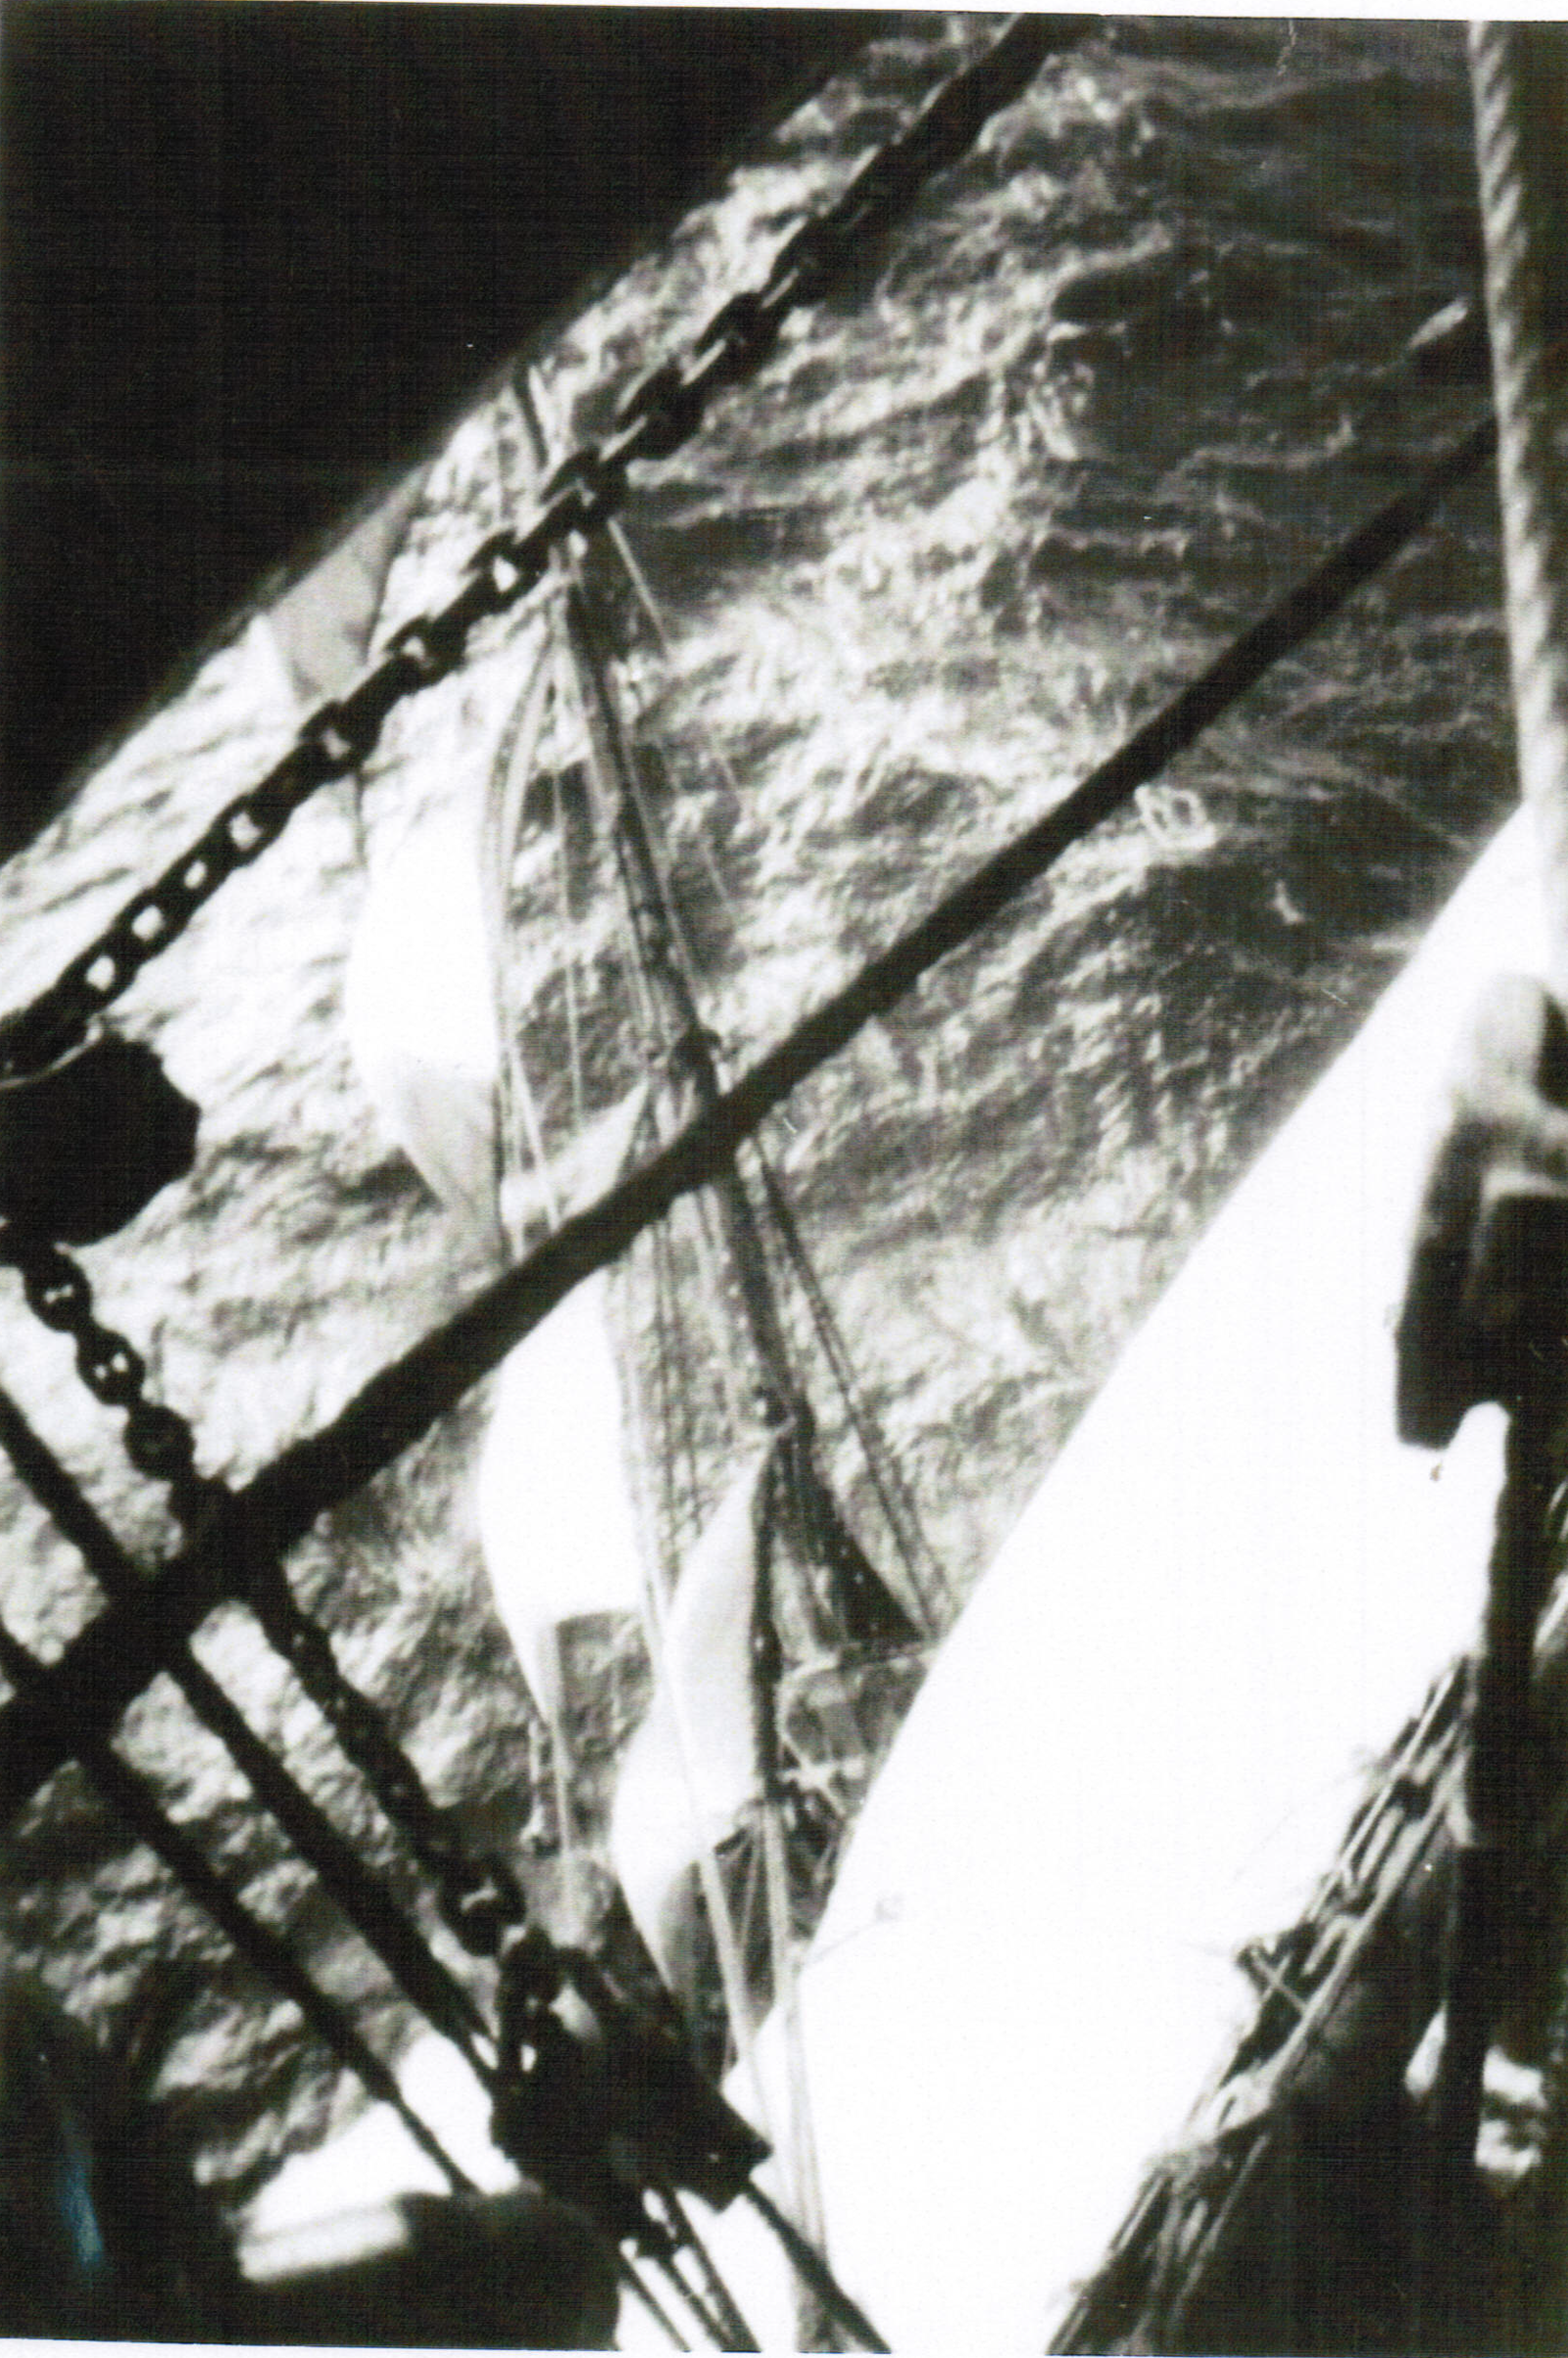
\includegraphics{./images/image018.png}
\caption{Aloft in sunshine (Note our 60ft Jib-boom)}
\end{figure}

\hypertarget{thursday-8th-june}{%
\section{\texorpdfstring{Thursday 8\textsuperscript{th}
June:}{Thursday 8th June:}}\label{thursday-8th-june}}

We chip rust. Are now on the steamer route from Rio de Janeiro to Cape
Town and hoping to sight one and hear some news. Is Hitler dead? No,
that's too much to expect! Are we at war? Or is everything the same as
ever?

Little we care or worry -- isolated as we are nothing seems to matter.
But it's a grand life!

The 1\textsuperscript{st} mate, Johannson, Donkeyman are Idlers (Daymen)
from today. This means that they work normal working hours 7 am to 5 pm
and have the nights entirely free. The watches are thus reduced to six
men a watch.

\hypertarget{friday-9th-june}{%
\section{\texorpdfstring{Friday 9\textsuperscript{th}
June:}{Friday 9th June:}}\label{friday-9th-june}}

Clear sunny weather -- light W by N breeze. We chip more rust. Crew
working in shorts and shirt -- quite sufficient clothing in the pleasant
conditions prevailing.

Cigarette paper stocks have risen to unbelievable heights. The crew are
desperately short of Papers and high prices are being offered for every
one packet. The shortage of papers gave rise to an amusing incident.

Rutherford telling the passenger how short we all were asked him if he
was able to spare any. Shaking his head dubiously the passenger offered
to find out, with the remark ``I'll check my calculations (that's rich)
and see!'' After spending 5 minutes below he came up:- ``I have checked
my calculations and find that I can spare six''.

Rutherford, thinking what 6 packets meant to us, thanked him
enthusiastically and took the tine containing the six packets and came
into the fo'castle to share them out. Opening the tin he found six --
yes you have guessed it! -- SIX papers! That would last us about 10
minutes. Rutherford then returned the tin, thanked the Passenger gravely
and bursting with laughter came below. Haw -- guess the passenger would
not appreciate the joke!

\hypertarget{saturday-10th-june}{%
\section{\texorpdfstring{Saturday 10\textsuperscript{th}
June:}{Saturday 10th June:}}\label{saturday-10th-june}}

More glorious weather. Had 1\textsuperscript{st} haircut today on ship
and a bath -- 3 baths in 3 days. Simply had to record this!

The wind ahs swung almost due North and we are on Port tack going only a
little better than East. The wind varies frequently.

This swinging of the wind makes the helmsman's job a hard one when ``By
the Wind''. I am always trying to come up closer to the wind as it means
much over a days run but it is extremely annoying and not a little
fatiguing after much careful effort to see the Royals blown abrace and
the Upper T'Gallants aquiver.

Most of the chaps set a compass course allowing a variation of about 1
point in the wind -- this saves much trouble but does not always get the
best out of the ship.

We laze about the after Hatch on sails during the afternoon and try
feats of strength etc and yarn and smoke in the warm sunshine. Our only
clothing is shorts and sandshoes.

\hypertarget{sunday-11th-june}{%
\section{\texorpdfstring{Sunday 11\textsuperscript{th}
June:}{Sunday 11th June:}}\label{sunday-11th-june}}

When at Lookout watch 4-8am saw the most glorious sunrise I can
remember. From 5.15 am when a light glow appeared to the East until 7
am, I -- we all - watched the transformation of the sky from semi
darkness to a marvelously delicate tint of pink in the high semi circle
of streaky clouds which slowly developed to the full blood red of a
perfect dawn. No art can reproduce such colours as these.

Having had but 4 hrs sleep in the past 28, I turned in quickly at 8
bells and wake to find sky overcast and wind freshening. Sure enough
just after I get to wheel it rained as it can only rain the tropics. I
had a glorious shower for an hour and revel in it, clothed in shorts
only. We carry rain water and also replenish the ships tanks from a
great canvas water catcher.

Watch below and I turn in. I write my diary and suddenly note the ship
leaning to what was windward. I learn that the helmsman has put the ship
in Irons. The Captain, 1\textsuperscript{st} and 3\textsuperscript{rd}
mates are tearing around in circles and is Mensake popular? Much!!!

He must have fallen asleep at the wheel in the rain which is still
coming down fairly hard.

The Cook made us a huge cake today -- on return I give him a packet of
Lifebuoy soap which he has coveted for some time.

It is remarkable the interest we take in every trivial little event. I
expect this is natural after being so long at sea which no outside
interest -- we live a carefree day to day existence -- nothing matters.

By nature I am indolent so that lack of excitement and social life
worries me not in the least, although I had anticipated missing the
humdrum city life left behind. But No\ldots!

Great scott! What's going on outside? I go to the door of our fo'castle
and listen.

Things are in a hell of a mess! The ship is flat aback, the wind has
increased and is very hard and it is raining heavily.

The Skipper is really drunk and falling all over the deck. The
1\textsuperscript{st} mate is little better and the
3\textsuperscript{rd} is useless anyhow.

God, how that wind howls! The Skipper is shouting orders -- the
1\textsuperscript{st} mate promptly contradicts them and bedlam reigns.

Sails and Yards swing dangerously above, groaning and creaking under the
terrific strain.

She's caught aback alright -- will the masts hold?

It is pitch black outside and to a long story short, the crew take
charge and get her back on the course after 3 ½ hrs but she's under
shortened sail -- Royals and Upper T'Gallants tucked away. `'Mac' and I
chuckle to ourselves -- we are free watch and in our bunks and enjoying
the Port watch's' misery.

Coventry and Rutherford (Port watch) come below cursing that the
starboard watch were not called out to assist in the emergency. I told
them that if the Port watch had such ``farmers'' for helmsman they must
expect such work.

As the subject of steering is rather a sore point with them (for reasons
previously diarised) ``Mac'' and I found ourselves quickly involved in a
furious argument as to the merits of the two watches but with the usual
climax of ``Go to Hell'' from both sides. (Just one big happy family
!!!)

It rained all night and wheel turn was just another bath but ship nice
and easy to handle.

\hypertarget{monday-june-12th}{%
\section{\texorpdfstring{Monday June
12\textsuperscript{th}}{Monday June 12th}}\label{monday-june-12th}}

brings a grey wet dawn and we drag water barrels for'ard. Most
unseasonal weather. By 1.30 pm the weather had cleared a little but the
day closed with the sky still overcast.

Today we officially enter the Tropics -- passing over 23 1/2° South
latitude -- the Tropic of Capricorn and from today we are entitled to
lime juice allowance and jam is also substituted for margarine. This
applies until we cross Topic of Cancer 23 1/2° North latitude.

Spent tonight in arguments generally.

\hypertarget{tuesday-13th-june}{%
\section{\texorpdfstring{Tuesday 13\textsuperscript{th}
June:}{Tuesday 13th June:}}\label{tuesday-13th-june}}

Came Tuesday 13\textsuperscript{th} June with improved weather -- the
wind has fallen off tho' and we are full \& by on the course. Sun breaks
thro' at 2 pm and weather clears when light N.W. breeze arrives -- we
square up a little and set the Royal - I had a glorious hour aloft in
the sunshine.:

Ayliffe was enthusing about his approaching home coming and made me feel
quite homesick.

Wind continues swinging and I suspect we are at last going to feel those
belated S.E. Trade winds. We shall know within 48 hrs anyway.

\hypertarget{wednesday-14th-june}{%
\section{\texorpdfstring{Wednesday 14\textsuperscript{th}
June:}{Wednesday 14th June:}}\label{wednesday-14th-june}}

Clear sunny morning with brisk S.E. wind and we brace accordingly going
North. This wind is believed to be the beginning of the Trades and
everybody jubilant.

This is the weather -- reminds me of our glorious S.W. winds and
sunshine in South Australia.

Our watch further reduced today -- `Mac' and Haula are now Daymen.
Although the watch has been reduced, it will throw little more hard work
on us, as both `Mac' and Haula, being old hands, rarely worked aloft and
invariably got the soft jobs -- the privilege of long service.

Furthermore we do not expect to touch the braces for any period up to 21
days, something not uncommon. Just imagine it! Sailing over thousands of
miles without touching the sheets.

No wonder sailors go into rhapsodies about the S.E. and N.E. Trades
winds these warm but brisk winds which send you half way across the
world.

We now begin to change the sails -- the good sails used thus far are
taken off and replaced by older and lighter sails -- the rain and heat
quickly rots the canvas.

We changed the Foresail today.

\begin{figure}
\centering
\includegraphics{./images/image019.png}
\caption{``Changing Sails'' The new good sail has been furled and is
just going to be sent down. I am just visible on outer end yard arm
unshackling sheet.}
\end{figure}

\begin{figure}
\centering
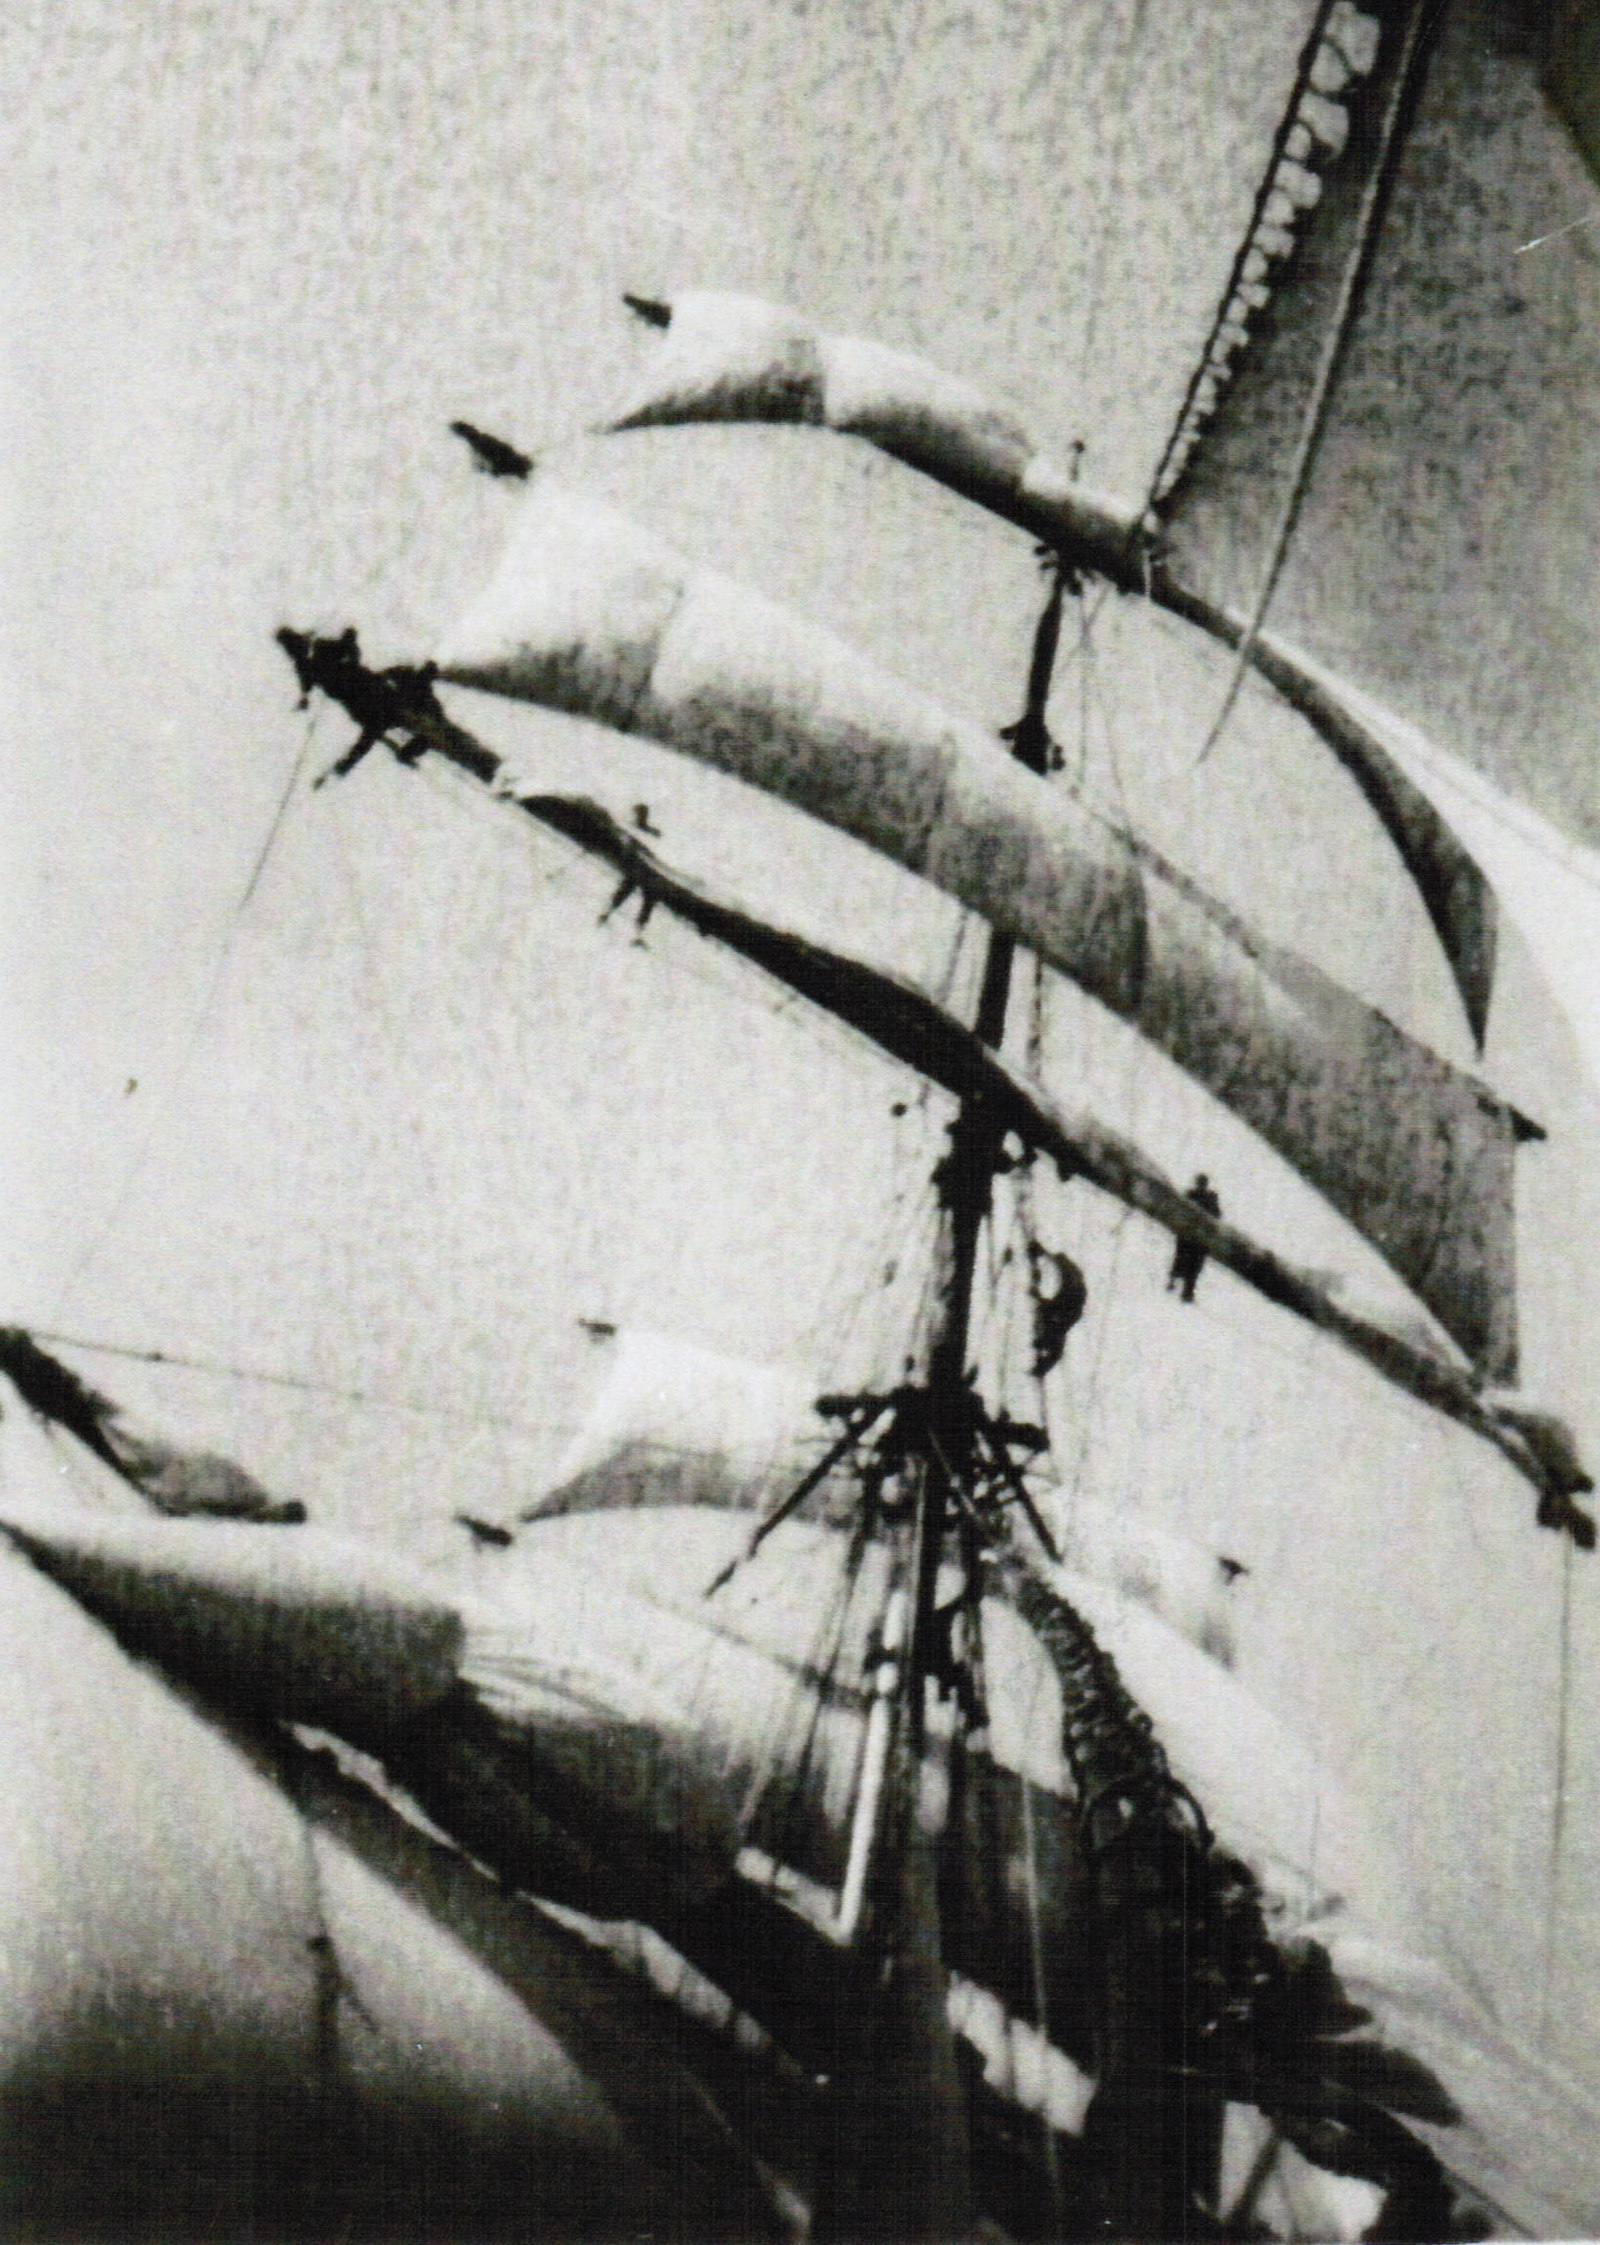
\includegraphics{./images/image020.png}
\caption{``Cutting the seizings when changing sail''}
\end{figure}

\begin{figure}
\centering
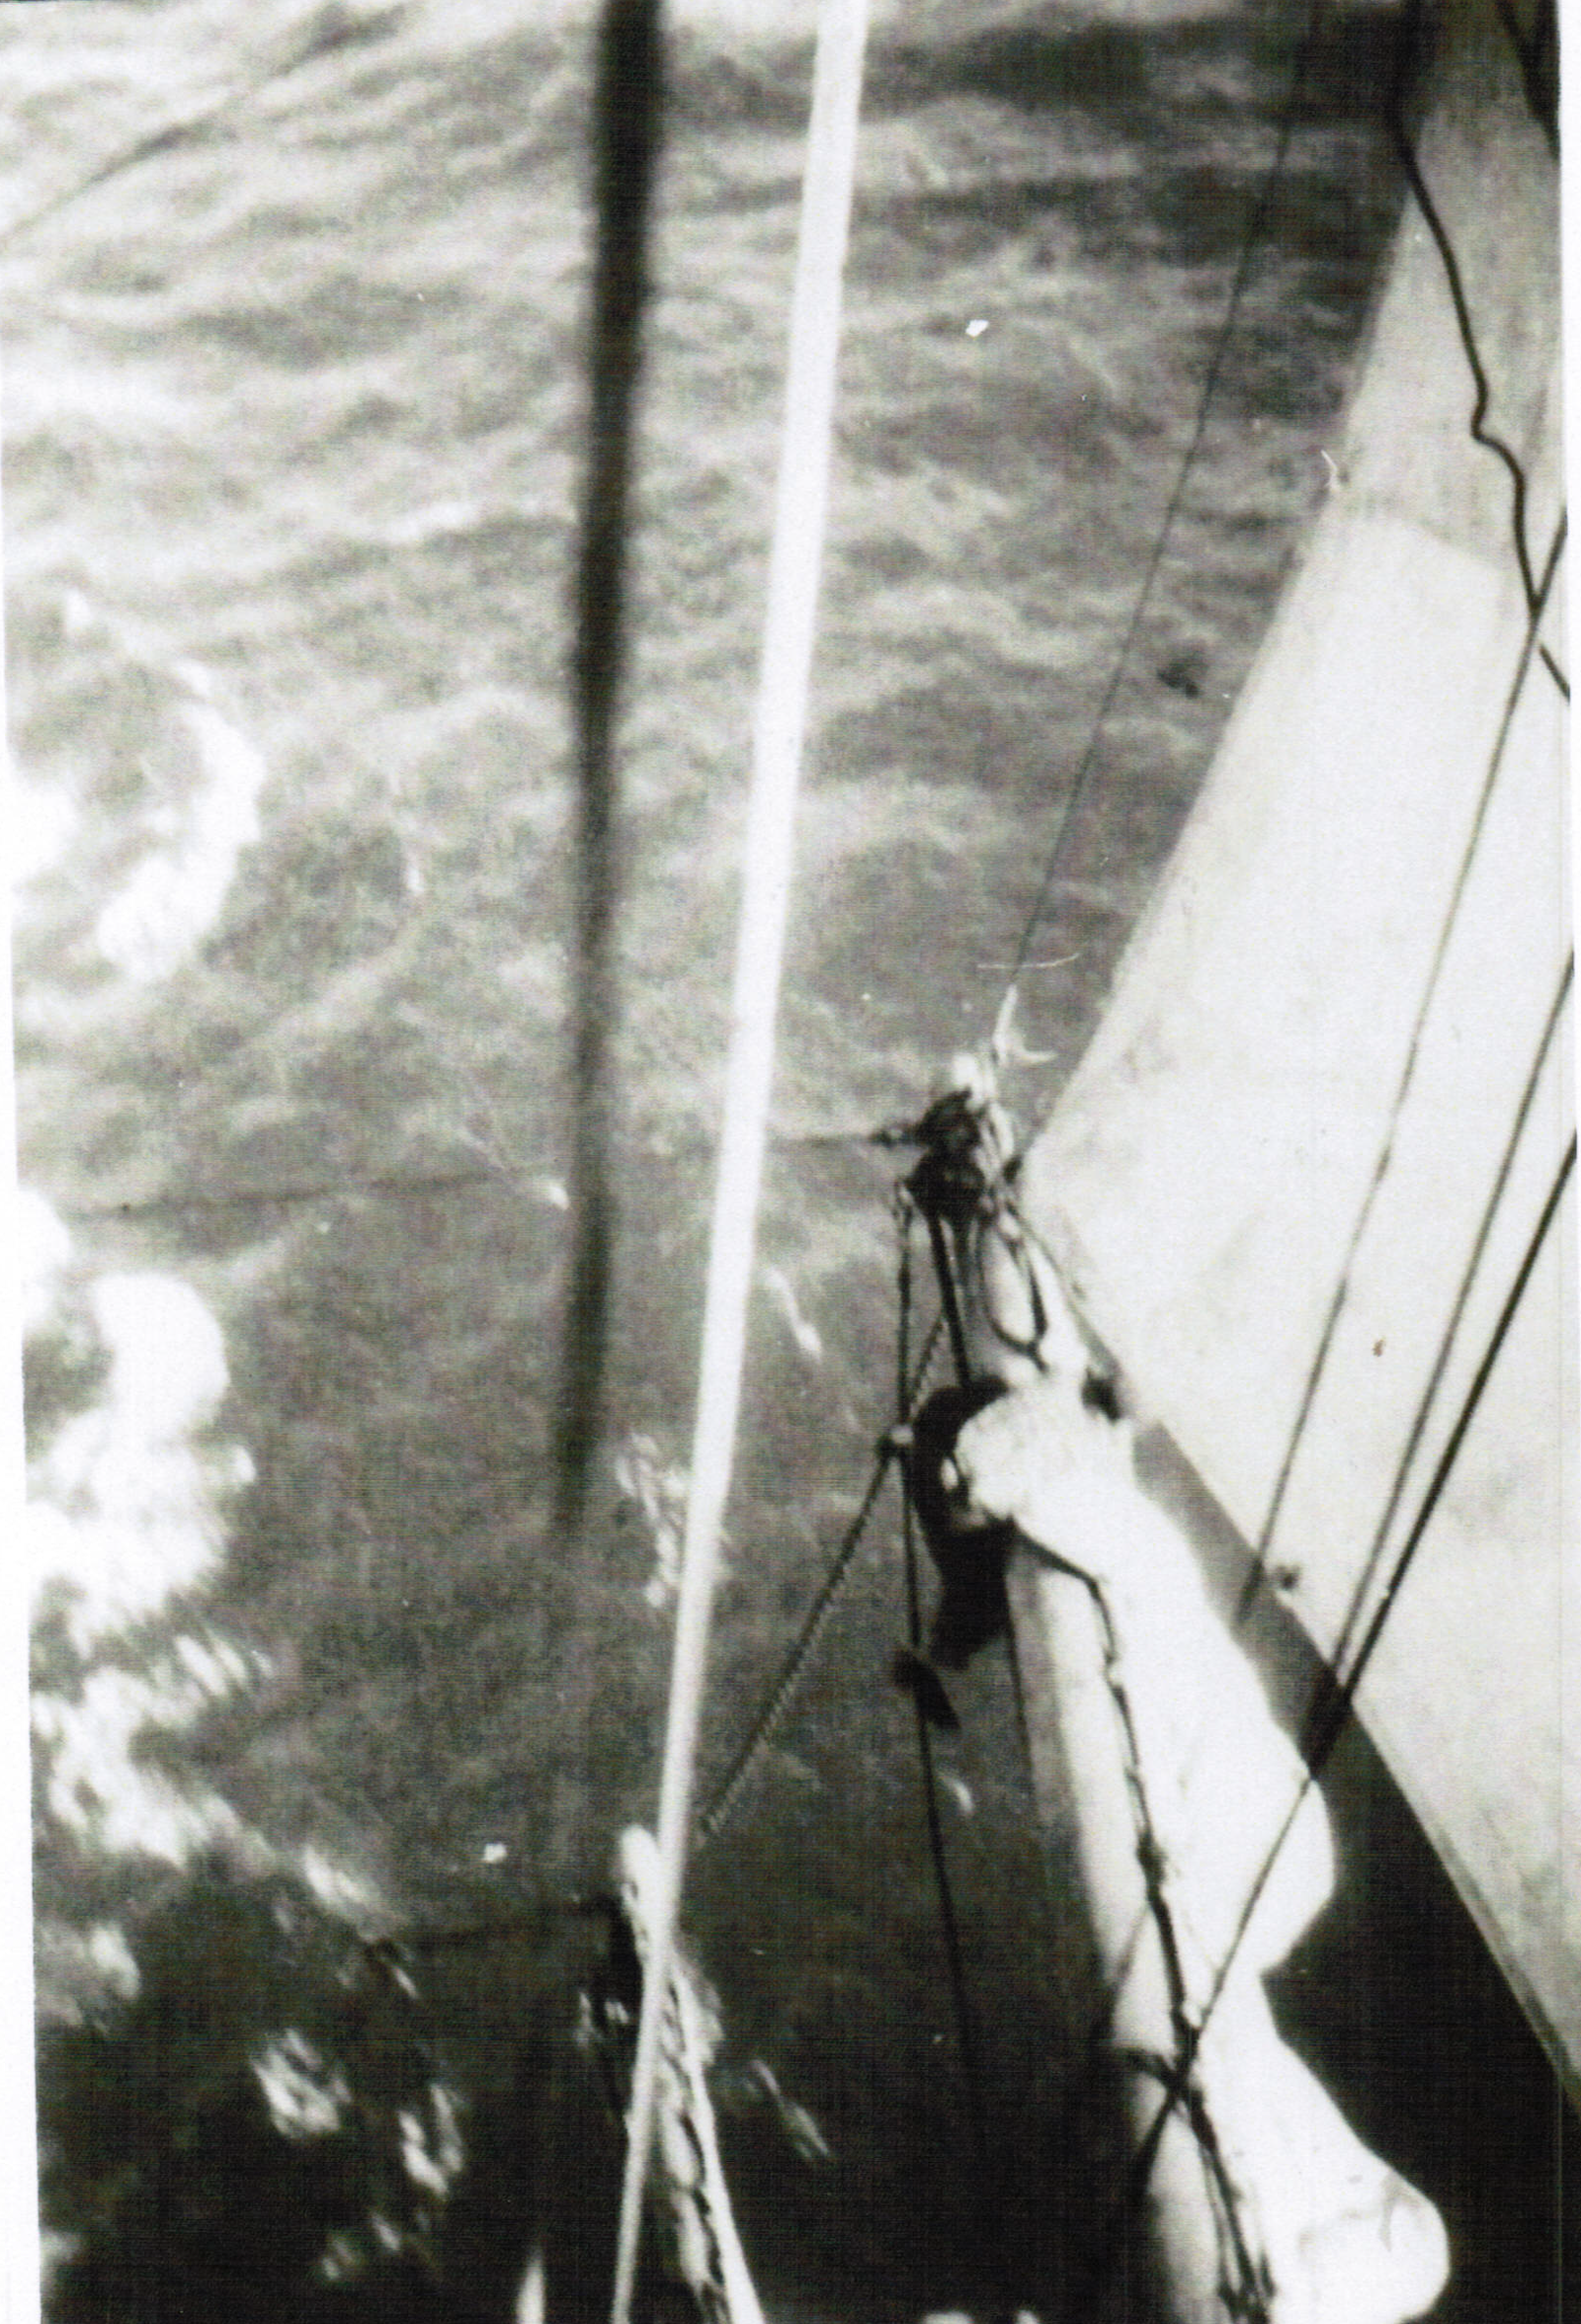
\includegraphics{./images/image021.png}
\caption{`Mac' arguing with a lower T'Gallant}
\end{figure}

\begin{figure}
\centering
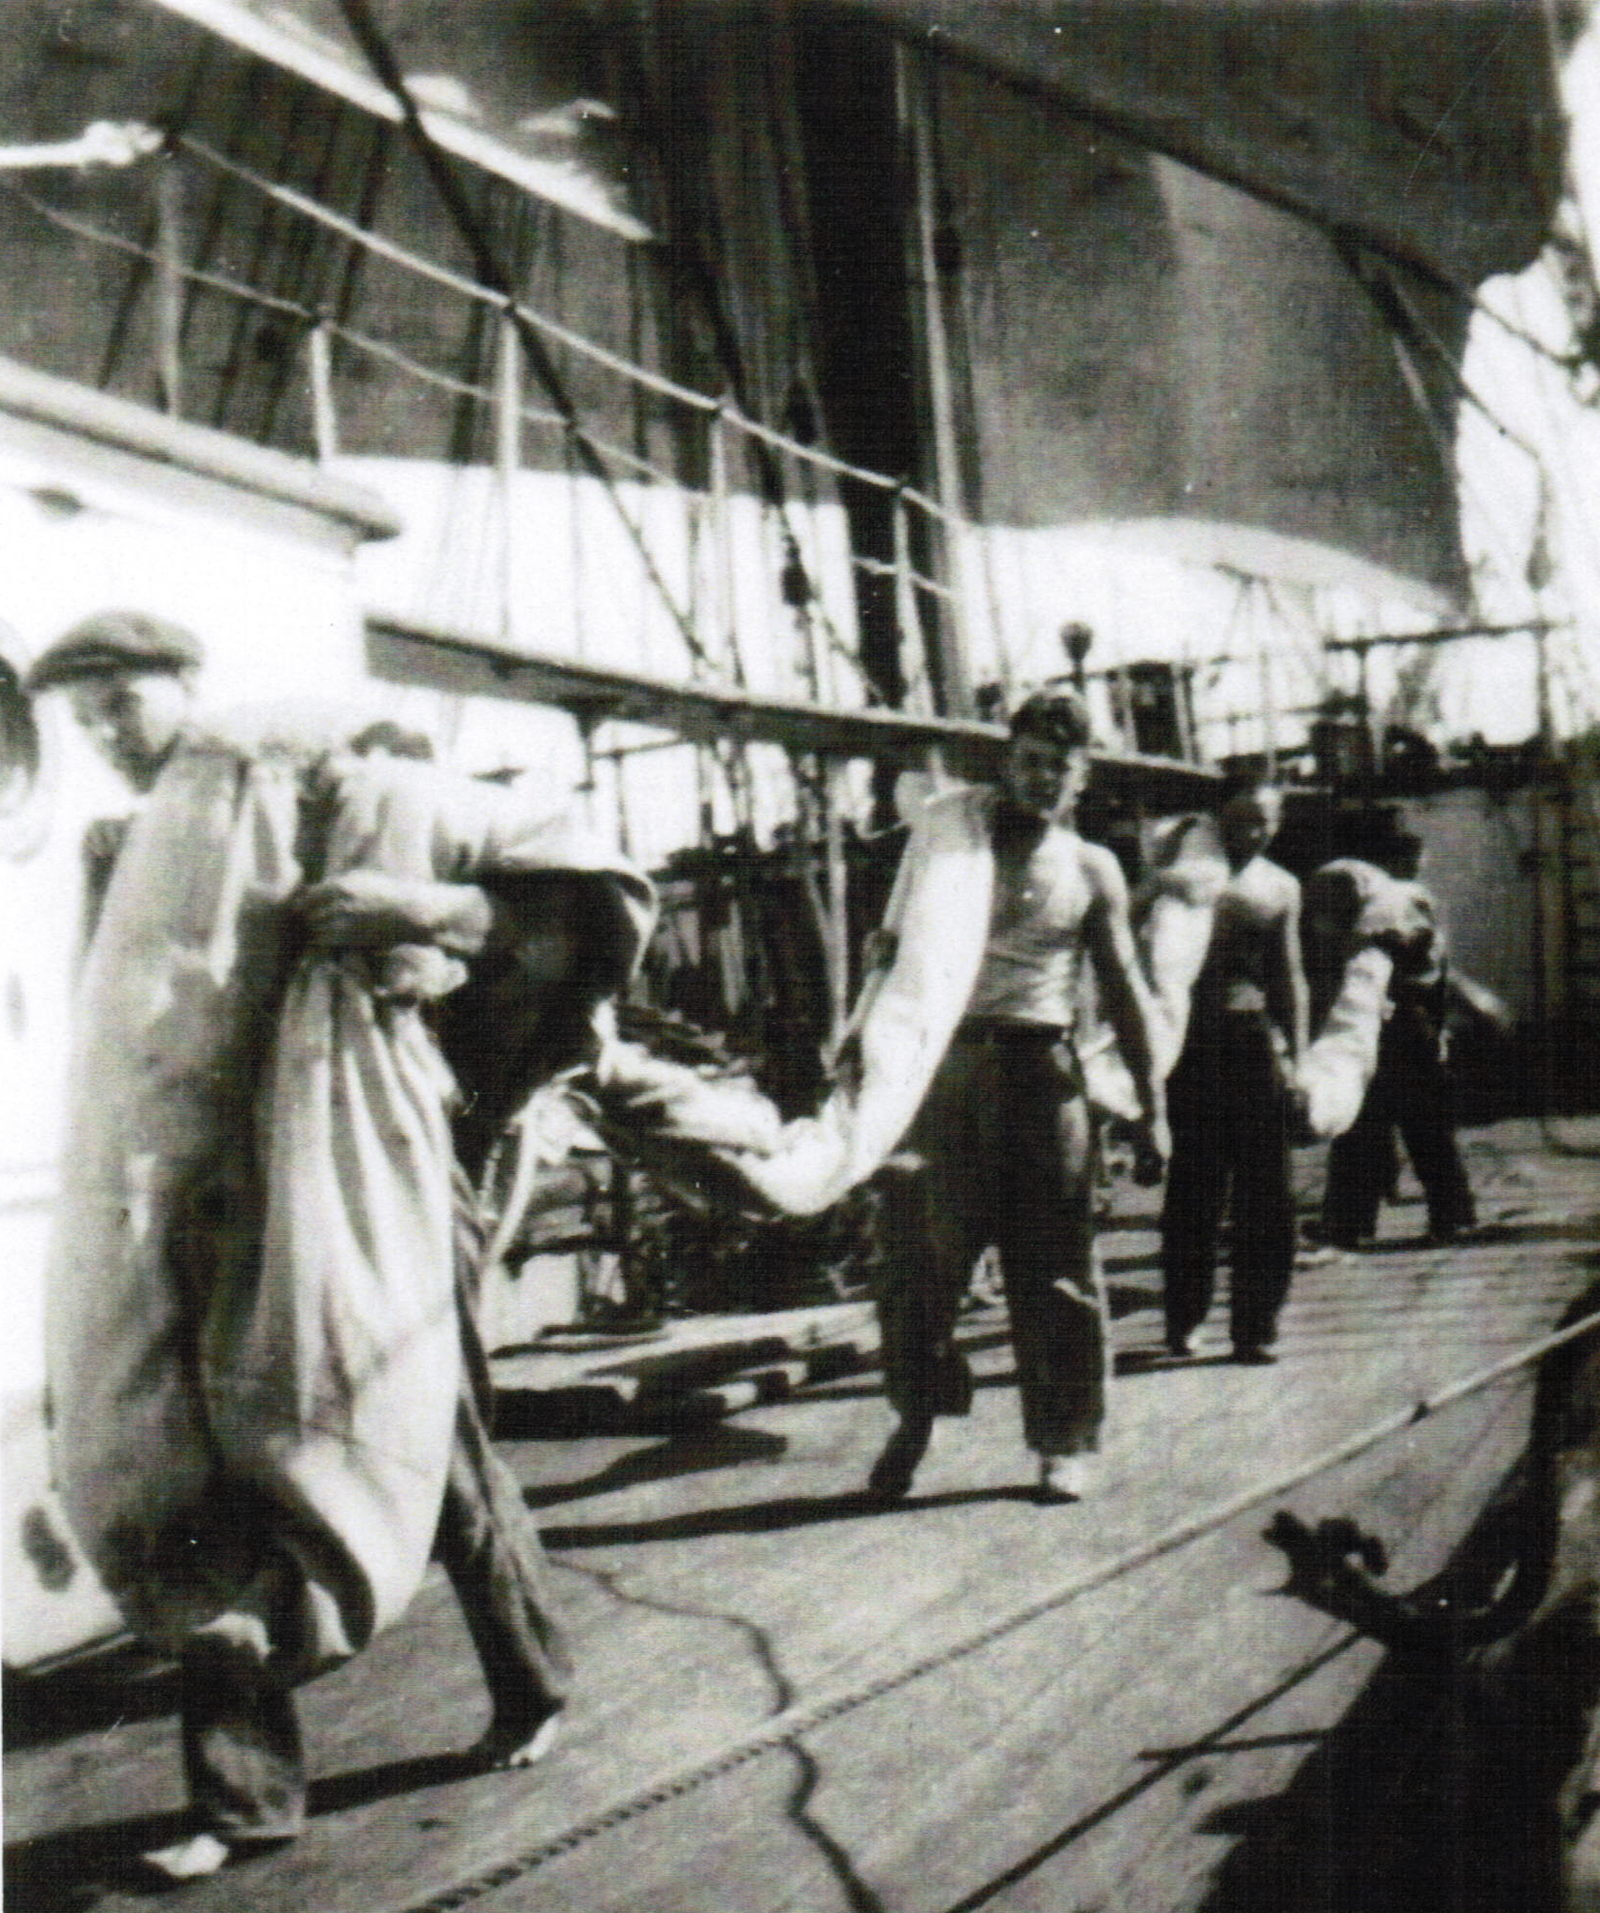
\includegraphics{./images/image022.png}
\caption{(Unlabeled)}
\end{figure}

\hypertarget{thursday-15th-june}{%
\section{\texorpdfstring{Thursday 15\textsuperscript{th}
June:}{Thursday 15th June:}}\label{thursday-15th-june}}

Bowling along with weather unchanged -- 8-10 knots.

Painting and chipping rust during morning. Early morning watch I had
1\textsuperscript{st} wheel and so was at Lookout at 6am but as was
Daylight came down. 2\textsuperscript{nd} Mate came up --looked at the
pigsty, looked further for Ayliffe or Philips (both free at coffee time
until 6.30) and after glancing first at me and switching back to pigsty
several times, suggested, almost apologetically, that I clean it out.

He has avoided giving me the filthy jobs of late, for some reason. Was
nearly caught aback when at wheel tonight at sudden veer of wind but got
her back O.K. Have a horror of being caught aback, having visions of the
dismasted `Huogomont' still vivid in my mind. Making 3° Northwards each
day and can no longer see the Southern Cross in the Southern Heavens.

Once past 18° South (going North) the Southern Cross disappears finally.
Steffan came up to Lookout with me tonight and yarned.

``You see new stars you haf neffer seen now'' and he pointed out them --
the brighter ones to me. ``There you see Venus -- very red you see. I
haf many times rang the bells I think it was steamer on the horizon.''

He is quite an authority on the constellation in the Heavens.

\hypertarget{friday-16th-june}{%
\section{\texorpdfstring{Friday 16\textsuperscript{th}
June:}{Friday 16th June:}}\label{friday-16th-june}}

Braced this morning -- now ``Fuel \& by'' -- noticed the difference when
bracing with the smaller personnel of the watch -- perfect weather.

\hypertarget{saturday-17-june}{%
\section{Saturday 17 June:}\label{saturday-17-june}}

Making same steady progress Northwards.

Changed all sails on Foremast today -- starting with the Royal.

Feeling very fit.

The work aloft is glorious in this weather. I searched the horizon for
steamers in vain.

\hypertarget{sunday-18th-june}{%
\section{\texorpdfstring{Sunday 18\textsuperscript{th}
June:}{Sunday 18th June:}}\label{sunday-18th-june}}

Another day in flawless weather. This is the life!

We are braced somewhat differently now we are in the Trade winds -- the
Royals almost square and the courses braced fairly hard up. So although
the wind may veer 1 or 2 points bracing is not necessary. Tonight All
Hands gathered on the Main Hatch lying on spare sails and indulged their
musical talents -- such as they are in uproarous chanties and songs.

\begin{figure}
\centering
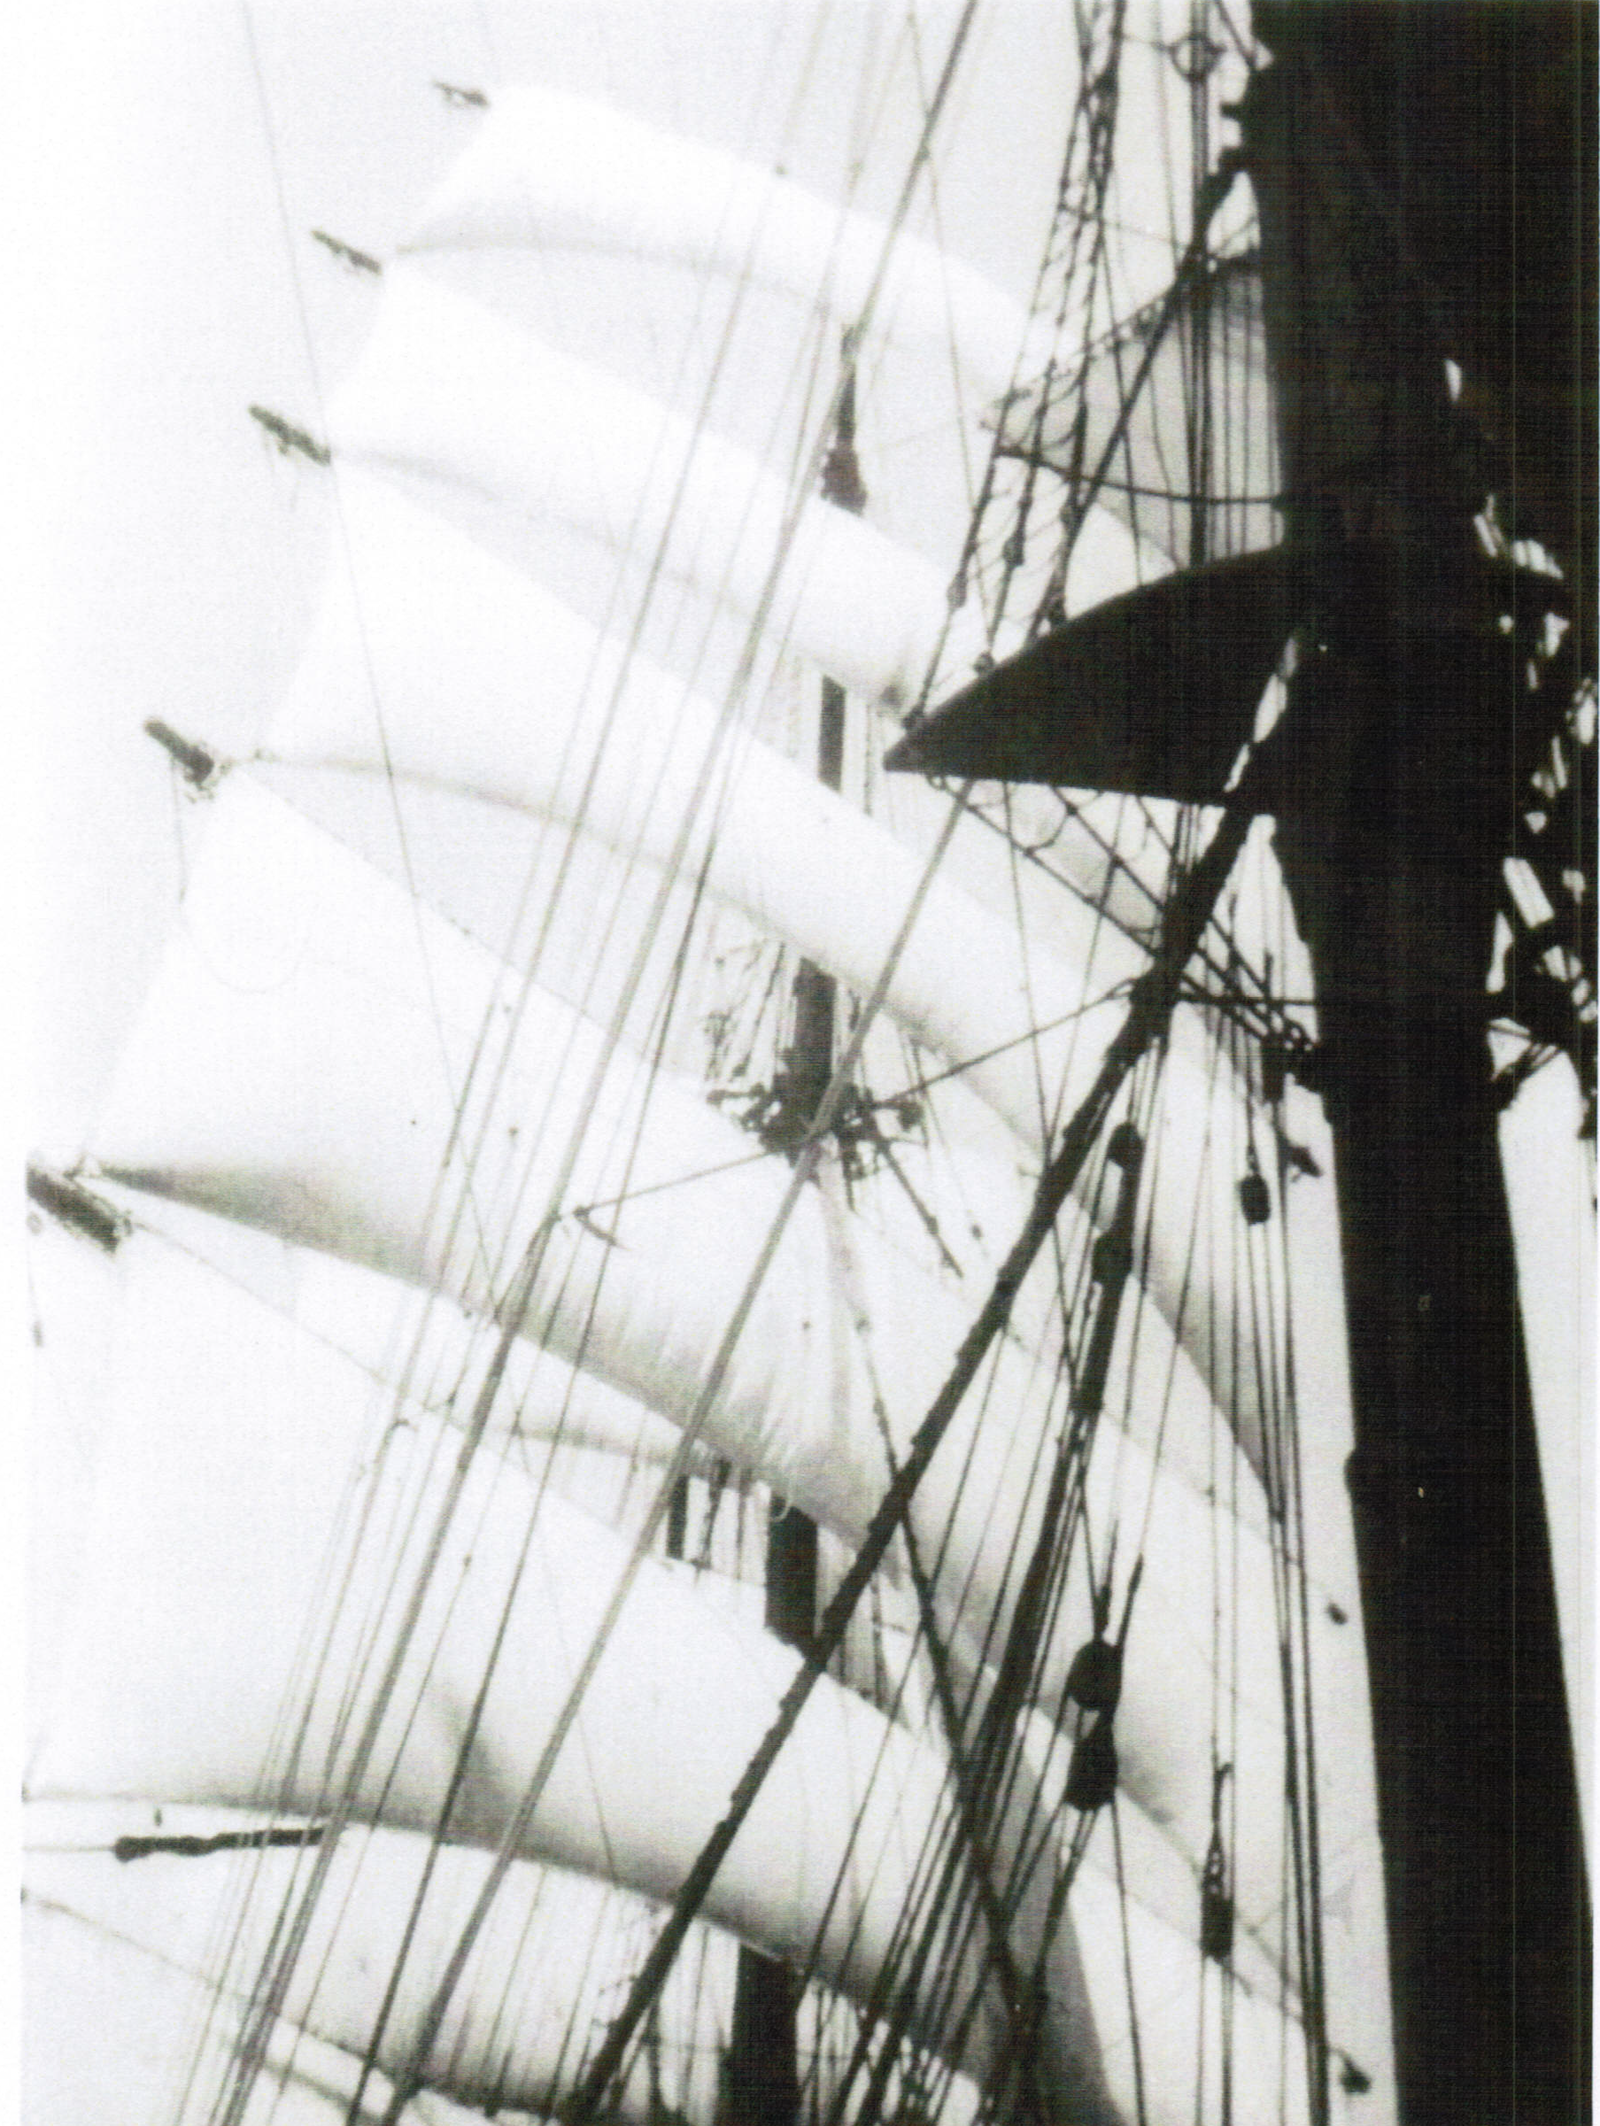
\includegraphics{./images/image023.png}
\caption{``Those glorious S.E. Trade winds''}
\end{figure}

The versions of the majority being necessarily omitted from our
conventional Song Books.

``Maid of Amsterdam'', Rolling down to Rio; Around Cape Horn in 90 Days;
Billy Bay and countless others -- with perhaps the ``Tinkers Song''
taking pride of place even with the Finns.

It was a perfect evening -- the warm mellow breeze -- the ship ghosting
silently thro' the water -- above the massive spars, yards and mast and
rigging thrown into pleasing relief

against the starlit sky and those great masses of billowing sail
appearing in the moonlight to be carved from marble. Gradually the
singing dies away -- we meditate with our pipes and finally sleep.

\hypertarget{monday-19th-june}{%
\section{\texorpdfstring{Monday 19\textsuperscript{th}
June:}{Monday 19th June:}}\label{monday-19th-june}}

We are all very happy and contented with our lot, for which I think the
weather is largely responsible.

I think we would all be happy to go on sailing like this forever\ldots!

How man changes with his environment.

Bent on new Cro'Jack today and when free we set about catching rates --
the only real amusement on board. A plate is secured, filled with rum
and placed on the wheat in the hold. (Hatches now opened). Along come
the rats sniffing -- we have also placed a lantern below and can see
everything going on. They have a quick drink of the rum, that terrible
potent Fire water, and go away about 6 ft -- return and have another
drink. It is now safe for us to descend into the hold and although in
full sight of the drunken rats they CAN NOT RESIST HAVING MORE RUM AND
RETURN TO THE PLATE for more.

They are then quickly dispatched to their cheesy Heaven!

But it's funny to see them look up at your -- quite drunk and not a bit
afraid -- `Dutch' courage! We are now washing the decks down every night
to prevent the planking shrinking and warping in the heat of the day.

\begin{figure}
\centering
\includegraphics{./images/image024.png}
\caption{Free Watch. On 2\textsuperscript{nd} Sunday at sea. We catch an
Albatross. Rutherford, self, Phillips, Busthelm, Steffan}
\end{figure}

\hypertarget{tuesday-20th-june}{%
\section{\texorpdfstring{Tuesday 20\textsuperscript{th}
June:}{Tuesday 20th June:}}\label{tuesday-20th-june}}

We are now at latitude 3°20.5 -- about 3 1/2° N to go and we cross the
Equator and on to Stage two of our voyage. The weather is now typical of
the Doldrums -- the atmosphere inclined to be sultry and hot, but not
unpleasantly so. The sea water is quite warm and we lower ourselves over
the side for a swim at night -- this strictly forbidden, but \ldots..

Last night Paul slept on Police and the whole watch called out and
warned that the next time it occurred would be the last and thereafter
the whole watch would be forced to remain on deck during night watches.
The breeze dropped very light at midnight, fickle airs coming from all
points of the compass but after 2 hours the breeze came again and
slightly stronger as if guilty and wishing to make amends for leaving
us. We slept free watch on deck

\begin{figure}
\centering
\includegraphics{./images/image025.png}
\caption{Rutherford}
\end{figure}

\begin{figure}
\centering
\includegraphics{./images/image026.png}
\caption{Steffan cuts Ayliffe's hair}
\end{figure}

\hypertarget{wednesday-21st-june}{%
\section{\texorpdfstring{Wednesday 21\textsuperscript{st}
June:}{Wednesday 21st June:}}\label{wednesday-21st-june}}

The crew are informed that we have another man amongst us -- Coventry
being 21 today. Celebrations to be held Sunday next. We expect to pick
up the S.E. Sister winds, the North East Trades soon but present breeze
is still very favourable on the quarter. The days pass as most days do
in this weather -- quickly and pleasantly.

An amusing incident occurred late this afternoon concerning Rutherford.
He was working on deck and four men aloft were using him as a messenger
boy to bring them tools they had forgotten. Now climbing the rigging is
alright once, tolerable twice but the third time he rebelled and
shrieked back in a fury, curses which with his newly acquired knowledge
of Swedish oaths, blended with a highly creditable number of Australian
masterpieces, caused the mate to gaze at him with obviously mixed
feelings of admiration and envy.

Invoking ``Saaten'' three times in rapid succession he concluded in a
hoarse voice ``What the hell do you think I am, a b\ldots\ldots y ape?''
The day finished with the crew fishing and rat catching. Lookout late
tonight was a revelation; I have read of ships ghosting along but
tonight could really appreciate just what the implied. I serenaded the
Stars! And so we ghost on silently until on

\hypertarget{thursday-22nd-june}{%
\section{\texorpdfstring{Thursday 22\textsuperscript{nd}
June:}{Thursday 22nd June:}}\label{thursday-22nd-june}}

Between 6 am and 6.30 am we ``Cross the Line''. Contrary to expectations
we do not get a holiday.

During the freewatch we set fishing lines and catch two fish of the
mackerel family -- a beautiful streamlined fish with retractable upper
and lower fins; the skin hard and leathery and almost devoid of scales.

They appear capable of great speed. Flying fish also very numerous. Most
difficult to stay awake during night watches. Writing this diary is main
occupation, but tonight I went to extremes to stay awake -- necessary
extremes. I paced the deck, tried singing, washed, drank lime juice, but
was still horribly drowsy. At length I snatched a blanket and went
for'ard on the fo'castle head, told Lookout to waken me in the event of
any whistles being blown and slept until 5 am.

The wind dropped just before daylight and on

\hypertarget{friday-23rd-june}{%
\section{\texorpdfstring{Friday 23\textsuperscript{rd}
June:}{Friday 23rd June:}}\label{friday-23rd-june}}

We find ourselves almost becalmed.

However at midday a light breeze arrived and we brace.

We had almost finished bracing when Phillips came dashing aft shrieking
``Steamer -- Steamer''. Within 30 seconds the whole crew, from Captain
to Cook, were leaning over the lee (Port{]} rail and gazing over the
fore quarter, where the two masts of a Steamer could be just seen in
relief against the horizon. Having just previously been told aloft to
overhaul buntlines, I quickly lay aloft and made out the grey hull of a
Steamer some 5 miles distant to lee and apparently hove to. We alter
course but in the light breeze barely make 3 knots -- the crew pace up
and down impatiently and suddenly there comes a cheer. The other boat
has turned and is steaming fast straight to us. The Captain and mates
dash about sorting signal flags, whilst the crew argue about the
Nationality of the other vessel.

Much speculation goes on -- until finally she rounds up -- we read
``Argentina'' Stockholm on her stern. So she's Swedish -- and a neat
ship too -- motor ship -- Diesel driven.

The signals fly fast -- we learn that Europe is in Peace, check the
Chronometer and position -- request her to report us to Lloyds and after
the first awed silence, cheer her enthusiastically.

Suddenly our chaps give another frantic cheer -- a few girls have
appeared on deck and are waving scarves and handkerchiefs Gosh are the
mob making a row -- whistling -- ``see you in Stockholm'' etc.

Freddie and Turipa look at the girls -- look at the water between the
two vessels, scratch their heads and mutter ``Saaten, saaten''. Past us
she rushes and with a final cheer veers off and resumes her course. Much
discussion goes on and no work' we all are grinning and feel like
slapping each other on the back.

I was at wheel 3-4 pm when suddenly the 2\textsuperscript{nd} mate
rushed up, snatched the telescope and there, behold, another Steamer on
the horizon aft. However she finally dipped and disappeared about 1 ½
hrs later, amid our curses.

Ah well, one Steamer to talk in one day is another!

And next Monday in Lloyds gazette will appear ``M.V. Argentina'' spoke
Barque ``Archibald Russell'' -- Lat 2°23.9 N Long 29°27.6 W, X days from
S.Australia. Heavy rain tonight.

\begin{figure}
\centering
\includegraphics{./images/image027.png}
\caption{Our first Steamer: M.V. ``Argentina''}
\end{figure}

\hypertarget{saturday-24th-june}{%
\section{\texorpdfstring{Saturday 24\textsuperscript{th}
June:}{Saturday 24th June:}}\label{saturday-24th-june}}

Raining and we are becalmed. It would!! Today you see is full Holiday --
``Midsummer day'' Free night tonight -- only risen up 4 times between 9
pm and 4 am -- good going.

\hypertarget{sunday-25th-june}{%
\section{\texorpdfstring{Sunday 25\textsuperscript{th}
June:}{Sunday 25th June:}}\label{sunday-25th-june}}

Weather cleared and with the sun right overhead, as hot as fire. Breeze
picked up from aft -- 4-5 knots.

Tonight wind fell off again -- we clew up the courses.

The subject of tonight's furious argument ``The Safety of travel by
Steamer as compared with travel by Sailing vessel''. Results about
50-50.

\hypertarget{monday-26th-june}{%
\section{\texorpdfstring{Monday 26\textsuperscript{th}
June:}{Monday 26th June:}}\label{monday-26th-june}}

An absolute flat calm and by God it's hot.

A shark circles around the stern of the ship which Tria and the
Donkeyman attempt to catch -- unsuccessfully. By 9.30 temperature 98°F
and rapidly getting hotter.

Wheel, which I took from 9-10 am, was an ordeal. Sailing ``By the
wind''; you look up for an hour at those upper sails, made an eye
burning white by the sun. The rays from the sun also come pouring thro'
the Porthole immediately above your head and the metal wheel house, too
hot to touch, sends out searing waves of heat to complete the baking.
You stand there steering, sweating and swearing and at the end of the
hour step out of the puddle of perspiration at your feet. I leave the
wheel and check up on the temperature -- 102°F -- on the sea and in the
humid tropics.

Yes its hot!

Then to painting \& scraping-exposed to the sun of course

Drinking water warm; everything's warm. Damn!

We come off watch feeling very disgruntled to Salt Buffalo and peas for
dinner.

Suddenly thro' the skylight a puff of wind comes, cool and pleasant.
Within half an hour a good N.E. breeze has worked up with tropical
squalls and rain and we surge along 6-8 knots braced up hard on the
Starboard tack. Everybody talking N.E. Trades. How we hope!

At 2.30 I hear from my bunk where I write my diary, the crack and loud
reports of a blown sail -- the 1\textsuperscript{st} and
3\textsuperscript{rd} mates' voices sound urgent. It's a squall and she'
groaning and quivering under the pressure of full sail -- burying her
lee rail far under.

I dash for'ard to see the Fore Upper T'Gallant blown to hell and pieces
of sail careering over the sea. Its `up aloft and make fast' and six men
string out along the yard and take in what's left of the sail. The masts
are heeling far over the sea making progress aloft easier. Two berets go
howling away to lee -- torn off by the wind; their owners pause for an
instant to curse.

I climb around aloft, camera slung around my neck and finally obtain
several good shots. Within ½ an hour wind eases and we steady at 8
knots.

\hypertarget{tuesday-27-june}{%
\section{Tuesday 27 June:}\label{tuesday-27-june}}

Flying fish still accompanying us in large numbers. Their grace and
speed in flight is very fascinating to watch. These are the N.E. Trade
winds without a doubt -- we surge steadily along at 7 ½ knots with the
weather much more pleasant. The ship is becoming ship shape slowly --
the painting is making a vast improvement in the appearance and when we
reach Port she should look great. When!!!

\hypertarget{wednesday-28-june}{%
\section{Wednesday 28 June:}\label{wednesday-28-june}}

Weather unchanged -- making 2° Northwards daily. With the hatches off,
rats are becoming a pest -- they are even invading our fo'castle.

Thursday June 29\textsuperscript{th}

Still plugging along steadily. Was at wheel 6-7 pm tonight when shackle
on Mizzen Royal sheet snapped with a loud crack -- like a pistol shot. I
thought the T'Galant mast was coming down -- it swayed horribly, but the
mate lowered the yard in time. He was quite pale afterwards -- he too
thought the mast was coming down.

Steffan made fast the sail.

Friday June 30\textsuperscript{th}

Sheet and shackle repaired on Mizzen Royal and sail set again. Now on
level latitude with Cape Verde Islands.

Sighted steamer which crossed our bows well away, going West to East.
Still rolling Northwards -- life is a yachting cruise these days.

\hypertarget{saturday-1st-july}{%
\section{\texorpdfstring{Saturday 1\textsuperscript{st}
July:}{Saturday 1st July:}}\label{saturday-1st-july}}

Another good day with wind strengthening. Tonight all Hands muster aft
and demand to see the Steward.

Stanlund and Timpa (brothers) acting as spokesmen angrily demand better
food and hot words rock back and forth but as usual nothing further is
done about it. For a short while after 4 bells (10 pm) the wind
strengthened hard and we tore thro' the water 12-14 knots with the rail
constantly disappearing beneath the boiling foam. The deck was at such
an angle that it was almost impossible to walk it.

The old sails rip and tear but hang together and daylight reveals many
great holes.

\hypertarget{sunday-3rd-july}{%
\section{\texorpdfstring{Sunday 3\textsuperscript{rd}
July:}{Sunday 3rd July:}}\label{sunday-3rd-july}}

I practice wire splicing and sail sewing and make letter satchel.

\hypertarget{monday-3rd-july}{%
\section{\texorpdfstring{Monday 3\textsuperscript{rd}
July:}{Monday 3rd July:}}\label{monday-3rd-july}}

Wind swings two points more East -- is it the end of the N.E. Trades?

We clear out our fo'castle and begin painting and scrubbing thoroughly.

This necessitates sleeping on deck and I bunk on Main Hatch with
Steffan. Some of the crew sleeping in the Hold on the bags of wheat but
after seeing two rats chased from one bunk, I decided to risk a rain
squall and brave it on deck. However at 3.45 am on

\hypertarget{tuesday-4th-july}{%
\section{\texorpdfstring{Tuesday 4\textsuperscript{th}
July:}{Tuesday 4th July:}}\label{tuesday-4th-july}}

Seven of us were caught by a sudden rain squall. The others dashed aft
under the break of the Poop, but after a glance at the sky, I decided to
stay, as it did not appear more than passing shower and so it turned
out.

Crossed Tropic of Cancer last night -- 23 1/2° N and so emerge from
Tropics. Wind very puffy but still quite strong.

\hypertarget{wednesday-5th-july}{%
\section{\texorpdfstring{Wednesday 5\textsuperscript{th}
July:}{Wednesday 5th July:}}\label{wednesday-5th-july}}

Not a cloud in the sky and wind very light. Thus the N.E. Trades die
away.

We paint ship and argue how many more days to England -- we run a
sweepstake on it.

\hypertarget{thursday-6th-july}{%
\section{\texorpdfstring{Thursday 6\textsuperscript{th}
July:}{Thursday 6th July:}}\label{thursday-6th-july}}

Becalmed! The N.E. winds have finally deserted us and we lie clewed up
in the Doldrums -- the Horse latitudes.

Food terrible -- salt Buffalo every day and brown beans. Very hot. We
now wait for the prevailing ? West winds.

\hypertarget{friday-7th-july}{%
\section{\texorpdfstring{Friday 7\textsuperscript{th}
July:}{Friday 7th July:}}\label{friday-7th-july}}

Flat calm. We swear. This morning a large shark was seen lazing around
the stern of the ship and we promptly put out a line.

The two striped Pilot fish -- parasites that live on the shark itself --
left the shark and after inspecting the bait swiftly returned to the
shark and guided it to the hook, where it snapped simultaneously with
the linesman's pull. All Hands hauled the shark out of the water -- we
quickly passed another loop-line around the threshing tail. We just
finished this when the hook parted from the line and the shark was
suspended ½ in and ½ out of the water -- head down.

After much struggling at both ends of the line around the tail we get it
aboard, stun it with Capstan bars. Ten minutes later barely a bone is
left in the carcass.

The opening up revealed 5 perfectly formed young sharks which as soon as
released struggled hard.

We tossed one over and away it swam in great style -- keeping around the
ship. The heart of the mother shark was still beating some hours later.
Perfect night -- but still no wind.

\hypertarget{saturday-8th-july}{%
\section{\texorpdfstring{Saturday 8\textsuperscript{th}
July:}{Saturday 8th July:}}\label{saturday-8th-july}}

Gentle drift of air from S.W. this morning -- about 1 ½ knots. Very hot
-- clear sky.

The carcass and blood from the killed shark has evidently attracted
others, as we count a score of dorsal fins cruising about 100 yds astern
-- but we still have our evening swim.

\hypertarget{sunday-9th-july}{%
\section{\texorpdfstring{Sunday 9\textsuperscript{th}
July:}{Sunday 9th July:}}\label{sunday-9th-july}}

No wind -- but we move almost imperceptibly forward with the drift at
about 1 knot.

We braced 4 times during day to catch every little rare puff -- it is
terrible work in the heat.

Rutherford failed to rise up at 8 bells (8 am) this morning and
Starboard watch helmsman kept waiting 10 minutes at wheel. Paul, who had
woken Rutherford, abused him and cursed the Port watch generally, when
Hanlon came on the scene and took up the argument for the Port watch and
in turn, abused the Starboard watch. The argument rapidly became
personal and Paul, becoming enraged, like a flash knocked Hanlon to the
deck with a terrific blow to the head. Hanlon was dazed for a few
seconds but he's certainly got ``guts''. Built lightly and possessing
nothing of Paul's magnificent physique, he came back furiously, and by
clever hitting and dodging crashed Paul into the pin rail.

However, by this time, being the nearest to them, I thought it best to
end the unpleasantness and with the aid of a belaying pin separated
them. Both stalked off in a fury. This goes to show what state of mind
we are in -- 97 odd days at sea and sick of each other -- intolerant and
generally grumpy. And yet we might one minute be yarning pleasantly
together and the next minute \ldots.

\begin{figure}
\centering
\includegraphics{./images/image028.png}
\caption{Hanlon Coventry. Scrubbing teak in cold weather. (Note Hanlon's
hand in pocket.)}
\end{figure}

\hypertarget{monday-10th-july}{%
\section{\texorpdfstring{Monday 10\textsuperscript{th}
July:}{Monday 10th July:}}\label{monday-10th-july}}

Bent on new sails on Foremast and main mast -- replacing Trade sails.
Had foul time going to peak right to the truck of the Foremast,
unlashing a heavy block and going to deck and then taking it to the
truck of the Mainmast. The weight of the block caused the rope around my
shoulders to tear the skin and I was bleeding freely when I ultimately
returned to the deck. This brought about my first argument with the
2\textsuperscript{nd} mate --honours about even.

Weather exhausting -- over 100°F.

Moved back into our freshly painted fo'castle today.

\hypertarget{tuesday-11th-july}{%
\section{\texorpdfstring{Tuesday 11\textsuperscript{th}
July:}{Tuesday 11th July:}}\label{tuesday-11th-july}}

A light breeze from North -- we tack ship at 8 bells during morning
watch. Wind swings again an hour later and we tack ship once more.

Heartily tired of calms and praying for a blow -- we have made
practically no progress for a week.

Tonight I was free but at 3.30 am two whistles go -- out I go in shorts
to find the ship flat aback and rain pouring down.

Only 4 of the watch turn out -- McRae and Steffan were not woken by
Ayliffe (Police) (actually not supposed to be asleep) and the
2\textsuperscript{nd} mate, already in a rage with the helmsman, dashes
off to find them. We, Haula and I, find Steffan for'ard and,
unfortunately, the mate found ``Mac'' aft.

He shook him, and as soon as ``Mac'' sat up, struck him on the face
hard. ``Mac'' grabbed the mate's arms and held on and then all Hell let
loose.

Hearing the yells and curses, we dash aft, Haula arming himself with a
belaying pin, as soon as we come on the scene, the mate jumped for the ½
deck companionway and safety, where he reviled us as never before in a
voice vibrant with passion.

God! What a temper!

``Mac'' usually so quiet was not at his best on being so suddenly
awakened and on an empty stomach and he gave as good as he got. However,
the ship aback, we cannot afford to waste time arguing and the whole
watch, muttering angrily, go to the braces.

The Skipper suddenly appears and a deadly quiet reigns.

Eight bells, 4 am, change of watch we go below. Since in the fo'castle
the watch decide the course to be followed the next occasion the mate
attacks any member and as ``Mac'' said ``He'll get his!''

\begin{figure}
\centering
\includegraphics{./images/image029.png}
\caption{L.R. Self, Paul (white cap), Kannianann, Ayliffe, Donkeyman,
Weronan, Bos'n}
\end{figure}

\begin{figure}
\centering
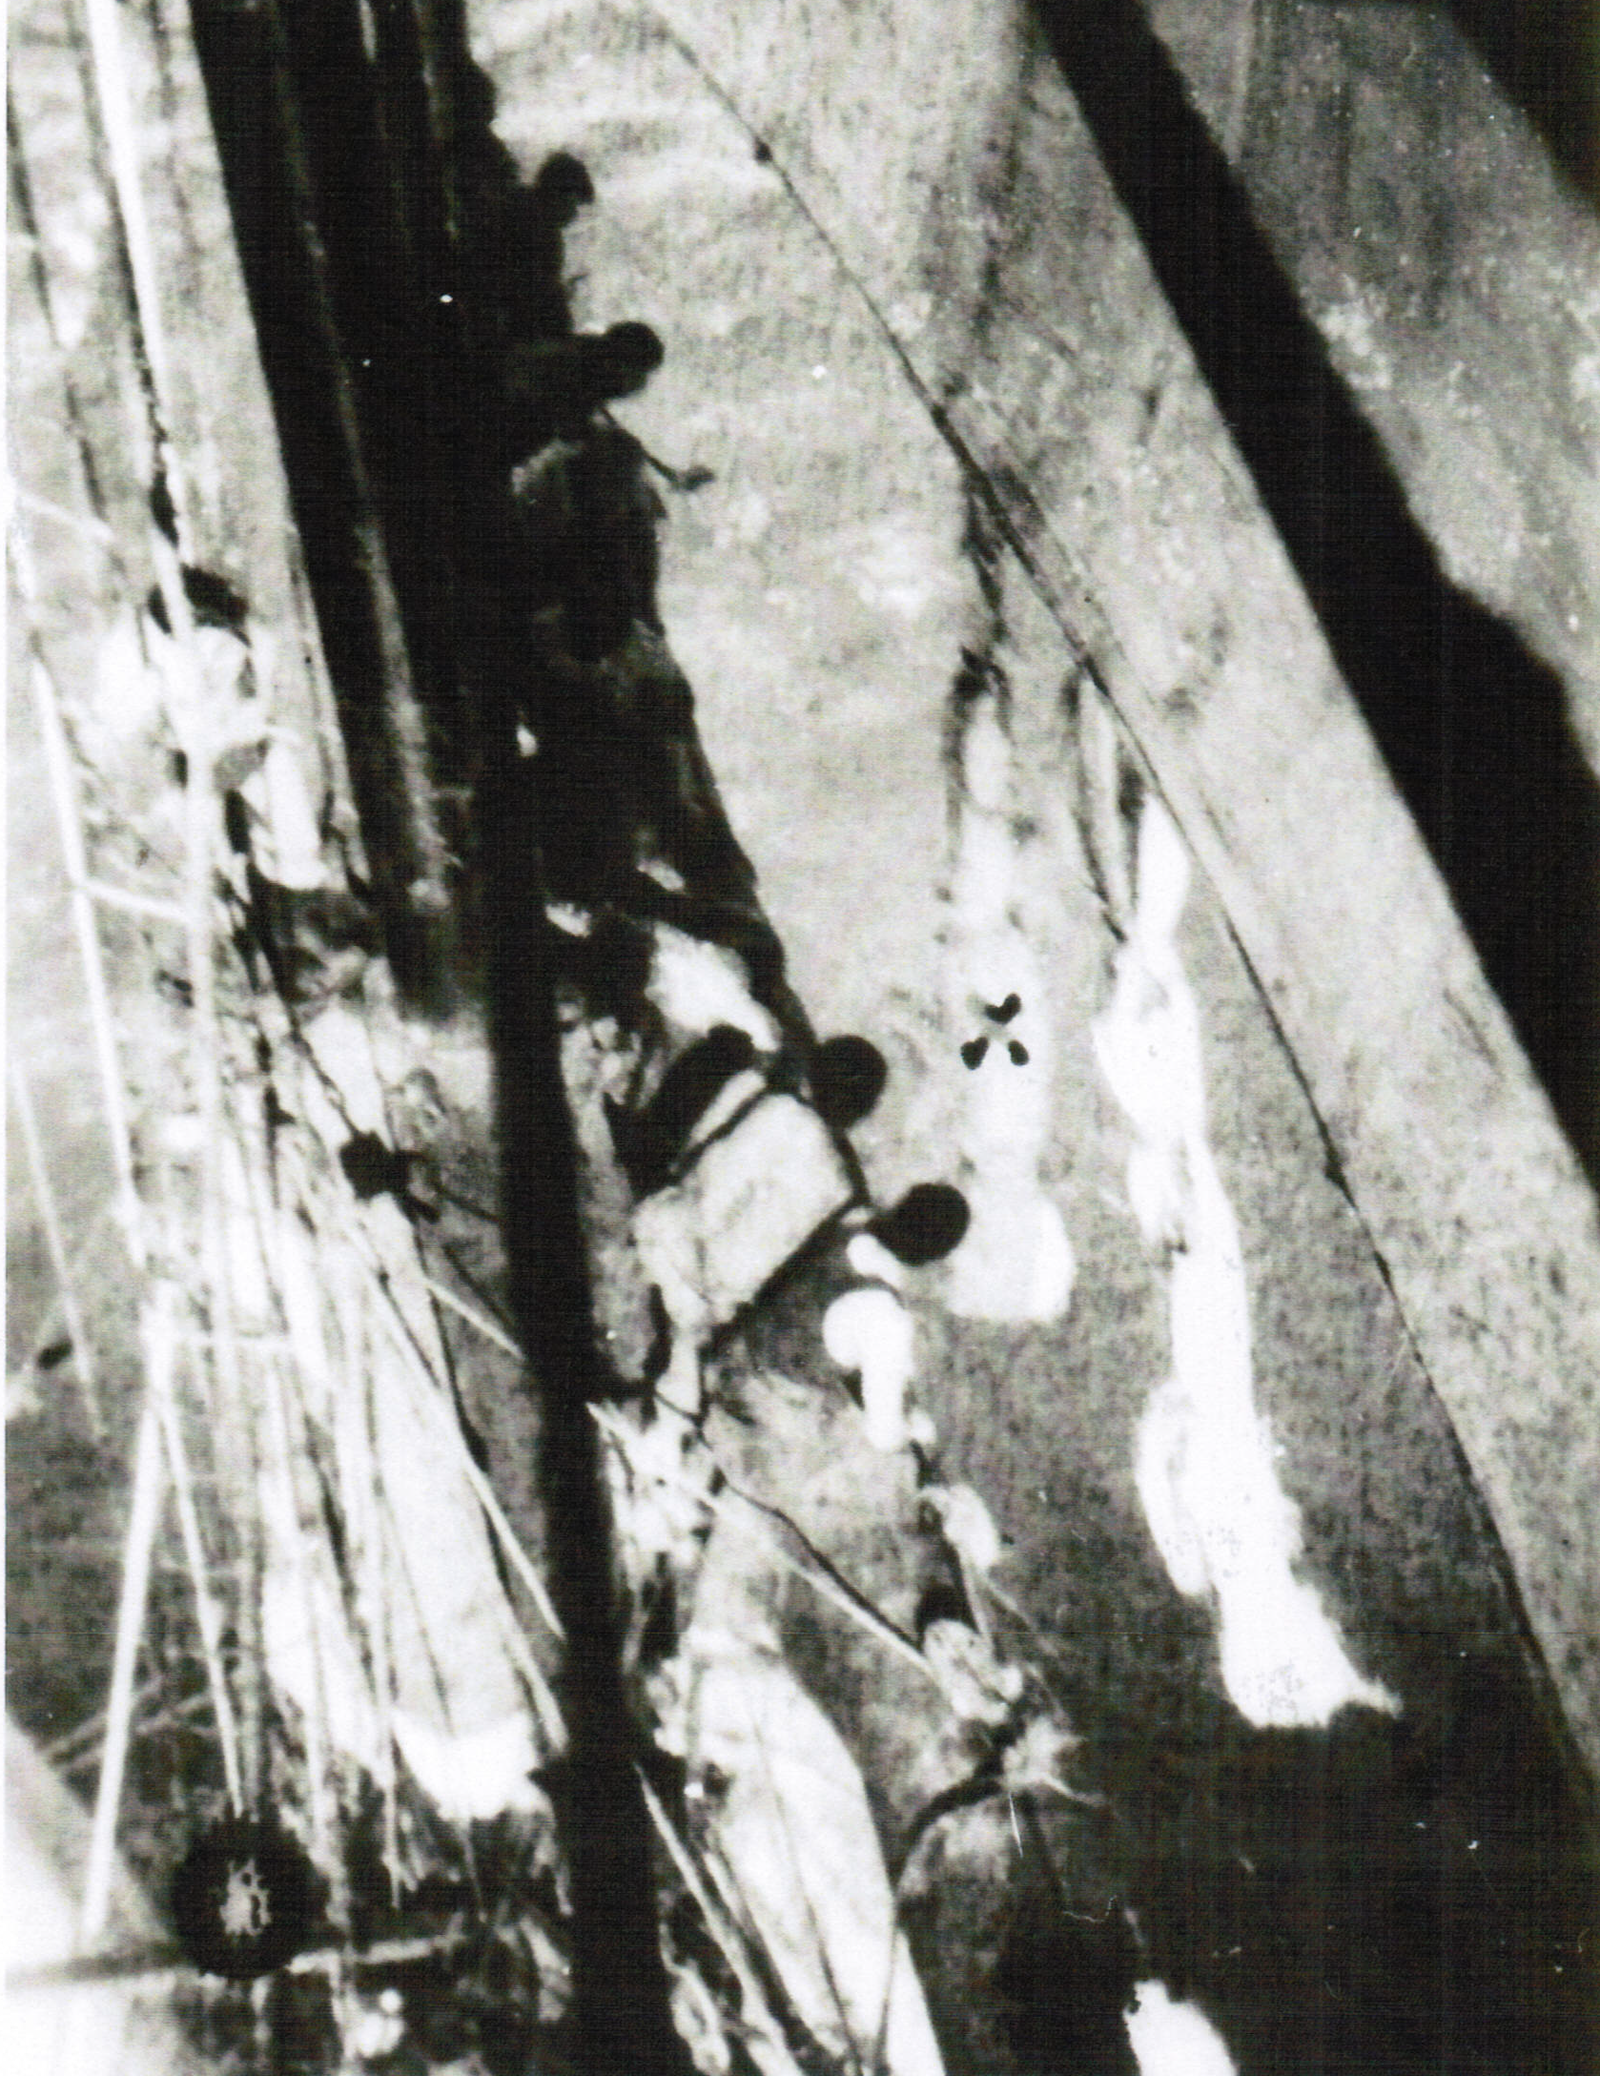
\includegraphics{./images/image030.png}
\caption{Hauling a shark aboard}
\end{figure}

\hypertarget{wednesday-12th-july}{%
\section{\texorpdfstring{Wednesday 12\textsuperscript{th}
July:}{Wednesday 12th July:}}\label{wednesday-12th-july}}

One hundred days at sea.

We tack ship twice during the morning but wind very light and fluky that
we make no progress.

Once whilst in the middle of tacking operations the wind died and we are
left in ``Irons''.

Crew discussing the incident of last night -- it appears that the best
course is to wait until Port is reached -- at sea such action is or
could be taken as mutiny unless it could be definitely established that
the mate attached first -- which thus far has been the case on each
occasion. This being our ninth day of calm we decide we have a ``Jonah''
amongst us.

The Sailmaker (industrious bloke!) accordingly drew up 19 pieces of
paper -- one having ``Jonah'' written on it. We each draw a slip at a
gathering of ``All Hands'' in the big fo'castle.

Poor old ``Mac'' was unlucky enough to draw the dreaded slip and looked
quite embarrassed about it.

\hypertarget{thursday-13th-july}{%
\section{\texorpdfstring{Thursday 13\textsuperscript{th}
July:}{Thursday 13th July:}}\label{thursday-13th-july}}

An entire absence of wind, bringing on sultry stifling heat. Slight
breeze from aft midday -- we square up hopefully, hardly daring to
breathe.

This afternoon saw a shoal of whales, at least a dozen, probably far
more of them, swimming and larking about in the water 200 yards away.

\hypertarget{friday-14th-july}{%
\section{\texorpdfstring{Friday 14\textsuperscript{th}
July:}{Friday 14th July:}}\label{friday-14th-july}}

Wind drops light again midDAY 1 ½ knots. Sighted masts and funnel of
steamer some 10 miles away on our Port bow but too great a distance away
to distinguish Nationality, even thro' telescope. For the past week we
have been passing thro' weed from the Sargasso Sea off the Bay of Mexico
-- carried North by the currents. The weed contains many shells and
small pink crabs.

Tonight we are treated with a brilliantly vivid electrical storm, such
as only the Tropics can provide. From the time between the flashes and
the thunder we estimate the centre of the disturbance to be some 5 miles
distant.

With the grotesque formations of clouds in the sky and our sails and
rigging thrown out sharply in the flashes and the rolling of the
thunder, the scene is awe inspiring.

\hypertarget{saturday-15-july}{%
\section{Saturday 15 July:}\label{saturday-15-july}}

11 am steamer sighted coming up from aft. We alter course and signal and
slowly she comes up and passes us 100 yds to Port -- signals flying fast
the while. A British tanker, the ``Oliven'' of London and we -- the
Britishers -- cheer. Conversation is possible in the absence of wind and
we answer their enquiry ``103 days out'' -- ``bound for the Lizard or
Falmouth for Orders''.

We request them to send photographs which they are busy taking. They are
to report us to Lloyds and wishing us a happy voyage steam away.

She (Oliven) is a British Tanker -- Royal Navel Reserve crew -- denoted
by their Blue ensign with gold anchor inscribed. They can carry no
foreigners in crew.

\begin{quote}
Note: On reached Falmouth, I met the 2\textsuperscript{nd} Engineers and
the Wireless operator and we obtained negatives of photographs --
excellent copies. Had a yarn over beer. Killed a pig today in spite of
the heat. Wind dropped flat again and we lie motionless with drooping
sails and scorching decks.
\end{quote}

\hypertarget{sunday-16th-july}{%
\section{\texorpdfstring{Sunday 16\textsuperscript{th}
July:}{Sunday 16th July:}}\label{sunday-16th-july}}

An object sighted 5 miles away to Port -- we make out a boiler from a
ship adrift -- burst.

Whilst everyone gazing at this I saw from wheel a ship coming from
Starboard fore Quarter.

On her course she should pass about 400 yds ahead.

She is a Danish Tanker -- we salute and she returns the courtesy but
goes straight on.

Steffan and Bustholm jubilant at sighting a ship of their country.

Torrential rain tonight and very little wind -- we heave to.

Consumed colossal quantity of Pork today and had to sleep it off. This
after fast of 18 hours.

\hypertarget{monday-17th-july}{%
\section{\texorpdfstring{Monday 17\textsuperscript{th}
July:}{Monday 17th July:}}\label{monday-17th-july}}

Wind arrives about 5 pm and we steady at 5 knots close hauled.

\hypertarget{tuesday-18-july}{%
\section{Tuesday 18 July:}\label{tuesday-18-july}}

Wind at last. We stand ``full and by'' N.E. by E. at 8 knots. The
passenger is coming down to our fo'castle regularly each evening for a
yarn. The officers evidently ignore him -- showing none of the
courtesies due him and he has not been having a very pleasant time.

Their attitude seems to be one of necessary tolerance but this has led
him to fraternize more freely with us and he is proving a charming
companion.

\hypertarget{wednesday-19th-july}{%
\section{\texorpdfstring{Wednesday 19\textsuperscript{th}
July:}{Wednesday 19th July:}}\label{wednesday-19th-july}}

Wind and weather unchanged -- we paint all day. Reckon on 12-14 days to
England. Wind dropped 2 am on

\hypertarget{thursday-20th-july}{%
\section{\texorpdfstring{Thursday 20\textsuperscript{th}
July:}{Thursday 20th July:}}\label{thursday-20th-july}}

And we are almost becalmed. Sighted Steamer dead aft 11 am this morning
and she passes to weather close. A Danish Fruit boat, either from
Central American or Australia via Panama Canal.

\hypertarget{friday-21st-july}{%
\section{\texorpdfstring{Friday 21\textsuperscript{st}
July:}{Friday 21st July:}}\label{friday-21st-july}}

Fair progress -- N.E. by E. Lat 40.40N.

We work aloft chipping rust and oiling the metal chipped -- work on deck
almost completed.

Rain followed a 15 minutes squall tonight and then calm -- 2 knots.

\hypertarget{saturday-22nd-july}{%
\section{\texorpdfstring{Saturday 22\textsuperscript{nd}
July:}{Saturday 22nd July:}}\label{saturday-22nd-july}}

Midday wind allows us to make 8 knots. Sighted mast lights of large
steamer 11 pm tonight away to Port. She disappeared 4 hours later in the
darkness ahead.

\hypertarget{sunday-23rd-july}{%
\section{\texorpdfstring{Sunday 23\textsuperscript{rd}
July:}{Sunday 23rd July:}}\label{sunday-23rd-july}}

Wind strengthened and steadied -- we square up a little. The sky which
has been overcast for past 3 days has cleared and the sea is a beautiful
deep blue covered with sparkling white horses. This weather is very
refreshing and invigorating after the humidity of the Doldrums.

Glass dropping very low Tria informs us -- we expect some hard wind. On
going below 8 pm I quickly fall asleep and when awakened 12 midnight for
our watch from 12 to 4 am saw that the sky had become overcast and
covered with low and fast moving clouds.

Having first wheel woke me up properly -- the ship required handling
squall after squall but no rain.

1 pm I finished wheel turn and break into the galley and have a cup of
coffee and was just lighting pipe when a terrific puff hit the ship. The
masts and yards groaned and creaked above the whine of the wind as she
buries her lee rail and thunders thro' it at 14 knots.

Ten minutes later all is still again and suspecting rain I unpack my
oilskins. Thunder and lightening make the scene ominous and then down
comes the rain. One whistle -- that's Policeman and me and I cart water
for ½ an hr and then relieve Lookout 2 am to 3 am.

The wind lightened and we crawl along 4 knots. Visibility is limited
during the heavy rain to less than 50 yds but the discomfort of this
rain cannot be compared with rain in the West winds -- lacking the
deadly icy chill that numbs the whole body in a few minutes.

I pace up and down at Lookout thinking ``10 more days'' -- ``Ten more
days''.

Continually the whole ocean is lit by lightening which is not confined
to any one area but coming from all points of the compass. The thunder
seems only a ships length away.

Tonight I bet ``Mac'' 4 cigarette papers (worth about 5p) that wind will
swing to S.W. within 36 hours.

\hypertarget{monday-24th-july}{%
\section{\texorpdfstring{Monday 24\textsuperscript{th}
July:}{Monday 24th July:}}\label{monday-24th-july}}

A white capped wind disturbed sea and we rush along sailing splendidly.

Another steamer sighted ahead at 2 pm and passes ¼ mile away rolling and
pitching and taking over a lot of water.

The crew jeer ``Goddam Steambox''. She flies no flag and does not salute
us and we accordingly class her as a Dago or Greek Tramp.

Steamers are sighted almost daily now and although the chaps turn out to
look, there is not the wild enthusiasm of our first 2 or 3. Many eels
and turtles floating past carried North from the Bay of Mexico by the
Gulf stream.

\hypertarget{tuesday-and-wednesday-25-26-july}{%
\section{Tuesday and Wednesday 25 \& 26
July:}\label{tuesday-and-wednesday-25-26-july}}

Wind varying but we steadily make progress N.E. by E.

Becoming appreciably cooler, necessitating wearing a sweater.

Fog comes down when wind fell off.

\hypertarget{thursday-27th-july}{%
\section{\texorpdfstring{Thursday 27\textsuperscript{th}
July:}{Thursday 27th July:}}\label{thursday-27th-july}}

Sighted Steamer British Tanker ``Yarraville'' of Hong Kong. She's in
ballast and rolling and pitching. Salutes us as she rounds our stern and
we notice her ensign upside down -- signal of distress. However she
steams away again -- evidently some Chinese deck hand does not know how
to fly the British flag. I'll bet he was kicked from stern to stem for
his ignorance.

The Finns are smiling to themselves and inquire sarcastically ``New
British flag?'' ``Ar -- go and make yourself a square hat'' we reply
angrily.

But if we could just get at that man who sent up that flag -- just for 5
minutes\ldots.

By Gad -- it was humiliating!

Wind hard from S.W. and we log 10 knots for 4 hours -- grey sky and
drizzle -- grey-green seas -- big and much spindrift.

\hypertarget{friday-saturday-28th-and-29th-july}{%
\section{\texorpdfstring{Friday \& Saturday 28\textsuperscript{th} and
29\textsuperscript{th}
July:}{Friday \& Saturday 28th and 29th July:}}\label{friday-saturday-28th-and-29th-july}}

Wind drops. Confound the luck!

We make but 4 knots.

During the day we prepare ship for Harbour -- everything newly painted
and clean scrubbed decks -- she's a thing of beauty now.

The paint gives her the appearance of a stout well found ship but
underneath she is weak and rotten.

Wholesale thieving of stores is rampant with only a few days to go. The
Steward is due for a shock when he checks up his stores. For the past
week we have benefited greatly -- plenty of milk, tinned apricots,
salmon and meat. The crew are feverishly working to finish their models
and tools and good feeling prevails throughout the ship. Even the captain
is feeling happy about our close proximity to port.

Hearing a bull like roar from the half deck when I was at wheel, I
thought I must be off the course. A quick glance at the compass -- ``No
dead on it -- E ½ N''.

Around the chart room came the ``Old Man'' happily -- well yes -- I'll
call it singing.

The roar that disturbed me was his interpretation of the opening lines
of ``Rio Rita''.

I laughed -- simply could not help it. He grins in the middle of a line
reducing the volume to a mere double fortissimo and asks ``You like that
song?''

``What? Oh you mean Rio Rita Sir?''

A quick suspicious look.

``Seven bells Horwood.''

``Aye -- seven bells Sir'' and duly ring them. He wanders off giving the
second verse a frightful hiding.

\hypertarget{sunday-30-july}{%
\section{Sunday 30 July:}\label{sunday-30-july}}

Brought rain early but sky cleared and we have an easy day. Sighted a
Cunarder miles away to Port.

\hypertarget{monday-31st-july}{%
\section{\texorpdfstring{Monday 31\textsuperscript{st}
July:}{Monday 31st July:}}\label{monday-31st-july}}

We keep at steady 7 knots. Two trawlers seen away to Port -- my first
sight of the famous Trawler fleet. They steam closer and pass 200 yds
astern -- I think they are of the French fleet. Half an hour later
another Trawler sighted dead ahead and we draw up to her fast. Up goes
our flag in salute and she gives 3 blasts of her siren -- then a single
blast -- and finally up runs the Tri-colour of France on her foremast.
She dips in salute and we leave her astern.

Our Captain, evidently as an afterthought, decides to signal and up runs
the signal flag but the Frenchman does not respond -- evidently not
noticing our action or possibly she had a farmer for a skipper.

We get the anchor crane ready for use today.

Later in the day steamers are sighted all around us -- very close to
Land and Port now.

Tonight we are forced to alter our course -- a cluster of lights from
Trawlers a mile wide spread across our course.

\begin{figure}
\centering
\includegraphics{./images/image031.png}
\caption{Charlie Phillips (Irish)}
\end{figure}

\hypertarget{tuesday-1st-august}{%
\section{\texorpdfstring{Tuesday 1\textsuperscript{st}
August:}{Tuesday 1st August:}}\label{tuesday-1st-august}}

Dawn comes on Tuesday 1\textsuperscript{st} August and just visible on
the horizon is Bishops Rock Lighthouse. By 8 am we can see quite clearly
the Scilly Islands on the Port fore Quarter -- the Lighthouse itself
stands about ½ a mile from the farthest Island out to sea on a small
rock Island quite isolated.:

By 11 am we have drawn level and now passing the Islands on the Port
beam.

The passenger has a look at the coast thro' the telescope. ``I can see a
cow'' he said a little proudly. ``Nice work -- can you see any bathing
beauties on that little beach there?'' I answered pointing. He made
another prolonged study ``Damme if I can'' in a disappointed tone.

At 12.30 a cry comes from the fo'castle head where some members of the
free watch are lounging and watching ``England Ho''. There almost right
ahead of our course is Lands End, the southernmost point of Cornwall.

We all dance up and down the deck with joy and cheer and shriek madly.
Suddenly an aeroplane appears from over the Islands and flying low the
pilot waves.

Surely we have reentered civilization! Skipper amusing himself by
shooting at shoals of Springers which come leaping out of the water near
the ships stern. He scored one bull -- the great fish made a terrific
convulsive leap high into the air and turned completely over backwards
and lay motionless on the surface. A great red patch quickly spread over
the sea and many sea birds were circling over the carcass within a few
minutes. At 2 pm we sight Wolfe Rock -- a large lighthouse off the
coast. We have 50 miles to go to the Lizard, which we anticipate
reaching about midnight.

We are now in the shelter of the Islands and running down the coast
going approx. West.

The seas are appreciably smaller and we make a quiet 3-4 knots. We pass
the Lizard at 10 pm but have received no orders -- which means we
proceed to Falmouth where we will wait for same. Another 15 miles to go!

Gradually the lights of that town loom into view at 12.30 am on

\hypertarget{wednesday-2nd-august}{%
\section{\texorpdfstring{Wednesday 2\textsuperscript{nd}
August:}{Wednesday 2nd August:}}\label{wednesday-2nd-august}}

We drift slowly the last two or three miles to the anchorage.

A Fisherman comes alongside and tries to do some trade; he does not know
our Steward!

We ghost on -- a perfect night -- calm water -- landlocked -- gentle
following breeze -- we stand around talking.

At 1.30 am the Pilot boat appears and a live wiry looking seaman comes
aboard. A brief good morning and he proceeds to the half deck.

The ``Royals'' come in and we ``Stand by'' -- all Hands. Three whistles
and we clew up the courses.

Then down goes the anchor with a terrific clatter.

Hoarse yells -- orders and replies fill the night air -- aloft the crew
may be seen against the clear moonlit sky -- puny figures taking in the
great sails - for the last time?

Slowly the ``Russell'' comes to a standstill -- 121 days from Port
Germein.

Ropes cover the deck -- the monotonous voice of the ``Old Man'' carries
along thro' the quiet air and suddenly he stops and only the mutterings
of the men aloft can be heard. A glow in the East tells us that dawn is
not far away. At 4.15am already almost daylight -- we finish, climb down
to the deck and survey those bare masts. ``Well, well!''

The passenger comes in the fo'castle where we drink coffee and smoke --
he's very excited -- home tonight.

We then turn in for 2 hrs sleep.

The Captain we see is in a good mood. Rutherford and I, being appointed
Watchmen, are free during the day and ask permission to go ashore.

``Yes''

We spent the day ashore.

The News photographer photographs Rutherford and I as we read a
newspaper and the early mail is read.

``Lawhill'' came in during the day -- 140 days from Port Lincoln and we
go over her and argue with her crew regarding the respective merits of
the two ships.

``Lawhill'' came via the Cape of Good Hope.

Upon our return at 6 pm to ``Russell'' we find her overrun with
visitors. I wandered aft to where a group of the crew are assembled and
suddenly notice the Cook. He looks ghastly and is listless and paying no
attention to the conversation.

I quickly learn the cause. ``Just received his mail -- his only sister
is dead''.

Going home to see the sister he was so proud of and whose photograph he
had showed me -- he had not been home for 2 years.

I spent an hour with him and was happy to see him come to life. He
cooked me Pancakes tonight and coming down to the fo'castle quietly put
them on the table and after joining in with us, returned to the galley
and showed me the place of everything kept there. He leaves ship 6 am
tomorrow morning.

Bustholm, that baby faced, irresistible grinning young Dane -- he's 18
years of age -- has lost a sister and his father is dying. He is rushing
home tomorrow. He looks tragic.

We do not `turn in' tonight.

\hypertarget{thursday-3rd-august}{%
\section{\texorpdfstring{Thursday 3\textsuperscript{rd}
August:}{Thursday 3rd August:}}\label{thursday-3rd-august}}

Being on duty from 12 midnight to 7 am I was on deck when I saw lights
approaching close and gradually made out another square-rigger coming
in. This at 2 am. A three masted barque -- must be ``Winterlude''.

I stand and watch the spectacle. She comes in and anchors about 300 yds
to Port and within 2 ¼ hours all sails tucked away and crew below. This
was fast work considering the heavy rain and strong wind.

I am told by the 1\textsuperscript{st} mate that I cannot sign off but
continue packing.

Finally go ashore, tackle the Captain and am signed off.

And so on

\hypertarget{tuesday-4th-august}{%
\section{\texorpdfstring{Tuesday 4\textsuperscript{th}
August:}{Tuesday 4th August:}}\label{tuesday-4th-august}}

I prepare to leave my home for four months.

The crew crowd into the fo'castle grinning and cheerful. Tria
(3\textsuperscript{rd} mate) comes in and helps with baggage.

``Well boys, she was a great voyage''. I shake hands all round,
finishing up with ``Mac''.

``You'll write Jack''

``Sure `Mac' -- see you in London -- have a good trip to next Port''

Climb into the launch, suddenly feeling lost and lonely.

The engine starts, we move away. I wave frantically -- the boys cheer
and wave and then noticed the Flag. They are saluting! I am amazed! But
pleased. I turn to the boatmen.

``By God they are a fine mob''. He does not reply.

Some one goes running along the Flying bridge -- out on to the end of
the Jib room and a hat waved. Mac! I'd know that black sweater anywhere!

I wave back -- feeling strangely empty and hollow.

And so to the wharf -- the Customs and England and the future\ldots{}

The 1939 Grain Race was won by ``Moshulu'' -- another of Ericksons'
fleet -- Captain ``Big Mick'' Shegrin.

92 days.

Two of the square riggers which left S.A. in 1939 summer have never
since been heard of.

Now some 6 months overdue.

\appendixpage

\appendix

\hypertarget{archibald-russell}{%
\chapter{“Archibald Russell”}\label{archibald-russell}}

A Four masted barque of 2357 tons, built by Scott of Greenock in 1905.
Her dimensions are 291′3″ x 42′9″ x 24′. Her poop is 41 ft in length
with a 36′ forecastle.

Winner of Grain Race 1929 -- 93 days (Melbourne to Queenstown)

\vfill

\begin{figure}
\centering
\begin{minipage}{.5\textwidth}
	\centering
	\includegraphics[width=.8\linewidth]{./images/image032.png}
	\captionof{figure}{Peter Ayliffe}
\end{minipage}%
\begin{minipage}{.5\textwidth}
	\centering
	\includegraphics[width=.8\linewidth]{./images/image033.png}
	\captionof{figure}{Phillips at wheel}
\end{minipage}
\end{figure}



\hypertarget{notes}{%
\chapter{Notes}\label{notes}}

\setkomafont{labelinglabel}{\normalfont\bfseries}

\begin{labeling}{Overhauling buntlines}
\tightlist
\item[Buntlines]
lines used for clewing up the sails.
\item[Overhauling buntlines]
the hauling and making clack of the buntlines -- in order to prevent
wear and chafing of the sails -- thus
\end{labeling}

\begin{figure}
\centering
\includegraphics{./images/overhauled.jpg}
\caption{Buntlines}
\end{figure}

\begin{labeling}{Overhauling buntlines}
\tightlist
\item[Gaskets]
Ropes used for lashing the sails when furled.
\item[Tria]
Third mate
\item[Timpa]
Carpenter
\item[Bath]
The term is used loosely in this diary. The process of bathing is
\end{labeling}

\hypertarget{pruxe9cis-of-a-talklecture-given-by-jbh-sometime-in-the-50s}{%
\chapter{Précis of a talk/lecture given by JBH sometime in the
50's}\label{pruxe9cis-of-a-talklecture-given-by-jbh-sometime-in-the-50s}}

\begin{enumerate}
\def\labelenumi{\arabic{enumi}.}
\item
  Honour paid me -- some of us mutual pleasure
\item
  Brother asking me after 5 days to lecture
\item
  One hurdle to be got over first of all -- the way I'm going to get
  over it, is to tell my story. Farming in England -- farm in Kent --
  muck spreading -- sorting spuds
\item
  Please don't accuse me of same facility (Levity)
\item
  Sailing in `39 Archibald Russell (mostly forgotten) Highlights --
  cold, food, Cape Horn Winter and coast, work aloft -- 160'
\item
  Tropics -- yachting cruise -- trade winds. Crew.
\item
  Arrival in U.K. -- discussions -- Coventry's better remark -- shot by
  justifiably jealous husband.
\item
  London -- extraordinary city. Amusing incident at Cumberland Hotel.
\item
  Eight months in Glos -- shooting foxes in Aust.
\item
  War -- Dunkirk
\item
  Patrol service -- command -- ignorance was bliss. Fishing trawlers --
  pounds -- shillings -- pence (Edinburgh -- 6\textsuperscript{th} Div)
\item
  Tough crews -- fishermen -- rum issue
\item
  Minesweeping from Granton -- home fleet ``Live'' bait patrol
\item
  Goodbye to sweepers -- coastal forces -- origin
\item
  Reaction to first slugging match -- d/c Hun trawler -- fire - all dead
  or wounded -- best laxative I know
\item
  In heat of action -- throwing tommy guns away etc
\item
  Visited in hospital by Admiral Evans of the Broke whose indifference
  rocked me. ``Hurry back to give 'em more''. Silliest thing heard for
  years.
\item
  My cure for leg -- lack of confidence fixed by whisky
\item
  Recuperation at Fort William ``Ben Nevis'' -- Scottish Highlands --
  stag shooting -- sloe gin 80 yrs old.
\item
  Return to coastal forces -- 2 North Sea winters.
\item
  Big M.T.B.'s -- fairmiles 115' and 30 knots. Shortcomings.
\item
  Various actions. Ymdden -- destroyer pursuit.
\item
  Destroyer and M.T.B. in circles
\item
  ``D'' Day -- comparative indifference -- shelling
\item
  Midget subs -- Asdic flotilla
\item
  ``E'' boat menace -- famous Hun S.O. -- taken P.O.W. and handed to the
  Yanks
\item
  ``E'' boats -- M.T.B.s -- designs and speeds `E' Boat superiority.
\end{enumerate}

\hypertarget{nautical-terms}{%
\chapter{Nautical Terms}\label{nautical-terms}}

\begin{labeling}{companionway}
\tightlist
\item[abaft]
toward or at the stern of a ship; further aft
\item[afterdeck]
deck behind a ship's bridge
\item[ahull]
with sails furled and helm lashed to the lee-side
\item[amidships]
midway between the bow and stern of a ship
\item[astern]
at the stern of a ship
\item[backstay]
stay extending from ship's mastheads to the side of the ship
\item[bee]
hardwood on either side of bowsprit through which forestays are reeved
\item[belay]
to secure a rope by winding on a pin or cleat
\item[bilge]
lower point of inner hull of a ship
\item[binnacle]
case in which a ship's compass is kept
\item[bitts]
posts mounted on a ship for fastening ropes
\item[bluepeter]
blue flag with white square in centre used as ship's signal
\item[boatswain]
ship's crewmember in charge of equipment and maintenance
\item[bobstay]
rope used on ships to steady the bowsprit
\item[bollard]
short post on a wharf or ship to which ropes are tied
\item[boltrope]
strong rope stitched to edges of a sail
\item[bosun]
boatswain
\item[bow]
front of a ship
\item[bower]
anchor carried at bow of a ship
\item[bowline]
rope used to keep weather edge of a sail taut
\item[bowsprit]
spar that extends at bows of a ship
\item[brails]
ropes on edge of sail for hauling up
\item[bulwark]
the side of a ship above the deck
\item[bunt]
middle of sail, fish-net or cloth when slack
\item[buntline]
rope attached to middle of square sail to haul it up to the yard
\item[burgee]
small ship's flag used for identification or signalling
\item[cable]
heavy rope or chain for mooring a ship
\item[cabotage]
shipping and sailing between points in the same country
\item[camber]
slight arch or convexity to a beam or deck of a ship
\item[capstan]
upright device for winding in heavy ropes or cables
\item[careen]
to turn a ship on its side in order to clean or repair it
\item[cathead]
projection near the bow of a ship to which anchor is secured
\item[chine]
the intersection of the middle and sides of a boat
\item[chock]
metal casting with curved arms for passing ropes for mooring ship
\item[clew]
corner of sail with hole to attach ropes
\item[coaming]
raised edge around ship's hatches to keep water out
\item[cocket]
official shipping seal; customs clearance form
\item[cofferdam]
narrow vacant space between two bulkheads of a ship
\item[cog]
single-masted, square-sailed ship with raised stern
\item[companionway]
stairs from upper deck of ship to lower deck
\item[cordage]
ropes in the rigging of a ship
\item[cringle]
loop at corner of sail to which a line is attached
\item[crosstrees]
horizontal crosspieces at a masthead used to support ship's mast
\item[davit]
device for hoisting and lowering a boat
\item[deadeye]
rounded wooden block with hole used to set up ship's stays
\item[deadwood]
timbers built into ends of ship when too narrow to permit framing
\item[demurrage]
delay of vessel's departure or loading with cargo
\item[dodger]
shield against rain or spray on a ship's bridge
\item[dogwatch]
a short, evening period of watch duty on a ship
\item[donkey room]
engine room
\item[downhaul]
rope for holding down or hauling down a sail or spar
\item[dromond]
large single-sailed ship powered by rowers
\item[dyogram]
ship's chart indicating compass deflection due to ship's iron
\item[earing]
line for fastening corner of a sail to the gaff or yard
\item[ensign]
large naval flag
\item[escutcheon]
part of ship's stern where name is displayed
\item[fairlead]
ring through which rope is led to change its direction without friction
\item[fardage]
wood placed in bottom of ship to keep cargo dry
\item[fiddley]
iron framework around hatchway opening
\item[figurehead]
ornament or (usually female) bust attached to the bow of a ship
\item[flagstaff]
flag pole at stern of a ship
\item[fluke]
part of an anchor that fastens in the ground
\item[forebitt]
post for fastening cables at a ship's foremast
\item[forecabin]
cabin in fore part of ship
\item[forecastle or fo'castle]
short raised deck at fore end of ship; fore of ship under main deck; deckhouse
\item[forefoot]
foremost end of ship's keel
\item[foremast]
mast nearest the bow of a ship
\item[foresail]
lowest sail set on the foremast of square-rigged ship
\item[forestay]
stay leading from the foremast to the bow of a ship
\item[frap]
to draw a sail tight with ropes or cables
\item[freeboard]
distance between waterline and main deck of a ship
\item[futtock]
rib of a ship
\item[gaff]
spar on which head of fore-and-aft sail is extended
\item[gaff-topsail]
triangular topsail with its foot extended upon the gaff
\item[gangway]
either of the sides of the upper deck of a ship
\item[garboard]
plank on a ship's bottom next to the keel
\item[genoa]
large jib that overlaps the mainsail
\item[grapnel]
small anchor used for dragging or grappling
\item[groundage]
a charge on a ship in port
\item[gudgeon]
metal socket into which the pintle of a boat's rudder fits
\item[gunnage]
number of guns carried on a warship
\item[gunwale]
upper edge of the side of a ship
\item[gybe]
to swing a sail from one side to another
\item[halyard]
rope or tackle for hoisting and lowering sails
\item[hank]
series of rings or clips for attaching a jib or staysail to a stay
\item[hawse]
distance between ship's bow and its anchor
\item[hawsehole]
hole for ship's cable
\item[hawser]
large rope for mooring or towing a ship
\item[headsail]
sail set forward of the foremast of a ship
\item[helm]
ship's steering wheel
\item[holystone]
sandstone material used to scrape ships' decks
\item[inboard]
inside the line of a ship's bulwarks or hull
\item[jack]
ship's flag flown from jack-staff at bow of vessel
\item[jack-block]
pulley system for raising topgallant masts
\item[jack-cross-tree]
single iron cross-tree at head of a topgallant mast
\item[jackstaff]
short staff at ship's bow from which the jack is hoisted
\item[jackstay]
iron or wooden bar running along yard of ship to which sails fastened
\item[jackyard]
spar used to spread the foot of a gaff-topsail
\item[jib]
small triangular sail extending from the head of the foremast
\item[jibboom]
spar forming an extension of the bowsprit
\item[jibe]
to change a ship's course to make the boom shift sides
\item[jurymast]
mast erected on ship in place of one lost
\item[kedge]
small anchor to keep a ship steady
\item[keelhaul]
to punish by dragging under keel of ship
\item[keelson]
lengthwise wooden or steel beam in ship for bearing stress
\item[kentledge]
pig-iron used as ballast in ship's hold
\item[lagan]
cargo jettisoned from ship but marked by buoys for recovery
\item[lanyard]
rope or line for fastening something in a ship
\item[larboard]
left side of a ship
\item[lastage]
room for stowing goods in a ship
\item[lateen]
triangular sail rigged on ship's spar
\item[laveer]
to sail against the wind
\item[lazaret]
space in ship between decks used for storage
\item[leeboard]
wood or metal planes attached to hull to prevent leeway
\item[leech]
a vertical edge of a square sail
\item[loxodograph]
device used to record ship's travels
\item[luff]
windward side of a ship; forward edge of fore-and-aft sail
\item[lugsail]
four-sided sail bent to an obliquely hanging yard
\item[lutchet]
fitting on ship's deck to allow mast to pivot to pass under bridges
\item[mainmast]
sailing ship's principal mast
\item[mainsail]
principal sail on a ship's mainmast
\item[mainsheet]
rope by which mainsail is trimmed and secured
\item[mainstay]
stay that extends from the main-top to the foot of the foremast
\item[manrope]
rope used as a handrail on a ship
\item[martingale]
lower stay of rope used to sustain strain of the forestays
\item[mizzen]
three-masted vessel; aft sail of such a vessel
\item[mizzenmast]
mast aft or next aft of the mainmast in a ship
\item[moonraker]
topmost sail of a ship, above the skyscraper
\item[oakum]
old ropes untwisted for caulking the seams of ships
\item[orlop]
lowest deck in a ship having four or more decks
\item[outhaul]
rope used to haul a sail taut along a spar
\item[outrigger]
spar extended from side of ship to help secure mast
\item[painter]
rope attached to bow of a boat to attach it to a ship or a post
\item[pallograph]
instrument measuring ship's vibration
\item[parrel]
band by which a yard is fastened to a mast
\item[patroon]
captain of a ship; coxswain of a longboat
\item[poop]
enclosed structure at stern of ship above main deck
\item[port]
when facing forward, the left side of a ship
\item[primage]
fee paid to loaders for loading ship
\item[purser]
ship's officer in charge of finances and passengers
\item[quarterdeck]
part of ship's deck set aside by captain for ceremonial functions
\item[quartering]
sailing nearly before the wind
\item[rake]
the inclination of a mast or another part of a ship
\item[ratline]
small rope forming a rung of a rope ladder on a ship
\item[reef]
to reduce area of a sail by rolling or folding part of it
\item[reeve]
to pass a rope through a ring
\item[roach]
curved cut in edge of sail for preventing chafing
\item[the roads]
sheltered anchorage near a harbour
\item[roband]
piece of yarn used to fasten a sail to a spar
\item[rostrum]
spike on prow of warship for ramming
\item[rowlock]
contrivance serving as a fulcrum for an oar
\item[royal]
small sail on royal mast just above topgallant sail
\item[scud]
to sail swiftly before a gale
\item[scupper]
hole allowing water to drain from ship's deck
\item[scuttlebutt]
cask of drinking water aboard a ship; rumour, idle gossip
\item[scuttles]
portholes on a ship
\item[sheer]
fore-and-aft curvature of a ship from bow to stern
\item[shrouds]
ropes supporting the mast of a ship
\item[sidelight]
coloured lights on side of a ship under way at night
\item[skeg]
part of ship connecting the keel with the bottom of the rudderpost
\item[skysail]
sail above the royal sail
\item[skyscraper]
triangular sail on a ship above the royal
\item[slipway]
ramp sloping into water for supporting a ship
\item[snotty]
naval midshipman
\item[spanker]
sail on the mast nearest the stern of a square-rigged ship
\item[spar]
any ship's mast, boom, yard, or gaff
\item[spinnaker]
large triangular sail opposite the mainsail
\item[spirketting]
inside planking between ports and waterways of a ship
\item[sponson]
platform jutting from ship's deck for gun or wheel
\item[sprit]
spar crossing a fore-and-aft sail diagonally
\item[spritsail]
sail extended by a sprit
\item[starboard]
when facing forward, the right side of a ship
\item[starbolins]
sailors of the starboard watch
\item[stay]
large rope used to support a mast
\item[staysail]
fore-and-aft sail hoisted on a stay
\item[steeve]
to set a ship's bowsprit at an upward inclination
\item[stemson]
supporting timber of a ship
\item[stern]
back part of a ship
\item[sternpost]
main member at stern of a ship extending from keel to deck
\item[sternway]
movement of a ship backwards
\item[stevedore]
dock worker who loads and unloads ships
\item[stokehold]
ship's furnace chamber
\item[strake]
continuous band of plates on side of a ship
\item[stunsail]
light auxiliary sail to the side of principal sails
\item[supercargo]
ship's official in charge of business affairs
\item[taffrail]
rail round the stern of a ship
\item[thole]
pin in the side of a boat to keep oar in place
\item[tiller]
handle or lever for turning a ship's rudder
\item[timberhead]
top end of ship's timber used above the gunwale
\item[timenoguy]
rope stretched from place to place in a ship
\item[topgallant]
mast or sail above the topmast and below the royal mast
\item[topmast]
ship's mast above the lower mast
\item[topsail]
ship's sail above the lowermost sail
\item[tranship]
to transfer from one ship to another
\item[transire]
ship's customs warrant for clearing goods
\item[transom]
transverse timbers attached to ship's sternpost
\item[treenail]
long wooden pin used to fix planks of ship to the timbers
\item[trice]
to haul in and lash secure a sail with a small rope
\item[trunnel]
wooden shipbuilding peg used for fastening timbers
\item[trysail]
ship's sail bent to a gaff and hoisted on a lower mast
\item[tuck]
part of ship where ends of lower planks meet under the stern
\item[turtleback]
structure over ship's bows or stern
\item[unreeve]
to withdraw a rope from an opening
\item[walty]
inclined to tip over or lean
\item[wardroom]
quarters for ship's officers
\item[washboard]
broad thin plank along ship's gunwale to keep out sea water
\item[watching]
fully afloat
\item[waveson]
goods floating on the sea after a shipwreck
\item[wear]
to turn a ship's stern to windward to alter its course
\item[weatherboard]
weather side of a ship
\item[weatherly]
able to sail close to the wind with little leeway
\item[wheelhouse]
shelter where ship's steering wheel kept
\item[whipstaff]
vertical lever controlling ship's rudder
\item[windbound]
hindered from sailing by contrary winds
\item[windlass]
winch used to raise a ship's anchor
\item[xebec]
small three-masted pirate ship
\item[yard]
tapering spar attached to ship's mast to spread the head of a square
sail
\item[yardarm]
either end of the yard of a square-rigged ship
\item[yawl]
ship's small boat; sailboat carrying mainsail and one or more jibs
\item[zabra]
small Spanish sailing vessel
\end{labeling}

\begin{figure}
\centering
\includegraphics{./images/rigging1.jpg}
\end{figure}

\begin{figure}
\centering
\includegraphics{./images/rigging2.jpg}
\end{figure}

\hypertarget{the-cape-horners}{%
\chapter{The Cape Horners}\label{the-cape-horners}}

The Cape Horners are a dwindling group of men and women united by their shared memories
of the windjammers, the greatest tall ships the world has ever seen. Surprisingly, little
is known of this remarkable part of Australia’s history.

By the 1890s improvements in the design of steam engines made the steamship a more
efficient cargo carrier than sail. If it wasn’t for Gustav Erickson, an Aland Islander,
the tall ships would have died out long before 1949.

\begin{quote}
“These great ships that were still sailing in the 1930s and 1940s were the culmination of
hundreds of years of sailing ships. They were the last hurrah in the domination of steam
for the world’s oceans.” \sourceatright{Gary Kerr, historian}
\end{quote}

As the death knell was sounding on the tall ships, Erickson built up the
last great cargo-carrying sailing fleet the world would ever see.
During the First World War freight rates were extremely high for ship
owners willing to take a risk. Erickson bought the Lawhill in 1917 and
for him the risk paid off. After the War the Germans were forced to hand
much of their shipping over to the Allies and Erickson was able to build
up an impressive fleet of windjammers at scrap prices. At the same time
Europe needed grain to feed its war-torn population and Australia
produced more grain than it needed. The grain trade between Australia
and Europe became the last trade left to the tall ships.

And so it is that the link between Port Victoria in the Spencer Gulf of
South Australia and the Aland Islands, in the Baltic Sea, between
Finland and Sweden, was formed.

Erickson’s ships mostly sailed in ballast from Mariehamn in the Aland
Islands to South Australia. By the time the ships got to the small town
of Port Victoria many of the Finnish crew had had enough of the harsh
conditions on board and jumped ship. This meant that some young
Australians could join up and fulfill their dreams of being a “Cape
Horner”. They’d heard about the windjammers through the writings of
people such as Allan Villiers, an Australian adventurer and writer whose
books, “By Way Of Cape Horn”and “Falmouth For Orders”brought to life the
romance of the sailing ship and inspired not just sailors but paying
passengers, including women, to sail on a windjammer.

Port Victoria took on a new lease of life when the ships were in town,
not only did they provide work for locals but they also boosted the
town’s social calendar. Sometimes there were as many as eleven ships
anchored four miles off port and the crews from these ships came into
town to attend balls and suppers.

\begin{quote}
“It gave everybody an interest. People would come from far and near to
see the ships because they were so rare, even in those days. They only
came to two or three ports.”
\sourceatright{Allison Gibson, resident of Port Victoria.}
\end{quote}

As well, locals were brought out by motorboat to attend dances on board
ship. The Finnish crews and the local townsfolk for the most part mixed
together well during the six weeks it took for a ship to be loaded with
grain and many local residents still have fond memories of this time.

In order to be competitive with steam the windjammers were forced to
sail through the Roaring Forties and Howling Fifties on the road to Cape
Horn. The young Australians who joined up in Port Victoria had little or
no experience and certainly no idea of what they were letting themselves
in for.

\begin{quote}
“The life nets were strung up and I remember thinking at the time, gee
whiz that’s high, to have a life net strung up as high as that, you
couldn’t jump up to get it. But I realized these experienced Swedes and
Fins, they knew all about Cape Horn.”
\sourceatright{Maurice Corigliano, sailor.}
\end{quote}

The new sailors were given no concessions and were sent up aloft from
their first day aboard ship. Standing on ropes 195 feet up they had to
quickly learn their way about before they were expected to hoist and
furl sails in the dark and wild weather down south. No doubt many of the
young starry eyed sailors wished they could jump ship but this wasn’t an
option and they had to accept the fact that they were on that ship for
the next three or four months whether they liked it or not.

The food on board consisted mainly of salted horse, smoked cod, tinned
goods and stale bread full of weevils.

\begin{quote}
“You could eat any amount of salt horse, but you couldn’t eat it, it was
awful, very few of us could eat it. And we used to go down in the night
to where the salt horse was stored and get it up on deck and dump it
over the side but there was so much of it. You couldn’t win!”
\sourceatright{Tor Lindquist, sailor.}
\end{quote}

For fresh meat there was often a pig on board that at some time would be
killed which usually involved a comedy of errors as they tried to slit
it’s throat until the pig was eventually shot. Most of the Australian
sailors found it difficult to enjoy the Aland treat of blood pancakes
although some didn’t mind it.

The ships rounded Cape Horn, the deadliest waterway in the world, where
the wind roars through Drake’s Passage with no land mass to slow it
down.

\begin{quote}
“The waves could be up to three quarters of a mile in-between the crests
and the big swells, they have three huge waves on top of them.”
\sourceatright{Keith McKoy, sailor.}
\end{quote}

The sailors faced wild storms and the potential danger of icebergs, with
undermanned crews, sometimes stripped back to half the usual number for
such a difficult and dangerous voyage as Erickson tried to cut costs.

Many ships have been lost off Cape Horn, possibly from running into
icebergs in the dark or else from being “pooped”.

\begin{quote}
“We’d been reading “Sea Breezes” and that showed all the vessels, from
one book to another, how many men and how many ships had been lost there
without trace. It was frightening. I said, stop reading those books will
you, we can’t be depressed, we’ve got to keep our spirits up”.
\sourceatright{Chris Halls, sailor.}
\end{quote}

However Erickson didn’t lose one of his fleet on this stage of the
journey. No doubt this is testament to the crews and the skill of the
Finnish Captains some of whom could supposedly smell ice.

The crew battled winds one hundred feet above deck, with helmsman being
strapped down during hurricanes and wet weather gear torn to shreds by
hailstones. They were expected to bring in two and a half acres of
canvas in wild weather so that the ship didn’t get “top heavy”and
sometimes they went for 24 hours without sleep.

\begin{quote}
“When you’re out on a yardarm furling a sail, it’s not like fighting a
dead thing, the sail is fighting back and trying to knock you off the
yardarm...sometimes you were over two hours up there, all hands.”
\sourceatright{Tor Lindquist, sailor.}
\end{quote}

Not only were the men risking their lives to deliver cargo, they had the
added challenge of ensuring that their ship made the fastest time back
to Europe. Allan Villiers coined the term “the Grain Races”which saw
ships compete for the best time between Port Victoria and Falmouth,
England. The Grain Races ran between 1921 and 1949 with Erickson’s ship
the Passat being consistently the fastest with an average time of 99
days, which wasn’t a bad time for a four thousand tonne, steel ship.

The ships, once around Cape Horn, made their way up to the Equator or
“the line”which was a significant event in a sailor’s life and one to be
celebrated. Fine weather and a relaxed crew meant that the “Crossing The
Line Ceremony”could be enjoyed by all as the first timers were initiated
by King Neptune and his courtiers.

The light trade winds meant the crews could relax and tidy the ship and
wash themselves and their clothes in tropical downpours on deck.

\begin{quote}
“From day to day it was getting warmer all the time. What a wonderful
experience to have a steady ship...you didn’t have to put your knees up
on the bunk every time she rolled, we could just lie there”
\sourceatright{Chris Halls, sailor.}
\end{quote}

However, this was sometimes the slowest and most frustrating part of the
journey, with ships stalled in the “doldrums”without wind, for days and
sometimes weeks at a time. Some of the Swedish captains could “troll”or
control the wind, a valuable skill in winning a Grain Race.

Erickson lost several ships in the English Channel when they were run
down in the fog by steamships, a real threat to even the most
experienced of seamen. But those that made it safely to Falmouth in
England or Cork in Ireland had their times recorded and compared their
best days run with other ships and their captains. The one and only
Grain Race Trophy was won by Erickson in 1928 for his ship the Herzogin
Cecile. The Swedes, who sponsored the trophy, failed to sponsor another
when they didn’t win the Grain Race. The 1928 Grain Race Trophy is still
on display in Erickson’s Shipping Headquarters in Mariehamn.

Sadly, the Cape Horners Association is quickly dwindling. Many of the
Australian sailors look back on their time in the windjammers as being
one of the most important in their lives.

They all agree that it was an experience that shaped their lives and one
they wouldn’t have missed for the world.

\begin{quote}
“I liked the sailing ships because they were clean, no waste, there was
no air pollution, no noise pollution and the wind was free.”
\sourceatright{Tor Lindquist , sailor.}
\end{quote}

Being a Cape Horner is a unique experience, shared by only a few people
and something to be remembered and celebrated.

The Cape Horners recalls a time lost forever to the march of progress,
never again will we see such glorious ships powered by wind alone
sailing the world’s oceans.


\backmatter
\end{document}
